
\chapter{Differentialgeometrische Begriffe\label{chap:Diff-Geo}}

Diese Kapitel vermittelt Begriffe und Konzepte der Differentialgeometrie,
welche für regelungstechnische Belange von besonderem Interesse sind.
Dabei wird großer Wert auf eine für Ingenieure verständliche Darstellung
gelegt. Das Kapitel orientiert sich hinsichtliche seiner Struktur
an~\cite[Kap.~{1}]{isidori3} und~\cite{jakubczyk2001course}. Darüber
hinaus wurde ein Abschnitt über Differentialformen angefügt.

\section{Differentialoperatoren\label{sec:Lie-Ableitungen}}

Dieser Abschnitt widmet sich Lie-Ableitungen und den darauf aufbauenden
Reihenentwicklungen. Die hier betrachteten Lie-Ableitungen sind Spezialfälle
der Lie-Ableitungen von Tensorfeldern (siehe~\cite[Kapitel~{12}]{oloff2004}
und~\cite{lee2006}). Die angegebenen Reihenentwicklungen kann man
beispielsweise in~\cite{krener85} und~\cite[Abschnitt~{4.4}]{sontag98}
finden.

\subsection{Lie-Ableitung eines Skalarfeldes\label{subsec:Lie-Ableitung-Skalarfeld}}

Auf einer offenen Teilmenge $\mathcal{M}\subseteq\R^{n}$ betrachte
man ein Vektorfeld $f:\mathcal{M}\to\R^{n}$ und das Skalarfeld $h:\mathcal{M}\to\R$.
Beide Felder seien hinreichend glatt. Das Vektorfeld~$f$ beschreibt
die Differentialgleichung
\begin{equation}
\dot{x}=f(x),\label{eq:diff-geo-dgl-f}
\end{equation}
das Skalarfeld~$h$ die Zuordnung 
\begin{equation}
y=h(x).\label{eq:diff-geo-aus-h}
\end{equation}
Aus systemtheoretischer bzw. regelungstechnischer Sicht bilden die
Gln.~(\ref{eq:diff-geo-dgl-f}) und~(\ref{eq:diff-geo-aus-h}) ein
\emph{(automones) System in Zustandsdarstellung}. Die Variable~$x$
nennt man \emph{Zustand}. Die \emph{Ausgangsabbildung}~$h$ überführt
den Zustand~$x$ in den \emph{Ausgang}~$y$ (siehe Abb.~\ref{fig:diff-geo-automones-system}).

\begin{figure}
\begin{centering}
\resizebox{0.7\textwidth}{!}{\input{autonomes-system.pdftex_t}}
\par\end{centering}
\caption{Autonomes System~(\ref{eq:diff-geo-dgl-f}),(\ref{eq:diff-geo-aus-h})
in Zustandsraumdarstellung\label{fig:diff-geo-automones-system}}
\end{figure}

Im Folgenden bezeichne~$\varphi_{t}$ den Fluss\index{Fluss} des
Vektorfeldes~$f$, d.\,h. $\varphi_{t}$ ist die allgemeine Lösung
der Differentialgleichung~(\ref{eq:diff-geo-dgl-f}). Die \emph{Lie-Ableitung
}(engl.\emph{ Lie derivative})\emph{ des Skalarfeldes}~$h$\index{Lie-Ableitung!eines Skalarfeldes}
entlang des Vektorfeldes~$f$ ist definiert durch 
\begin{equation}
L_{f}h(x):=\left.\frac{\d}{\d t}h(\varphi_{t}(x))\right|_{t=0}.\label{eq:Lie-Ableitung-Skalarfeld}
\end{equation}
Geometrisch gesehen ist die Lie-Ableitung die Tangente der Kurve 
\begin{equation}
y(t)=h(\varphi_{t}(x))\label{eq:yt}
\end{equation}
zum Zeitpunkt $t=0$ (siehe Abb.~\ref{fig:Lie-Ableitung-des-Skalarfeldes}).
Dabei beschreibt die Kurve~(\ref{eq:yt}) den Zeitverlauf des Ausgangs~(\ref{eq:diff-geo-aus-h}).

\begin{figure}
\begin{centering}
\resizebox{0.9\textwidth}{!}{\input{lie-skalar.pdftex_t}}
\par\end{centering}
\caption{Lie-Ableitung des Skalarfeldes~$h$\label{fig:Lie-Ableitung-des-Skalarfeldes}}
\end{figure}

Mit Hilfe der in Kapitel~\ref{cha:Grundlagen} angegebenen Reihenentwicklung
des Flusses 
\[
\varphi_{t}(x)=x+f(x)t+\mathcal{O}(t^{2})
\]
lässt sich die in Gl.~(\ref{eq:Lie-Ableitung-Skalarfeld}) definierte
Lie-Ableitung wie folgt berechnen: 
\[
\begin{array}{ccl}
L_{f}h(x) & = & \left.\frac{\d}{\d t}h(\varphi_{t}(x))\right|_{t=0}\\
 & = & \lim_{t\to0}\frac{h(\varphi_{t}(x))-h(\varphi_{0}(x))}{t}\\
 & = & \lim_{t\to0}\frac{h(\varphi_{t}(x))-h(x)}{t}\\
 & = & \lim_{t\to0}\frac{h(x+f(x)t+\mathcal{O}(t^{2}))-h(x)}{t}\\
 & = & \lim_{t\to0}\frac{h(x)+h^{\prime}(x)f(x)t-h(x)+\mathcal{O}(t^{2})}{t}\\
 & = & \lim_{t\to0}\left(h^{\prime}(x)f(x)+\mathcal{O}(t)\right)\\
 & = & h^{\prime}(x)f(x).
\end{array}
\]
Dieses Ergebnis kann man auch folgendermaßen ausdrücken: 
\begin{equation}
L_{f}h(x)=h^{\prime}(x)f(x)=\left\langle \d h,f\right\rangle (x)=\sum_{i=1}^{n}\frac{\partial h}{\partial x_{i}}f_{i}(x).\label{eq:lie-scalar-expliziete-formel}
\end{equation}

Die Lie-Ableitung eines Skalarfeldes ist wiederum ein Skalarfeld.
Mehrfache (iterierte) Lie-Ableitungen entlang des gleichen Vektorfeldes
sind rekursiv durch 
\begin{equation}
L_{f}^{k+1}h(x):=L_{f}\left(L_{f}^{k}h\right)(x)=\frac{\partial L_{f}^{k}h(x)}{\partial x}f(x)\quad\mbox{mit}\quad L_{f}^{0}h(x)=h(x)\label{eq:lie-scalar-mehrfach}
\end{equation}
definiert. 

\begin{example}
\label{exa:lie-skalar-linear}Das lineare System
\begin{equation}
\dot{x}=A\,x,\quad y=c^{T}x\label{eq:lie-skalar-lineares-system}
\end{equation}
wird durch das Vektorfeld $f(x)=A\,x$ mit $A\in\R^{n\times n}$ und
das Skalarfeld $h(x)=c^{T}x$ mit $c\in\R^{n}$ beschrieben. Nach
Gl.~(\ref{eq:lie-scalar-expliziete-formel}) ergibt sich die Lie-Ableitung
\[
L_{f}h(x)=\frac{\partial c^{T}x}{\partial x}\,A\,x=c^{T}A\,x.
\]
Mittels vollständiger Induktion kann man zeigen, dass 
\[
L_{f}^{k}h(x)=c^{T}A^{k}x
\]
für $k\in\NN$ gilt.
\end{example}

\begin{remark}
Für die kommerziellen Computer-Algebra-Systeme \textsc{Mathematica}
und \textsc{Maple} wurden schon vor etlichen Jahren Pakete zum Reglerentwurf
für nichtlineare Systeme und dabei insbesondere zur Berechnung von
Lie-Ableitungen erstellt (siehe \cite{polyakov94,rothfuss95,kwatny2000}
bzw. \cite{lemmen1995,kugi99}). Mittlerweile ist die Berechnung von
Lie-Ableitungen in die o.\,g. Programme integriert. Die Berechnung
von Lie-Ableitungen ist auch im quelloffenen Computer-Algebra-System
\textsc{Maxima} vorgesehen, erfolgt dort aber über die nur spärlich
dokumentierte \texttt{cartan}-Toolbox oder die nicht leicht zu handhabende
Tensor-Toolbox~\cite{toth2005}. Diese Toolboxen sind allerdings
im Zusammenhang mit Differentialformen nützlich (siehe Abschnitt~\ref{sec:Differentialformen}).

Für die hier anvisierten regelungstechnischen Anwendungen wurden leicht
zu handhabende Routinen für die Berechnung von Lie-Ableitungen implementiert,
bei denen nur die benötigten Spezialfälle von Tensorfeldern, nämlich
Skalar-, Vektor- und Kovektorfelder, Berücksichtigung finden. Alg.~\ref{alg:Lie-Ableitung-Skalar}
zeigt eine einfache Implementierung der \textsc{Maxima}-Funktion \texttt{LieScalar},
die mit drei oder vier Argumenten aufzurufen ist. Beim Aufruf der
Form \texttt{LieScalar(f,h,x)} erhält man die (erste) Lie-Ableitung
$L_{f}h(x)$ entsprechend Gl.~(\ref{eq:lie-scalar-expliziete-formel}).
Der Aufruf \texttt{LieScalar(f,h,x,k)} ermöglicht die Berechnung mehrfacher
Lie-Ableitungen nach Gl.~(\ref{eq:lie-scalar-mehrfach}) mit Hilfe
rekursiver Programmierung. Die Ordnung~$k$ muss dabei eine natürliche
Zahl ab der Null sein. Die vektoriellen Größen~$f$ und~$x$ sind
als Listen gleicher Länge zu übergeben, was bei der in Alg.~\ref{alg:Lie-Ableitung-Skalar}
angegebenen Prototypimplementierung allerdings nicht überprüft wird. 
\end{remark}

\begin{algorithm}
\noindent
%%%%%%%%%%%%%%%
%%% INPUT:
\begin{minipage}[t]{\textwidth}
\color{blue}
\begin{verbatim}
LieScalar([l]):=block([f,h,x,k,Lfh],
    if (length(l)<3) or (length(l)>4) then 
       error ("Aufruf mit 3 oder 4 Argumenten."),
    f:l[1], /* Vektorfeld */
    h:l[2], /* Skalarfeld */
    x:l[3], /* Variable   */
    if length(l)=3 then k:1 else k:l[4],
    if not(nonnegintegerp(k)) then 
       error ("Ordnung k muss natürliche Zahl sein."),
    if k=0 then return(h)
    else 
        Lfh:jacobian([h],x).f,
        return(LieScalar(f,Lfh,x,k-1))
)$
\end{verbatim}
\end{minipage}



\caption{Berechnung von Lie-Ableitungen eines Skalarfeldes mit \textsc{Maxima\label{alg:Lie-Ableitung-Skalar}}}
\end{algorithm}

\begin{example}
\label{exa:Lie-Skalar1}Man betrachte die auf $\mathcal{M}=\R^{3}$
definierten Felder 
\begin{equation}
f(x)=\sin x_{3}\frac{\partial}{\partial x_{1}}+\cos x_{3}\frac{\partial}{\partial x_{2}}\quad\text{und}\quad h(x)=x_{1}^{2}+x_{2}^{2},\label{eq:bsp-Lie-Skalar-f-h}
\end{equation}
wobei $f$ ein Vektorfeld it der Basisdarstellung nach Gl.~(\ref{eq:Basisdarstellung-Vektorfelder})
und $h$ ein Skalarfeld ist. Aus Gl.~(\ref{eq:lie-scalar-expliziete-formel})
erhält man die erste Lie-Ableitung 
\[
L_{f}h(x)=\left(2x_{1},2x_{2},0\right)\left(\begin{array}{c}
\sin x_{3}\\
\cos x_{3}\\
0
\end{array}\right)=2x_{1}\sin x_{3}+2x_{2}\cos x_{3}.
\]
Entsprechend Gl.~(\ref{eq:lie-scalar-mehrfach}) bestimmt man die
zweite Lie-Ableitung
\begin{eqnarray*}
L_{f}^{2}h(x) & = & \left(2\sin x_{3},2\cos x_{3},2x_{1}\cos x_{3}-2x_{2}\sin x_{3}\right)\left(\begin{array}{c}
\sin x_{3}\\
\cos x_{3}\\
0
\end{array}\right)\\
 & = & 2\sin^{2}x_{3}+2\cos^{2}x_{3}\\
 & = & 2,
\end{eqnarray*}
die in diesem Fall konstant ist, woraus unmittelbar $L_{f}^{k}h(x)\equiv0$
für $k\geq3$ folgt. Zum Vergleich kann man die berechneten Lie-Ableitungen
auch mit der in Alg.~\ref{alg:Lie-Ableitung-Skalar} angegebenen
\textsc{Maxima}-Funktion \texttt{LieScalar} ermitteln. Die zweite
Lie-Ableitung lässt sich mit \texttt{trigsimp} vereinfachen:

\begin{maxima}\noindent
%%%%%%%%%%%%%%%
%%% INPUT:
\begin{minipage}[t]{8ex}
\color{red}\bf
\begin{verbatim}
(%i2) 
\end{verbatim}
\end{minipage}
\begin{minipage}[t]{\textwidth}
\color{blue}
\begin{verbatim}
f:[sin(x3),cos(x3),0]$
h:x1^2+x2^2$
x:[x1,x2,x3]$
\end{verbatim}
\end{minipage}
% Per Hand eingefügt, um Abstand zu erzeugen:
%\begin{math}\displaystyle\end{math}

\smallskip

\noindent
%%%%%%%%%%%%%%%
%%% INPUT:
\begin{minipage}[t]{8ex}
\color{red}\bf
\begin{verbatim}
(%i5) 
\end{verbatim}
\end{minipage}
\begin{minipage}[t]{\textwidth}
\color{blue}
\begin{verbatim}
LieScalar(f,h,x);
\end{verbatim}
\end{minipage}
%%% OUTPUT:
\begin{math}\displaystyle
\parbox{8ex}{\color{labelcolor}(\%o5) }
2\,x1\,\mathrm{sin}\left( x3\right) +2\,x2\,\mathrm{cos}\left( x3\right) 
\end{math}
%%%%%%%%%%%%%%%


\noindent
%%%%%%%%%%%%%%%
%%% INPUT:
\begin{minipage}[t]{8ex}
\color{red}\bf
\begin{verbatim}
(%i6) 
\end{verbatim}
\end{minipage}
\begin{minipage}[t]{\textwidth}
\color{blue}
\begin{verbatim}
LieScalar(f,h,x,2);
trigsimp(%);
\end{verbatim}
\end{minipage}
%%% OUTPUT:
\begin{math}\displaystyle
\parbox{8ex}{\color{labelcolor}(\%o6) }
2\,{\mathrm{sin}\left( x3\right) }^{2}+2\,{\mathrm{cos}\left( x3\right) }^{2}
\end{math}\\
\begin{math}\displaystyle
\parbox{8ex}{\color{labelcolor}(\%o7) }
2
\end{math}
%%%%%%%%%%%%%%%


\noindent
%%%%%%%%%%%%%%%
%%% INPUT:
\begin{minipage}[t]{8ex}\color{red}\bf
\begin{verbatim}
(%i8) 
\end{verbatim}
\end{minipage}
\begin{minipage}[t]{\textwidth}
\color{blue}
\begin{verbatim}
LieScalar(f,h,x,3);
\end{verbatim}
\end{minipage}
%%% OUTPUT:
\begin{math}\displaystyle
\parbox{8ex}{\color{labelcolor}(\%o7) }
0
\end{math}
%%%%%%%%%%%%%%%

\end{maxima}
\end{example}

Sind die Abbildungen~$f$ und~$h$ unendlich oft differenzierbar,
dann ist auch die in~(\ref{eq:yt}) definierte Kurve~$y$ unendlich
oft differenzierbar und es gilt 
\begin{equation}
y^{(k)}(t)=L_{f}^{k}h(\varphi_{t}(x))\label{eq:yk}
\end{equation}
für alle $k\in\NN$. Im Fall $k=0$ ist~(\ref{eq:yk}) wahr wegen~(\ref{eq:yt})
und $L_{f}^{0}h=h=y$. Gilt die Beziehung~(\ref{eq:yk}) bis zu einem
bestimmten~$k$, dann gilt die Aussage auch für $k+1$: 
\[
\begin{array}{ccl}
y^{(k+1)}(t) & = & \frac{\d}{\d t}y^{(k)}(t)\\
 & = & \frac{\d}{\d t}L_{f}^{k}h(\varphi_{t}(x))\\
 & = & \d L_{f}^{k}h(\varphi_{t}(x))\cdot\frac{\d}{\d t}\varphi_{t}(x)\\
 & = & \d L_{f}^{k}h(\varphi_{t}(x))\cdot\dot{\varphi}_{t}(x)\\
 & = & \d L_{f}^{k}h(\varphi_{t}(x))\cdot f(\varphi_{t}(x))\\
 & = & L_{f}L_{f}^{k}h(\varphi_{t}(x))\\
 & = & L_{f}^{k+1}h(\varphi_{t}(x)).
\end{array}
\]
Sind~$f$ und~$h$ sogar analytisch, dann kann basierend auf~(\ref{eq:yk})
die Kurve~(\ref{eq:yt}) um den Entwicklungspunkt $t=0$ als Taylor\-reihe
dargestellt werden:
\begin{equation}
y(t)=\sum_{k=0}^{\infty}L_{f}^{k}h(x)\frac{t^{k}}{k!}.\label{eq:lie-reihe}
\end{equation}
Die unendliche Reihe~(\ref{eq:lie-reihe}) nennt man auch \index{Lie-Reihe}\emph{Lie-Reihe}~\cite{groebner1967}. 

Der mit Gl.~(\ref{eq:yk}) gegebene Bezug von Lie-Ableitungen zu
Zeitableitungen lässt sich zur effizienten Berechnung der Funktionswerte
von Lie-Ableitungen nutzen~\cite{roebenack2000at,roebenack2005pamm}.
Zusätzlich ermöglicht Gl.~(\ref{eq:yk}) auch die einfache Berechnung
von Lie-Ableitungen per Hand:

\begin{example}
\label{exa:lie-skalar-linear-zeitableitung}Für das lineare System~(\ref{eq:lie-skalar-lineares-system})
aus Beispiel~\ref{exa:lie-skalar-linear} erhält man als erste Zeitableitung
des Ausgangs 
\[
\dot{y}=c^{T}\dot{x}=c^{T}A\,x.
\]
Analog ergeben sich die weiteren Ableitungen 
\[
\ddot{y}=c^{T}A\,\dot{x}=c^{T}A\,A\,x=c^{T}A^{2}x,\ldots,y^{(k)}=c^{T}A^{k}x,
\]
die mit den bereits in Beispiel~\ref{exa:lie-skalar-linear} berechneten
Lie-Ableitungen übereinstimmen.
\end{example}

\begin{example}
Man betrachte die in Beispiel~\ref{exa:Lie-Skalar1} angegebenen
Felder, wobei das Vektorfeld~$f$ als rechte Seite der nichtlinearen
Differentialgleichung 
\begin{equation}
\dot{x}_{1}=\sin x_{3},\quad\dot{x}_{2}=\cos x_{3},\quad\dot{x}_{3}=0\label{eq:bsp-Lie-Skalar2-dgl}
\end{equation}
und das Skalarfeld~$h$ als Ausgangsabbildung wie in Gl.~(\ref{eq:diff-geo-aus-h})
betrachtet wird: 
\begin{equation}
y=h(x)=x_{1}^{2}+x_{2}^{2}.\label{eq:bsp-Lie-Skalar2-ausg}
\end{equation}
Die Lie-Ableitung erhält man als (totale) Zeitableitung des Ausgangs~(\ref{eq:bsp-Lie-Skalar2-ausg})
entlang~(\ref{eq:bsp-Lie-Skalar2-dgl}):
\begin{equation}
\dot{y}=L_{f}h(x)=2x_{1}\dot{x}_{1}+2x_{2}\dot{x}_{2}=2x_{1}\sin x_{3}+2x_{2}\cos x_{3}.\label{eq:bsp-Lie-Skalar2-abl}
\end{equation}
Lie-Ableitungen höherer Ordnung erhält man durch weiteres Ableiten
von~(\ref{eq:bsp-Lie-Skalar2-abl}).
\end{example}
\medskip{}

Mehrfache Lie-Ableitungen können auch entlang verschiedener Vektorfelder
gebildet werden. Mit einem weiteren Vektorfeld $g:\mathcal{M}\to\R^{n}$
erhält man beispielsweise die gemischte Lie-Ableitung 
\begin{equation}
L_{g}L_{f}h(x)=\frac{\partial L_{f}h(x)}{\partial x}g(x).\label{eq:Lie-Skalar-gemischt}
\end{equation}
Formal würde man zur Bildung dieser gemischten Lie-Ableitung Gl.~(\ref{eq:Lie-Ableitung-Skalarfeld})
zweimal anwenden und erhält damit folgende Darstellung als Grenzwert:
\[
L_{g}L_{f}h(x)=\left.\frac{\d^{2}}{\d t\,\d s}h(\varphi_{t}^{f}(\varphi_{s}^{g}(x))\right|_{t=s=0}.
\]
Anstelle der Grenzwertbildung in zwei Variablen (nämlich $t$ und
$s$) kann man die gemischte Lie-Ableitung auch als Grenzwertbildung
in einer Variablen darstellen~\cite{roebenack2008cam,roebenack2010pamm}:
\[
L_{g}L_{f}h(x)=\frac{1}{5!}\left.\frac{\d^{5}}{\d t^{5}}h(\varphi_{t^{3}}^{f}(\varphi_{t^{2}}^{g}(x))\right|_{t=0}.
\]
In der Regel wird man jedoch gemischte Lie-Ableitungen durch wiederholte
Anwendung von Gl.~(\ref{eq:lie-scalar-expliziete-formel}) berechnen.
\begin{example}
\label{exa:Lie-skalar-linear-konstant-gemischt}Die linearen Felder
$f(x)=A\,x$ und $h(x)=c^{T}x$ aus den Beispielen~\ref{exa:lie-skalar-linear}
bzw.~\ref{exa:lie-skalar-linear-zeitableitung} ergänzen wir zunächst
um ein konstantes Vektorfeld $g(x)=b$ mit $b\in\R^{n}$. Die gemischte
Lie-Ableitung~(\ref{eq:Lie-Skalar-gemischt}) lautet
\[
L_{g}L_{f}h(x)=\frac{\partial c^{T}A\,x}{\partial x}\,b=c^{T}A\,b.
\]
Verwendet man anstelle des o.\,g. konstanten Vektorfelds das lineare
Vektorfeld $g(x)=B\,x$ mit $B\in\R^{n\times n}$, so erhält man 
\[
L_{g}L_{f}h(x)=\frac{\partial c^{T}A\,x}{\partial x}\,B\,x=c^{T}AB\,x.
\]
\end{example}
\medskip{}

Die Lie-Ableitungen von Skalarfeldern genügen den folgenden Rechen\-regeln:
\begin{proposition}
\label{pro:Rechenregeln-Lie-Skalar}Seien $f,g:\mathcal{M}\to\R^{n}$
Vektorfelder und $\alpha,\beta:\mathcal{M}\to\R$ differenzierbare
Skalarfelder. Dann gilt: \begin{subequations}
\begin{eqnarray}
L_{\alpha f}\beta(x) & = & \alpha(x)L_{f}\beta(x)\label{eq:rechen-lie-scalar1}\\
L_{f}(\alpha+\beta)(x) & = & L_{f}\alpha(x)+L_{f}\beta(x)\label{eq:rechen-lie-scalar2}\\
L_{f}(\alpha\beta)(x) & = & \alpha(x)L_{f}\beta(x)+\beta(x)L_{f}\alpha(x)\label{eq:rechen-lie-scalar3}\\
L_{f+g}\alpha(x) & = & L_{f}\alpha(x)+L_{g}\alpha(x).\label{eq:rechen-lie-scalar4}
\end{eqnarray}
\end{subequations}
\end{proposition}
\begin{svmultproof2}
Gln.~(\ref{eq:rechen-lie-scalar1}), (\ref{eq:rechen-lie-scalar2})
und~(\ref{eq:rechen-lie-scalar4}) folgen unmittelbar aus der Bilinearität
des inneren Produktes in~(\ref{eq:lie-scalar-expliziete-formel}).
Gl.~(\ref{eq:rechen-lie-scalar3}) ergibt sich aus der Produktregel:
\begin{eqnarray*}
L_{f}(\alpha\beta)(x) & = & \left(\frac{\partial}{\partial x}\left(\alpha(x)\beta(x)\right)\right)f(x)\\
 & = & \left(\alpha(x)\beta^{\prime}(x)+\beta(x)\alpha^{\prime}(x)\right)f(x)\\
 & = & \alpha(x)\left(\beta^{\prime}(x)f(x)\right)+\beta(x)\left(\alpha^{\prime}(x)f(x)\right)\\
 & = & \alpha(x)L_{f}\beta(x)+\beta(x)L_{f}\alpha(x).
\end{eqnarray*}
Damit ist Proposition~\ref{pro:Rechenregeln-Lie-Skalar} bewiesen.
\end{svmultproof2}


\subsection{Pushforward und Pullback eines Vektorfeldes}

Die Modellierung und Untersuchung vieler physiklischer und technischer
Probleme lässt sich vereinfachen, wenn man ein an die jeweilige Problemstellung
angepasstes Koordinatensystem wählt. So kann es bei einem rotierenden
System beispielsweise hilfreich sein, von kartesischen Koordinaten
zu Zylinder- oder Kugelkoordinaten zu wechseln. Geht man bei einem
mechanischen System von der Langrange- zur Hamilton-Formulierung über,
so werden die verallgemeinerten Geschwindigkeiten unter der Legendre-Transformation
durch verallgemeinerte Impulse ersetzt~\cite{nolting2}. In diesem
Abschnitt wird untersucht, wie sich eine Koordinatentransformation
auf ein Vektorfeld auswirkt. 

Zwischen zwei offenen Mengen $\mathcal{M}\subseteq\R^{n}$ und $\mathcal{N}\subseteq\R^{m}$
betrachten wir eine glatte Abbildung $\psi:\mathcal{M}\to\mathcal{N}$,
die jeden Punkt $x\in\mathcal{M}$ in einen zugehörigen Bildpunkt
$z\in\mathcal{N}$ überführt: 
\begin{equation}
\psi:\quad x\mapsto z=\psi(x).\label{eq:Abb_psi}
\end{equation}
Von besonderem Interesse sind solche Abbildungen~$\psi$ mit $\mathcal{N}\subseteq\R^{n}$,
die eine Koordinatentransformation darstellen, also aus mathematischer
Sicht ein Diffeomorphismus sind (siehe Anmerkung~\ref{rem:Umkehrabbildung-Diffeomorphismus}).
In diesen Fällen gibt es auch eine glatte Umkehrabbildung $\psi^{-1}:\mathcal{N}\to\mathcal{M}$
mit 
\begin{equation}
\psi^{-1}:z\mapsto x=\psi^{-1}(z),\label{eq:Abb_psi_umkehr}
\end{equation}
die von der Menge~$\mathcal{N}$ wieder in die Menge~$\mathcal{M}$
abbildet.

Auf der Menge~$\mathcal{M}$ sei eine Differentialgleichung 
\begin{equation}
\dot{x}=g(x)\label{eq:dgl-g-x}
\end{equation}
gegeben, die durch das hinreichend glatte Vektorfeld $g:\mathcal{M}\to\R^{n}$
beschrieben wird. Die Transformation~(\ref{eq:Abb_psi}) überführt
die Dgl.~(\ref{eq:dgl-g-x}) in die neue Form 
\begin{equation}
\dot{z}=q(z)\label{eq:dgl-g-z}
\end{equation}
mit dem auf der Menge~$\mathcal{N}$ definierten, hinreichend glatten
Vektorfeld $q:\mathcal{N}\to\R^{n}$. Die Hintransformation der Differentialgleichung~(\ref{eq:dgl-g-x})
in~(\ref{eq:dgl-g-z}) lässt sich folgendermaßen  beschreiben:
\begin{equation}
\begin{array}{rll}
\dot{z} & = & \frac{\D}{\D t}\,z\\
 & = & \frac{\D}{\D t}\,\psi(x)\\
 & = & \psi^{\prime}(x)\,\dot{x}\\
 & = & \left.\psi^{\prime}(x)\,g(x)\right|_{x=\psi^{-1}(z)}\\
 & =: & q(z).
\end{array}\label{eq:Hintransformation-g-q}
\end{equation}

Bei der Hintransformation~(\ref{eq:Hintransformation-g-q}) wird
das Vektorfeld~$g$ mit der Jakobimatrix $\psi^{\prime}$ der Transformation~(\ref{eq:Abb_psi})
multipliziert. Für diese Operation führt man die Notation 
\begin{equation}
\psi_{*}g(x):=\psi^{\prime}(x)g(x)\label{eq:push-forward-vektor}
\end{equation}
ein, wobei $\psi_{*}g$ \emph{Vorwärtstransport}\index{Vorwärtstransport!eines Vektorfeldes}\emph{
}oder\emph{ Pushforward des Vektorfeldes}~$g$\index{Pushforward!eines Vektorfeldes}
heißt~\cite{marsden2001}. Mit Push\-forward wird der im Punkt~$x$
angeheftete Tangentialvektor $g(x)\in T_{x}\mathcal{M}$ in einen
Tangentialvektor am Punkt~$z$ überführt. Zu der (in der Regel nichtlinearen)
Koordinatentransformation $\psi:\mathcal{M}\to\mathcal{N}$ beschreibt
Push\-forward $\psi_{*}:T_{x}\mathcal{M}\to T_{z}\mathcal{N}$ die
sich daraus ergebende lineare Koordinatentransformation zwischen den
an den festen Punkten $x\in\mathcal{M}$ und $z\in\mathcal{N}$ angehefteten
Tangentialräumen~$T_{x}\mathcal{M}$ und~$T_{z}\mathcal{N}$. Das
Zusammenwirken der Koordinatentransformation~$\psi$ mit Push\-forward~$\psi_{*}$
ist in Abb.~\ref{fig:Push-Forward-Vektorfeld} skizziert. 

\begin{figure}
\begin{centering}
\resizebox{0.95\textwidth}{!}{\input{push-forward-vf.pdftex_t}}
\par\end{centering}
\caption{Zusammenhang zwischen Transformation und Pushforward eines Vektorfeldes\label{fig:Push-Forward-Vektorfeld}}
\end{figure}

Komponentenweise kann die Transformation $q(z)=\psi_{*}g(x)$ nach
Gl.~(\ref{eq:Hintransformation-g-q}) in der Form 
\[
q_{j}(z)=\sum_{i=1}^{n}\frac{\partial\psi_{j}}{\partial x_{i}}g_{i}(x)\quad\mbox{für}\quad j=1,\ldots,n
\]
angegeben werden. Verwendet man die in Kapitel~\ref{cha:Grundlagen}
angegebene Basisdarstellung~(\ref{eq:Basisdarstellung-Vektorfelder})
für die Vektorfelder~$g$ und~$q$, so erhält man 
\[
\begin{aligned}q(z) & =\sum_{j=1}^{n}q_{j}(z)\frac{\partial}{\partial z_{j}}\\
 & =\sum_{j=1}^{n}\sum_{i=1}^{n}\frac{\partial\psi_{j}}{\partial x_{i}}g_{i}(x)\frac{\partial}{\partial z_{j}}\\
 & =\sum_{i=1}^{n}g_{i}(x)\sum_{j=1}^{n}\frac{\partial\psi_{j}}{\partial x_{i}}\frac{\partial}{\partial z_{j}}\\
 & =\sum_{i=1}^{n}g_{i}(x)\psi_{*}\frac{\partial}{\partial z_{i}}\\
 & =\sum_{i=1}^{n}g_{i}(x)\frac{\partial}{\partial x_{i}}=g(x),
\end{aligned}
\]
denn in beiden Fällen handelt es sich gewissermaßen um das gleiche
Vektorfeld, welches nur in unterschiedlichen Koordinaten angegeben
ist~\cite[Abschnitt~{3.1.1}]{isham2001}. Für den Koordinatenwechsel
zwischen den Basisvektorfeldern $\frac{\partial}{\partial x_{1}},\ldots,\frac{\partial}{\partial x_{n}}$
und $\frac{\partial}{\partial z_{1}},\ldots,\frac{\partial}{\partial z_{n}}$
ergibt sich damit der Zusammenhang 
\[
\frac{\partial}{\partial x_{i}}=\psi_{*}\frac{\partial}{\partial z_{i}}\quad\mbox{für}\quad i=1,\ldots,n.
\]

\begin{example}
Im Falle linearer Vektorfelder $g(x)=Ax$ und $q(z)=\bar{A}z$ mit
$A,\bar{A}\in\R^{n\times n}$ sowie einer linearen Transformation
$z=Tx$ mit regulärer Matrix $T\in\R^{n\times n}$ ergibt sich 
\[
\dot{z}=T\dot{x}=TAx=TAT^{-1}z=:\bar{A}z,
\]
d.\,h. die Transformation~(\ref{eq:Hintransformation-g-q}) der
Differentialgleichung entspricht dann einer \emph{Ähnlichkeitstransformation}\index{Ahnlichkeitstransformation@Ähnlichkeitstransformation}
\[
A\mapsto TAT^{-1}=:\bar{A}
\]
der Systemmatrix~\cite{lunze-rt2}.
\end{example}

Bei der Rücktransformation von~(\ref{eq:dgl-g-z}) zu~(\ref{eq:dgl-g-x})
geht man im Prinzip wie bei der Hintransformation~(\ref{eq:Hintransformation-g-q})
vor, nur dass man die Abbildung~(\ref{eq:Abb_psi}) durch ihre Umkehrabbildung~(\ref{eq:Abb_psi_umkehr})
ersetzt: 
\begin{equation}
\begin{array}{rcl}
\dot{x} & = & \frac{\D}{\D t}\,x\\
 & = & \frac{\D}{\D t}\,\psi^{-1}(z)\\
 & = & \frac{\partial\psi^{-1}(z)}{\partial z}\,\dot{z}\\
 & = & \left.(\psi^{-1})^{\prime}(z)\,q(z)\right|_{z=\psi(x)}\\
 & = & \left(\psi^{\prime}(x)\right)^{-1}q(\psi(x))\\
 & = & g(x).
\end{array}\label{eq:Ruecktransformation-q-g}
\end{equation}
Dabei tritt die Jacobimatrix der Umkehrabbildung~(\ref{eq:Abb_psi_umkehr})
auf, die gerade die inverse Jacobimatrix der ursprünglichen Transformation~(\ref{eq:Abb_psi})
ist. Die durch 
\begin{equation}
\begin{array}{rrl}
\psi^{*}q(z) & := & \psi_{*}^{-1}(z)\,q(z)\\
 & = & \left(\psi^{\prime}(x)\right)^{-1}q(\psi(x))
\end{array}\label{eq:pull-back-vektor}
\end{equation}
beschriebene Abbildung $\psi^{*}:T_{z}\mathcal{N}\to T_{x}\mathcal{M}$
heißt \emph{Rücktransport}\index{Rücktransport!eines Vektorfeldes}
oder \emph{Pullback} \emph{eines Vektorfeldes}~\cite{marsden2001}.\index{Pullback!eines Vektorfeldes}
Der Zusammenhang zwischen Hintransformation im Definitionsbereich
der Vektor\-felder~$g$ bzw.~$q$ und der Rücktransformation im
Bildbereich mittels Pullback ist in Abb.~\ref{fig:Pullback-Vektorfeld}
skizziert.

\begin{figure}
\begin{centering}
\resizebox{0.95\textwidth}{!}{\input{pull-back-vf.pdftex_t}}
\par\end{centering}
\caption{Zusammenhang zwischen Transformation und Pullback eines Vektorfeldes\label{fig:Pullback-Vektorfeld}}
\end{figure}

\begin{remark}
Mit dem Koordinatenwechsel~(\ref{eq:Abb_psi}) transformiert man
nicht nur die Differentialgleichungen~(\ref{eq:dgl-g-x}) und~(\ref{eq:dgl-g-z}),
sondern auch die entsprechenden Flüsse. Gibt es umgekehrt zu zwei
vorgegebenen Vektorfeldern~$g$ und~$q$ einen Diffeomorphismus~$\psi$,
der die zugehörigen Flüsse~$\varphi_{t}^{g}$ und~$\varphi_{t}^{q}$
ineinander überführt, d.\,h. gilt
\begin{equation}
\psi(\varphi_{t}^{g}(x))=\varphi_{t}^{q}(\psi(x)),\label{eq:topologisch-konjugiert}
\end{equation}
dann heißen die Vektorfelder~$g$ und~$q$ \emph{topologisch konjugiert}~\cite{guckenheimer83,arrowsmith90}\index{topologisch konjugiert}
oder \emph{zustandsäquivalent}\index{zustandsäquivalent}~\cite{dayawansa1985}.
Gl.~(\ref{eq:topologisch-konjugiert}) bedeutet, dass das Diagramm\[
\begin{CD}
x @>{\displaystyle\psi}>> \psi(x)\\
@V{\displaystyle\varphi_t^g}VV @VV{\displaystyle\varphi_t^{q}}V\\
\varphi_t^g(x) @>>{\displaystyle\psi}> \bullet
\end{CD}
\]kommutiert.\footnote{Ein \emph{Diagramm} stellt die Verkettung von Abbildungen bzw. Operationen
grafisch durch Pfeile dar. Ein Diagramm \emph{kommutiert}, wenn auf
verschiedenen Wegen in Pfeilrichtung die zugehörigen Verknüpfungen
von Abbildung zum gleichen Ergebnis führen.} Differenziert man~(\ref{eq:topologisch-konjugiert}) nach~$t$
und ersetzt die zeitlichen Ableitungen der Flüsse durch die Vektorfelder,
so erhält man 
\begin{equation}
\psi_{*}g(x)=q(\psi(x)).\label{eq:zugeordnet}
\end{equation}
Integriert man umgekehrt~(\ref{eq:zugeordnet}) nach der Zeit (im
Sinne der Lösung einer Differentialgleichung), so erhält man~(\ref{eq:topologisch-konjugiert}),
d.\,h. Gln.~(\ref{eq:topologisch-konjugiert}) und~(\ref{eq:zugeordnet})
sind gleichwertig. Zwei Vektorfelder~$g$ und~$q$, die Gl.~(\ref{eq:zugeordnet})
erfüllen, nennt man auch $\psi$\emph{-zugeordnet}\index{Vektorfeld!zugeordnetes}
(engl. $\psi$\emph{-related}), siehe~\cite{lee2006}.

Wird das Vektorfeld~$g$ durch die Koordinatentransformation~$\psi$
in sich selbst überführt, d.\,h. gilt 
\begin{equation}
\psi_{*}g(x)=g(\psi(x)),\label{eq:invariant-unter-psi}
\end{equation}
dann nennt man das Vektorfeld~$g$ \emph{invariant}\index{invariant!Vektorfeld}\index{Vektorfeld!invariantes}
unter~$\psi$. Man kann auch sagen, dass~$\psi$ eine \emph{Symmetrie}\index{Symmetrie}
von~$g$ ist~\cite{holm2009}.
\end{remark}

Ein besonders wichtiger Spezialfall einer Koordinatentransformation
ist $\psi=\varphi_{t}$, d.\,h. der Diffeomorphismus ist der Fluss
des Vektor\-feldes~$f$ zum Zeitpunkt~$t$ (siehe Abb.~\ref{fig:Push-Forward-Pull-Back-Fluss-VF}).
In diesem Fall bildet der Diffeomorphismus~$\varphi_{t}$ die Menge~$\mathcal{M}$
(oder eine offene Teilmenge von~$\mathcal{M}$) in sich ab (vgl.
Prop.~\ref{pro:Lokale-Invertierbarkeit-Fluss}). Dieser Spezialfall
wird im nächsten Abschnitt benötigt, um die Lie-Ableitung eines Vektorfeldes
einzuführen. Basierend auf der in Kapitel~\ref{cha:Grundlagen} angegebenen
Reihenentwicklung des Flusses
\begin{equation}
\varphi_{t}(x)=x+f(x)t+\mathcal{O}(t^{2})\label{eq:fluss-Reihenentwicklung-diff-geo}
\end{equation}
kann man für Pushforward und Pullback die folgenden Reihenentwicklungen
angeben: 
\begin{equation}
\begin{array}{lllllll}
\varphi_{t*}(x) & = & I & + & f^{\prime}(x)t & + & \mathcal{O}(t^{2}),\\
\varphi_{-t*}(z) & = & I & - & f^{\prime}(z)t & + & \mathcal{O}(t^{2}).
\end{array}\label{eq:push-pull-Reihenentw}
\end{equation}

\begin{figure}
\begin{centering}
\resizebox{0.55\textwidth}{!}{\input{push-pull-fluss.pdftex_t}}
\par\end{centering}
\caption{Pushforward und Pullback für den Fluss eines Vektorfeldes\label{fig:Push-Forward-Pull-Back-Fluss-VF}}
\end{figure}


\subsection{Lie-Ableitung eines Vektorfeldes\label{subsec:Lie-Ableitung-Vektorfeld}}

Die \emph{Lie-Ableitung} oder \emph{Lie-Klammer }(\emph{Lie bracket})\emph{
eines Vektorfeldes}\index{Lie-Ableitung!eines Vektorfeldes}\index{Lie-Klammer}
$g:\mathcal{M}\to\R^{n}$ entlang des Vektorfeldes~$f$ ist definiert
durch 
\begin{equation}
L_{f}g(x):=[f,g](x):=\frac{\d}{\d t}\left.\varphi_{-t*}g(\varphi_{t}(x))\right|_{t=0}\enspace.\label{eq:Lie-Ableitung-Vektorfeld}
\end{equation}
Basierend auf der Reihenentwicklung des Flusses~$\varphi$ erhält
man für die Lie-Klammer~(\ref{eq:Lie-Ableitung-Vektorfeld}) folgende
Darstellung: 
\begin{equation}
\begin{array}{ccl}
[f,g](x) & = & \frac{\d}{\d t}\left.\varphi_{-t*}g(\varphi_{t}(x))\right|_{t=0}\\
 & = & \lim_{t\to0}\frac{\varphi_{-t*}g(\varphi_{t}(x))-\varphi_{-0*}g(\varphi_{0}(x))}{t}\\
 & = & \lim_{t\to0}\frac{\varphi_{-t*}g(\varphi_{t}(x))-g(x)}{t}\\
 & \stackrel{(\ref{eq:push-pull-Reihenentw})}{=} & \lim_{t\to0}\left.\frac{\left(I-f^{\prime}(z)t+\mathcal{O}(t^{2})\right)g(z)-g(x)}{t}\right|_{z=x+f(x)t+\mathcal{O}(t^{2})}\\
 & = & \lim_{t\to0}\frac{\left(I-f^{\prime}(x)t+\mathcal{O}(t^{2})\right)\left(g(x+f(x)t+\mathcal{O}(t^{2}))\right)-g(x)}{t}\\
 & = & \lim_{t\to0}\frac{\left(I-f^{\prime}(x)t+\mathcal{O}(t^{2})\right)\left(g(x)+g^{\prime}(x)f(x)t+\mathcal{O}(t^{2})\right)-g(x)}{t}\\
 & = & \lim_{t\to0}\frac{g^{\prime}(x)f(x)t-f^{\prime}(x)g(x)t+\mathcal{O}(t^{2})}{t}\\
 & = & g^{\prime}(x)f(x)-f^{\prime}(x)g(x).
\end{array}\label{eq:Lie-Vektorfeld-Berechnung}
\end{equation}

Die Lie-Klammer ist selber ein Vektorfeld. Für mehrfache Lie-Klammern
entlang des gleichen Vektorfeldes wird die Notation 
\begin{equation}
\ad_{f}^{k+1}g(x):=[f,\ad_{f}^{k}g](x)\quad\mbox{mit}\quad\ad_{f}^{0}g(x)=g(x)\label{eq:Lie-Vektorfeld-mehrfach}
\end{equation}
verwendet, wobei $\ad_{f}g$ die \emph{Adjungierte}\index{Adjungierte}
von~$g$ bezeichnet. Mit~(\ref{eq:Lie-Vektorfeld-mehrfach}) kann
man Schreibweisen der Form
\[
\underbrace{[f,[f,\ldots,[f,g]\cdots]]}_{{\displaystyle k\;\mbox{mal}}}=\ad_{f}^{k}g
\]
vereinfachen.

\begin{example}
\label{exa:Lie-Vektorfeld-linear-konstant}Gegeben seien ein lineares
Vektorfeld $f(x)=A\,x$ mit $A\in\R^{n\times n}$ und ein konstantes
Vektorfeld $g(x)=b$ mit $b\in\R^{n}$. Mit $f^{\prime}(x)=A$ und
$g^{\prime}(x)=0$ erhält man die Lie-Klammer 
\[
[f,g]=-Ab.
\]
Mehrfache Lie-Klammern entlang des Vektorfelds~$f$ haben für $k\in\NN$
die Form 
\[
\ad_{f}^{k}g(x)=(-1)^{k}A^{k}b
\]
und stimmen bis auf das alternierende Vorzeichen mit den Spalten der
Steuerbarkeitsmatrix\index{Steuerbarkeitsmatrix} überein~\cite{lunze-rt2}.
\end{example}
Alg.~\ref{alg:Lie-Ableitung-Vektor} zeigt eine einfache \textsc{Maxima}-Implementierung
zur Berechnung von Lie-Klammern. Der Aufruf mit drei Argumenten liefert
die Lie-Klammer nach Gl.~(\ref{eq:Lie-Vektorfeld-Berechnung}), wobei
$f$, $g$ und $x$ als Listen zu übergeben sind. Ein Aufruf mit vier
Argumenten ermöglicht die Berechnung mehrfacher Lie-Klammern nach
Gl.~(\ref{eq:Lie-Vektorfeld-mehrfach}).

\begin{algorithm}
\noindent
%%%%%%%%%%%%%%%
%%% INPUT:
\begin{minipage}[t]{\textwidth}
\color{blue}
\begin{verbatim}
LieBracket([l]):=block([f,g,x,k,Df,Dg,ad],
    if (length(l)<3) or (length(l)>4) then 
       error ("Aufruf mit 3 oder 4 Argumenten."),
    f:l[1],
    g:l[2],
    x:l[3],
    if length(l)=3 then k:1 else k:l[4],
    if not(nonnegintegerp(k)) then 
       error ("Ordnung k muss natürliche Zahl sein."),
    if k=0 then return(g)
    else 
        Df:jacobian(f,x),
        Dg:jacobian(g,x),
        ad:list_matrix_entries(Dg.f-Df.g),
        return(LieBracket(f,ad,x,k-1))
)$
\end{verbatim}
\end{minipage}


\caption{Berechnung von Lie-Klammern mit \textsc{Maxima\label{alg:Lie-Ableitung-Vektor}}}
\end{algorithm}

\begin{example}
\label{exa:Lie-Vektorfeld-Roboter}Wir betrachten die Vektorfelder
\[
f(x)=\sin x_{3}\frac{\partial}{\partial x_{1}}+\cos x_{3}\frac{\partial}{\partial x_{2}}\quad\mbox{und}\quad g(x)=\frac{\partial}{\partial x_{3}}
\]
des mobilen Roboters. Die Lie-Klammer der Vektorfelder~$f$ und~$g$
lautet: 
\begin{equation}
\begin{array}{rcl}
[f,g](x) & = & g^{\prime}(x)f(x)-f^{\prime}(x)g(x)\\
 & = & \left(\begin{array}{ccc}
0 & 0 & 0\\
0 & 0 & 0\\
0 & 0 & 0
\end{array}\right)\left(\begin{array}{c}
\sin x_{3}\\
\cos x_{3}\\
0
\end{array}\right)-\left(\begin{array}{ccc}
0 & 0 & \phantom{-}\cos x_{3}\\
0 & 0 & -\sin x_{3}\\
0 & 0 & 0
\end{array}\right)\left(\begin{array}{c}
0\\
0\\
1
\end{array}\right)\\
 & = & \left(\begin{array}{c}
-\cos x_{3}\\
\phantom{-}\sin x_{3}\\
0
\end{array}\right).
\end{array}\label{eq:Lie-Klammer-mobiler-Roboter}
\end{equation}
Die zweite Lie-Klammer 
\[
\begin{array}{rcl}
\ad_{f}^{2}g(x) & = & [f,\ad_{f}g](x)\\
 & = & [f,[f,g]](x)\\
 & = & [f,g]^{\prime}(x)f(x)-f^{\prime}(x)[f,g](x)\\
 & = & \left(\begin{array}{ccc}
0 & 0 & \sin x_{3}\\
0 & 0 & \cos x_{3}\\
0 & 0 & 0
\end{array}\right)\left(\begin{array}{c}
\sin x_{3}\\
\cos x_{3}\\
0
\end{array}\right)-\left(\begin{array}{ccc}
0 & 0 & \phantom{-}\cos x_{3}\\
0 & 0 & -\sin x_{3}\\
0 & 0 & 0
\end{array}\right)\left(\begin{array}{c}
-\cos x_{3}\\
\phantom{-}\sin x_{3}\\
0
\end{array}\right)\\
 & = & 0
\end{array}
\]
ist das Nullvektorfeld. Dieses Ergebnis lässt sich unmittelbar mit
einer \textsc{Maxima}-Vergleichsrechnung bestätigen:

\begin{maxima}\noindent
%%%%%%%%%%%%%%%
%%% INPUT:
\begin{minipage}[t]{8ex}
\color{red}\bf
\begin{verbatim}
(%i2) 
\end{verbatim}
\end{minipage}
\begin{minipage}[t]{\textwidth}
\color{blue}
\begin{verbatim}
f:[sin(x3),cos(x3),0];
g:[0,0,1];
x:[x1,x2,x3];
\end{verbatim}
\end{minipage}
%%% OUTPUT:
\begin{math}\displaystyle
\parbox{8ex}{\color{labelcolor}(\%o2) }
[\mathrm{sin}\left( x3\right) ,\mathrm{cos}\left( x3\right) ,0]
\end{math}
\\
\begin{math}\displaystyle
\parbox{8ex}{\color{labelcolor}(\%o3) }
[0,0,1]
\end{math}
\\
\begin{math}\displaystyle
\parbox{8ex}{\color{labelcolor}(\%o4) }
[x1,x2,x3]
\end{math}
%%%%%%%%%%%%%%%


\noindent
%%%%%%%%%%%%%%%
%%% INPUT:
\begin{minipage}[t]{8ex}
\color{red}\bf
\begin{verbatim}
(%i5) 
\end{verbatim}
\end{minipage}
\begin{minipage}[t]{\textwidth}
\color{blue}
\begin{verbatim}
LieBracket(f,g,x);
\end{verbatim}
\end{minipage}
%%% OUTPUT:
\begin{math}\displaystyle
\parbox{8ex}{\color{labelcolor}(\%o5) }
[−\mathrm{cos}\left( x3\right) ,\mathrm{sin}\left( x3\right) ,0]
\end{math}
%%%%%%%%%%%%%%%


\noindent
%%%%%%%%%%%%%%%
%%% INPUT:
\begin{minipage}[t]{8ex}
\color{red}\bf
\begin{verbatim}
(%i6) 
\end{verbatim}
\end{minipage}
\begin{minipage}[t]{\textwidth}
\color{blue}
\begin{verbatim}
LieBracket(f,g,x,2);
\end{verbatim}
\end{minipage}
%%% OUTPUT:
\begin{math}\displaystyle
\parbox{8ex}{\color{labelcolor}(\%o6) }
[0,0,0]
\end{math}
%%%%%%%%%%%%%%%
\end{maxima}

Betrachtet man den mobilen Roboter im Ursprung des Koordinaten\-systems,
also für $x=0\in\R^{3}$, so zeigt das Vektorfeld~$f$ in die Richtung
der $x_{2}$-Achse, das Vektorfeld~$g$ in die Richtung der $x_{3}$-Achse
und das durch die Lie-Klammer~(\ref{eq:Lie-Klammer-mobiler-Roboter})
definierte Vektorfeld $[f,g]$ in die entgegengesetzte Richtung der
$x_{1}$-Achse (siehe Abb.~\ref{fig:Lie-Klammer-Roboter}).
\end{example}
\begin{figure}
\begin{centering}
\resizebox{0.75\textwidth}{!}{\input{Lie_Klammer_Roboter.pdftex_t}}
\par\end{centering}
\caption{Lie-Klammer beim Roboter-Beispiel\label{fig:Lie-Klammer-Roboter}}

\end{figure}

Das bei der Grenzwertbildung in Gl.~(\ref{eq:Lie-Ableitung-Vektorfeld})
auftretende zeitvariante Vektorfeld 
\begin{equation}
\Ad_{t,f}g(x):=\varphi_{-t*}g(\varphi_{t}(x))\label{eq:Ad-VF-Def}
\end{equation}
definiert den Operator~$\Ad$, der \emph{adjungierte Wirkung}\index{adjungierte Wirkung}
heißt und bei verschiedenen regelungstheoretischen Fragestellungen
auftritt (siehe~\cite{krener85} und~\cite[Abschnitt~{4.4}]{sontag98}).
Für den Anfangszeitpunkt $t=0$ gilt 
\begin{equation}
\Ad_{0,f}g(x)=\varphi_{-0*}g(\varphi_{0}(x))=g(x).\label{eq:Ad0}
\end{equation}
Unter Nutzung der adjungierten Variationsgleichung~(\ref{eq:AdjVariationsgleichung})
kann man die Zeitableitung bestimmen: 
\begin{equation}
\begin{array}{ccl}
\frac{\d}{\d t}Ad_{t,f}g(x) & = & \frac{\d}{\d t}\varphi_{-t*}g(\varphi_{t}(x))\\
 & = & \frac{\d}{\d t}\left(\varphi_{-t*}(\varphi_{t}(x))\cdot g(\varphi_{t}(x))\right)\\
 & = & \left(\frac{\d}{\d t}\varphi_{-t*}(\varphi_{t}(x))\right)\cdot g(\varphi_{t}(x))+\varphi_{-t*}(\varphi_{t}(x))\cdot\frac{\d}{\d t}g(\varphi_{t}(x))\\
 & \stackrel{(\ref{eq:AdjVariationsgleichung})}{=} & -\varphi_{-t*}(\varphi_{t}(x))\cdot f^{\prime}(\varphi_{t}(x))\cdot g(\varphi_{t}(x))\\
 &  & +\varphi_{-t*}(\varphi_{t}(x))\cdot g^{\prime}(\varphi_{t}(x))\cdot f(\varphi_{t}(x))\\
 & = & \varphi_{-t*}(\varphi_{t}(x))\cdot[f,g](\varphi_{t}(x))\\
 & = & \varphi_{-t*}[f,g](\varphi_{t}(x))\\
 & = & \Ad_{t,f}[f,g](x).
\end{array}\label{eq:d-Adt}
\end{equation}
Mit Gl.~(\ref{eq:Ad0}) und~(\ref{eq:d-Adt}) ist eine geometrische
Interpretation der Lie-Klammer~(\ref{eq:Lie-Ableitung-Vektorfeld})
auf der Basis von~(\ref{eq:Ad-VF-Def}) möglich. Zum Anfangszeitpunkt
$t=0$ fällt~(\ref{eq:Ad-VF-Def}) mit dem Vektorfeld~$g$ zusammen.
Mit zunehmender Zeit $t>0$ wird das Vektorfeld~$g$ deformiert,
und zwar im Definitionsbereich durch den Fluss~$\varphi_{t}$ und
im Bildbereich durch Pullback. Die Lie-Klammer ist die Tangente der
im Bildbereich von~(\ref{eq:Ad-VF-Def}) generierten Kurve für $t=0$
(siehe Abb.~\ref{fig:Operator-Ad-und-Lie-Klammer}).

\begin{figure}
\begin{centering}
\input{Ad1.pdftex_t}
\par\end{centering}
\caption{Operator~$\Ad$ und Lie-Klammer\label{fig:Operator-Ad-und-Lie-Klammer}}
\end{figure}

In Analogie zu der in Abschnitt~\ref{subsec:Lie-Ableitung-Skalarfeld}
durch Gl.~(\ref{eq:lie-reihe}) eingeführten Lie-Reihe für Lie-Ableitungen
von Skalarfeldern wird nachfolgend eine ähnliche Reihenentwicklung
mit Lie-Klammern angegeben. Basierend auf Gl.~(\ref{eq:d-Adt}) kann
man mit vollständiger Induktion die Gleichung 
\[
\frac{\d^{k}}{\d t^{k}}\Ad_{t,f}g(x)=\Ad_{t,f}\ad_{f}^{k}g(x)
\]
für $k\in\NN$ beweisen. Damit gilt insbesondere auch 
\[
\frac{\d^{k}}{\d t^{k}}\left.\Ad_{t,f}g(x)\right|_{t=0}=\Ad_{0,f}\ad_{f}^{k}g(x)=\ad_{f}^{k}g(x),
\]
vgl. Gl.~(\ref{eq:Ad0}). Sind~$f$ und~$g$ analytisch, dann liefert
die Taylorreihenentwicklung von~(\ref{eq:Ad-VF-Def}) einen Zusammenhang
zwischen dem zeitvarianten Vektorfeld~$\Ad_{t,f}g$ und den autonomen
Vektorfeldern~$\ad_{f}^{k}g$ (vgl. auch~\cite{krener85}): 
\begin{equation}
\Ad_{t,f}g(x)=\sum_{k=0}^{\infty}\ad_{f}^{k}g(x)\frac{t^{k}}{k!}.\label{eq:Potenzreihe-Ad-ad}
\end{equation}

Der Operator~$\Ad$ lässt sich äquivalent zu~(\ref{eq:Ad-VF-Def})
durch 
\begin{equation}
\Ad_{t,f}g(x)=\frac{\d}{\d s}\left.\varphi_{-t}^{f}\circ\varphi_{s}^{g}\circ\varphi_{t}^{f}(x)\right|_{s=0}\label{eq:Ad-als-partielle-nach-s}
\end{equation}
ausdrücken. Bei festem~$t$ ist $\Ad_{t,f}g(x)$ die Tangente an
der durch die Flussverknüpfung $s\mapsto\varphi_{-t}^{f}\circ\varphi_{s}^{g}\circ\varphi_{t}^{f}(x)$
definierten Kurve im Punkt~$x$ (siehe Abb.~\ref{fig:Ad-partiell-s}).
Die sich aus den Gln.~(\ref{eq:Potenzreihe-Ad-ad}) und~(\ref{eq:Ad-als-partielle-nach-s})
ergebende Darstellung 
\begin{equation}
\frac{\d}{\d s}\left.\varphi_{-t}^{f}\circ\varphi_{s}^{g}\circ\varphi_{t}^{f}(x)\right|_{s=0}=\sum_{k=0}^{\infty}\ad_{f}^{k}g(x)\frac{t^{k}}{k!}\label{eq:Campbell-Baker-Hausdorff-Formel}
\end{equation}
der Flussverknüpfung als Reihenentwicklung stellt eine spezielle Form
der \emph{Campbell-Baker-Hausdorff-Formel}\index{Campbell-Baker-Hausdorff-Formel}
dar~\cite[S.~500]{isidori3}, die mitunter auch als \emph{Liesche
Entwicklungsformel} bezeichnet wird.

\begin{figure}
\begin{centering}
\input{map-Ad.pdftex_t}
\par\end{centering}
\caption{Geometrische Interpretation von Gl.~(\ref{eq:Ad-als-partielle-nach-s})\label{fig:Ad-partiell-s}}
\end{figure}

Nachfolgend werden einige charakteristische Eigenschaften von Lie-Klammern
herausgearbeitet.
\begin{proposition}
\label{prop:Eigenschaften-Lie-Klammer}Seien $f,g,v:\mathcal{M}\to\R^{n}$
stetig differenzierbare Vektorfelder und $\alpha,\beta\in\R$. Die
Lie-Klammer ist bilinear \begin{subequations}\label{eq:LK-lin} 
\begin{eqnarray}
[f+g,v] & = & [f,v]+[g,v]\label{eq:LK-lin1}\\
{}[f,g+v] & = & [f,g]+[f,v]\label{eq:LK-lin2}\\
{}[\alpha f,\beta g] & = & \alpha\beta[f,g],\label{eq:LK-lin3}
\end{eqnarray}
\end{subequations} und schiefsymmetrisch
\begin{equation}
[f,g]=-[g,f].\label{eq:LK-schiefsym}
\end{equation}
\end{proposition}
Die Eigenschaften~(\ref{eq:LK-lin})-(\ref{eq:LK-schiefsym}) lassen
sich unmittelbar mit der Berechnungsformel~(\ref{eq:Lie-Vektorfeld-Berechnung})
für Lie-Klammern überprüfen. Ferner gilt 
\begin{equation}
[f,f]=f^{\prime}f-f^{\prime}f=0\label{eq:LK-f-f-0}
\end{equation}
für jedes differenzierbare Vektorfeld. Gleichung~(\ref{eq:LK-lin3})
gilt nur für Zahlen~$\alpha$ und~$\beta$, nicht für Skalarfelder.
Man sagt auch, die Lie-Klammer ist $\R$-bilinear. Die Skalierung
der Vektorfelder mit Skalarfeldern wird in Prop.~\ref{pro:Rechenregeln-Lie-Klammern}
behandelt. Zusätzlich zu den Gln.~(\ref{eq:LK-lin})-(\ref{eq:LK-schiefsym})
unterliegen Lie-Klammern den folgenden Rechen\-regeln:

\begin{proposition}
\label{pro:Rechenregeln-Lie-Klammern}Seien $f,g:\mathcal{M}\to\R^{n}$
Vektorfelder und $\alpha,\beta:\mathcal{M}\to\R$ Skalarfelder. Die
Felder seien hinreichend oft differenzierbar. Dann gilt \begin{subequations}\label{eq:Rechenregeln-Lie-Klammern}
\begin{eqnarray}
L_{[f,g]}\alpha & = & L_{f}L_{g}\alpha-L_{g}L_{f}\alpha\label{eq:Rechenregel-LK1}\\
{}[\alpha f,\beta g] & = & \alpha\beta[f,g]+\alpha L_{f}\beta\!\cdot\!g-\beta L_{g}\alpha\!\cdot\!f.\label{eq:Rechenregel-LK2}
\end{eqnarray}
\end{subequations}
\end{proposition}
\begin{svmultproof2}
Zunächst gilt 
\begin{eqnarray*}
L_{g}L_{f}\alpha(x) & = & \d L_{f}\alpha(x)\cdot g(x)\\
 & = & \left(\alpha^{\prime}(x)f^{\prime}(x)+f^{T}(x)\alpha^{\prime\prime}(x)\right)g(x)\\
 & = & \alpha^{\prime}(x)f^{\prime}(x)g(x)+f^{T}(x)\alpha^{\prime\prime}(x)g(x).
\end{eqnarray*}
Vertauscht man die Reihenfolge der Vektorfelder, dann erhält man 
\[
L_{f}L_{g}\alpha(x)=\alpha^{\prime}(x)g^{\prime}(x)f(x)+g^{T}(x)\alpha^{\prime\prime}(x)f(x).
\]
Durch die Symmetrie der Hessematrix~$\alpha^{\prime\prime}$ vereinfacht
sich die Differenz zu 
\begin{eqnarray*}
L_{f}L_{g}\alpha(x)-L_{g}L_{f}\alpha(x) & = & \alpha^{\prime}(x)\left(g^{\prime}(x)f(x)-f^{\prime}(x)g(x)\right)\\
 & = & \alpha^{\prime}(x)\,[f,g](x)\\
 & = & L_{[f,g]}\alpha(x).
\end{eqnarray*}
Damit ist Gl.~(\ref{eq:Rechenregel-LK1}) gezeigt. Um~(\ref{eq:Rechenregel-LK2})
zu zeigen ist Gl.~(\ref{eq:Ableitung-SF-VF}) hilfreich: 
\[
\begin{array}{rcccl}
\left(\alpha(x)f(x)\right)^{\prime} & = & \alpha(x)f^{\prime}(x) & + & f(x)\alpha^{\prime}(x)\\
\left(\beta(x)g(x)\right)^{\prime} & = & \beta(x)g^{\prime}(x) & + & g(x)\beta^{\prime}(x).
\end{array}
\]
Damit gilt 
\begin{eqnarray*}
[\alpha f,\beta g] & = & \left(\beta g\right)^{\prime}\alpha f-\left(\alpha f\right)^{\prime}\beta g\\
 & = & \beta g^{\prime}\alpha f+g\beta^{\prime}\alpha f-\alpha f^{\prime}\beta g-f\alpha^{\prime}\beta g\\
 & = & \alpha\beta(g^{\prime}f-f^{\prime}g)+\alpha\langle\d\beta,f\rangle g-\beta\langle\d\alpha,g\rangle f\\
 & = & \alpha\beta[f,g]+\alpha L_{f}\beta\cdot g-\beta L_{g}\alpha\cdot f,
\end{eqnarray*}
womit Proposition~\ref{pro:Rechenregeln-Lie-Klammern} bewiesen ist.
\end{svmultproof2}

Die in Gl.~(\ref{eq:Rechenregel-LK1}) auftretenden gemischten Lie-Ableitungen
$L_{f}L_{g}\alpha$ und $L_{g}L_{f}\alpha$ enthalten Ableitungsterme
zweiter Ordnung, die durch die Hessematrix~$\alpha^{\prime\prime}$
repräsentiert werden. Auf der rechten Seite von Gl.~(\ref{eq:Rechenregel-LK1})
heben sich aber die Ableitungen zweiter Ordnung gegenseitig auf, so
dass die Differenz $L_{f}L_{g}\alpha-L_{g}L_{f}\alpha$ einen Differentialoperator
erster Ordnung beschreibt.

Die nächste Proposition beschreibt eine weitere wesentliche Eigenschaft
der Lie-Klammer:

\begin{proposition}
Die Vektorfelder $f,g,v:\mathcal{M}\to\R^{n}$ seien zweimal stetig
differenzierbar. Dann erfüllt die Lie-Klammer die \emph{Jacobi-Identität}\index{Jacobi-Identität}:
\begin{equation}
[[f,g],v]+[[g,v],f]+[[v,f],g]=0.\label{eq:Jacobi-Identitaet}
\end{equation}
\end{proposition}
\begin{svmultproof2}
Die Identität~(\ref{eq:Jacobi-Identitaet}) beweisen wir komponentenweise.
Dazu werden die Skalarfelder $h_{i}(x)=x_{i}$ für $i=1,\ldots,n$
definiert, die jeweils die $i$-te Komponente~$x_{i}$ des Vektors~$x$
herausgreifen. Die $i$-te Komponente $[f,g]_{i}$ des durch die Lie-Klammer
definierten Vektorfeldes $[f,g]$ lässt sich dadurch als Lie-Ableitung
des Skalarfelder~$h_{i}$ darstellen: 
\begin{eqnarray*}
[f,g]_{i} & = & e_{i}^{T}\,[f,g]\\
 & = & \D h_{i}\,[f,g]\\
 & = & L_{[f,g]}h_{i}.
\end{eqnarray*}
Für die erste doppelte Lie-Klammer aus Gl.~(\ref{eq:Jacobi-Identitaet})
erhält man unter mehrfacher Anwendung von Gl.~(\ref{eq:Rechenregel-LK1})
aus Prop.~\ref{pro:Rechenregeln-Lie-Klammern} den Zusammenhang 
\begin{eqnarray*}
[[f,g],v]_{i} & = & L_{[[f,g],v]}h_{i}\\
 & = & L_{[f,g]}L_{v}h_{i}-L_{v}L_{[f,g]}h_{i}\\
 & = & L_{f}L_{g}L_{v}h_{i}-L_{g}L_{f}L_{v}h_{i}-L_{v}L_{f}L_{g}h_{i}+L_{v}L_{g}L_{f}h_{i}.
\end{eqnarray*}
Führt man diese Berechnung auch für die anderen beiden doppelten Lie-Klammen
in Gl.~(\ref{eq:Jacobi-Identitaet}) durch, so heben sich durch das
zyklische Vertauschen der Vektorfelder $f,g,v$ alle Terme gegenseitig
auf. Die Jacobi-Identität~(\ref{eq:Jacobi-Identitaet}) ist damit
immer erfüllt.
\end{svmultproof2}

\begin{remark}
\label{rem:Lie-Algebra}Ein Vektorraum~$\mathbb{V}$ mit einer binären
Operation $[\cdot,\cdot]:\mathbb{V}\times\mathbb{V}\to\mathbb{V}$,
welche den Gln.~(\ref{eq:LK-lin}), (\ref{eq:LK-schiefsym}) und~(\ref{eq:Jacobi-Identitaet})
genügt, heißt \emph{Lie-Algebra} (vgl.~\cite[Abschnitt~{39}]{arnold1989},
\cite{hilgert1991})\index{Lie-Algebra}\index{Algebra!Lie-}. Im
Fall linearer Vektorfelder $f(x)=Ax$ und $g(x)=Bx$ mit $A,B\in\R^{n\times n}$
gilt 
\[
[f,g](x)=\left(g^{\prime}f-f^{\prime}g\right)(x)=\left(BA-AB\right)x.
\]

Man kann die Operation $[\cdot,\cdot]$ in diesem Sinne auch direkt
für Matrizen (bzw. lineare Operatoren) definieren 
\begin{equation}
[A,B]:=BA-AB.\label{eq:Kommutator}
\end{equation}
Diesen linearen Operator nennt man \emph{Kommutator}\index{Kommutator}.

\medskip{}
\end{remark}

Die Lie-Klammer ist in dem Sinne eine ,,natürliche`` Operation,
dass die Berechnung der Lie-Klammer mit einer Koordinatentransformation
vertauschbar ist, d.\,h. es ist egal, ob man erst die Vektorfelder
transformiert und dann deren Lie-Klammer berechnet oder die Lie-Klammer
in den Originalkoordinaten ermittelt und dann transformiert:
\begin{proposition}
\label{pro:Lie-Klammer-und-Push-Forward}Seien $f,g:\mathcal{M}\to\R^{n}$
Vektorfelder und $\psi:\mathcal{M}\to\mathcal{N}$ ein Diffeomorphismus.
Dann gilt 
\begin{equation}
\psi_{*}[f,g]=[\psi_{*}f,\psi_{*}g].\label{eq:Push-forward-und-Lie-Klammer}
\end{equation}
\end{proposition}
Die Vertauschbarkeit von Koordiantentransformation~$\psi$ und der
Lie-Klammer wird in Proposition~\ref{pro:Lie-Klammer-und-Push-Forward}
über Pushforward~$\psi_{*}$ ausgedrückt und kann durch folgendes
Diagramm veranschaulicht werden:

\[
\begin{CD}
f,g @>{\displaystyle\psi}>>\psi_*f,\psi_*g\\
@V{\displaystyle[\cdot,\cdot]}VV @VV{\displaystyle[\cdot,\cdot]}V\\
[f,g] @>>{\displaystyle\psi}> \psi_*[f,g]
\end{CD}
\]
\begin{svmultproof2}
Die Vektorfelder $f,g:\mathcal{M}\to\R^{n}$ seien über den Diffeomorphismus
$\psi:\mathcal{M}\to\mathcal{N}$ den Vektorfeldern $\bar{f},\bar{g}:\mathcal{N}\to\R^{n}$
zugeordnet (siehe Gl.~(\ref{eq:zugeordnet})), d.\,h. es gilt 
\[
\begin{array}{rcl}
\bar{f}(z) & = & \psi_{*}f(x)\\
\bar{g}(z) & = & \psi_{*}g(x)
\end{array}
\]
für $z=\psi(x)$. Für die $i$-te Komponente der rechten Seite von~(\ref{eq:Push-forward-und-Lie-Klammer})
gilt 
\[
\begin{array}{rcl}
[\psi_{*}f,\psi_{*}g]_{i}(x) & = & \left\langle \d z_{i},[\bar{f},\bar{g}](z)\right\rangle \\
 & = & \left\langle \d z_{i},\left(\bar{g}^{\prime}(z)\bar{f}(z)-\bar{f}^{\prime}(z)\bar{g}(z)\right)\right\rangle \\
 & = & \bar{g}_{i}^{\prime}(z)\bar{f}(z)-\bar{f}_{i}^{\prime}(z)\bar{g}(z)\\
 & = & \bar{g}_{i}^{\prime}(z)\psi_{*}f(x)-\bar{f}_{i}^{\prime}(z)\psi_{*}g(x).
\end{array}
\]
Die $i$-te Komponente des Vektorfeldes~$\bar{f}$ hat die Form
\[
\bar{f}_{i}(z)=\left\langle \d z_{i},\bar{f}(z)\right\rangle =\left\langle \d z_{i},\psi_{*}f(x)\right\rangle =\left\langle \psi_{i}^{\prime}(x),f(x)\right\rangle =L_{f}\psi_{i}(x)
\]
mit dem Gradienten 
\[
\bar{f}_{i}^{\prime}(z)=\frac{\partial}{\partial z}L_{f}\psi_{i}(x)=\frac{\partial}{\partial x}L_{f}\psi_{i}(x)\,\frac{\partial x}{\partial z}=\d L_{f}\psi_{i}(x)\,(\psi^{\prime}(x))^{-1}.
\]
Analoge Aussagen gelten für das Vektorfeld~$g$. Damit erhält man
\[
\begin{array}{rcl}
[\psi_{*}f,\psi_{*}g]_{i}(x) & = & \bar{g}_{i}^{\prime}(z)\,\psi^{\prime}(x)\,f(x)-\bar{f}_{i}^{\prime}(z)\,\psi^{\prime}(x)\,g(x)\\
 & = & \phantom{-}\d L_{g}\psi_{i}(x)\,(\psi^{\prime}(x))^{-1}\,\psi^{\prime}(x)\,f(x)\\
 &  & -\d L_{f}\psi_{i}(x)\,(\psi^{\prime}(x))^{-1}\,\psi^{\prime}(x)\,g(x)\\
 & = & \d L_{g}\psi_{i}(x)\cdot f(x)-\d L_{f}\psi_{i}(x)\cdot g(x)\\
 & = & L_{f}L_{g}\psi_{i}(x)-L_{g}L_{f}\psi_{i}(x)\\
 & = & L_{[f,g]}\psi_{i}(x)\\
 & = & \psi_{i}^{\prime}(x)\,[f,x](x)
\end{array}
\]
für $i=1,\ldots,n$. Damit ist~(\ref{eq:Push-forward-und-Lie-Klammer})
zeilenweise bewiesen.
\end{svmultproof2}


\subsection{Pullback und Lie-Ableitung eines Kovektorfeldes\label{subsec:Lie-Ableitung-Kovektorfeld}}

Wie im Fall der Vektorfelder gibt es auch für Kovektorfelder eine
Pullback-Abbildung. Sei $\psi:\mathcal{M}\to\mathcal{N}$ ein Diffeomorphismus
zwischen offenen Mengen $\mathcal{M},\mathcal{N}\subseteq\R^{n}$,
$\psi_{*}$ die Push\-forward-Abbildung für ein Vektorfeld (z.\,B.
$f:\mathcal{M}\to\R^{n}$) und $\omega:\mathcal{M}\to(\R^{n})^{*}$
ein Kovektorfeld. Die zu~$\psi_{*}$ gehörende \emph{duale} oder
\emph{adjungierte} Abbildung~$\psi^{*}$ ist durch 
\[
\left\langle \psi^{*}\omega,f\right\rangle =\left\langle \omega,\psi_{*}f\right\rangle 
\]
definiert und heißt \emph{Pullback}\index{Pullback!eines Kovektorfeldes}
oder \emph{Rücktransport}\index{Rücktransport!eines Kovektorfeldes}
des Kovektorfeldes~$\omega$. 

\begin{remark}
Zur geometrischen Veranschaulichung wird die Wirkung der Abbildung
$z=\psi(x)$ auf Kovektoren~$\bar{x}$ und~$\bar{z}$ betrachtet,
d.\,h. auf konstante Kovektorfelder. In diesem Zusammenhang werden~$x$
und~$z$ als Raumkurven mit den Tangentialvektoren~$\dot{x}$ bzw.~$\dot{z}$
aufgefasst. Die Kettenregel liefert $\dot{z}=\psi^{\prime}(x)\,\dot{x}$.
Die Kovektoren seien so gewählt, dass 
\[
\bar{x}=\bar{z}\,\psi^{\prime}(x).
\]
Man betrachte das Urbild von $\bar{z}\,\psi(x)=\alpha$ für festes
$\alpha\in\R$. Differentiation nach dem Kurvenparamter~$t$ liefert
\[
0=\frac{\d\bar{z}\psi(x)}{\d t}=\sum_{i=1}^{n}\frac{\partial\bar{z}\psi(x)}{\partial x_{i}}\cdot\dot{x}_{i}=\left\langle \bar{z}\,\psi^{\prime}(x),\dot{x}\right\rangle =\left\langle \bar{x},\dot{x}\right\rangle .
\]
Der Kovektor~$\bar{x}$ steht folglich senkrecht auf dem Tangentialvektor~$\dot{x}$,
d.\,h. $\bar{x}$ ist ein \emph{Normalen\-vektor}~\cite[Abschnitt~{3.2}]{griewank2008}\index{Normalenvektor}.
Außerdem gilt 
\[
0=\left\langle \bar{z}\,\psi^{\prime}(x),\dot{x}\right\rangle =\left\langle \bar{z},\psi^{\prime}(x)\dot{x}\right\rangle =\left\langle \bar{z},\dot{z}\right\rangle .
\]
Daher ist auch~$\bar{z}$ ein Normalenvektor. Pullback bildet den
Normalen\-vektor~$\bar{z}$ auf den Normalen\-vektor~$\bar{x}$
ab: $\bar{x}=\psi^{*}\bar{z}=\bar{z}\,\psi_{*}$ (siehe Abb.~\ref{fig:Pull-Back-Normalenvektoren}).

\begin{figure}
\begin{centering}
\resizebox{0.65\textwidth}{!}{\input{normalen-kov.pdftex_t}}
\par\end{centering}
\caption{Pullback als Abbildung zwischen Normalenvektoren\label{fig:Pull-Back-Normalenvektoren}}
\end{figure}
\end{remark}

Von besonderem Interesse ist wieder der Spezialfall $\psi=\varphi_{t}$,
bei dem als Diffeomorphismus der Fluss des Vektorfeldes~$f$ verwendet
wird. Basierend auf der Reihenentwicklung des Flusses~(\ref{eq:fluss-Reihenentwicklung-diff-geo})
gilt für Pullback folgende Reihenentwicklung 
\begin{equation}
\varphi_{t}^{*}\omega(x)=\omega(x)\varphi_{t*}(x)=\omega(x)\cdot\left(I+f^{\prime}(x)t+\mathcal{O}(t^{2})\right).\label{eq:Reihenentwicklung-Pull-Back-KOV}
\end{equation}

\begin{comment}
Lie-Ableitung eines Kovektorfeldes
\end{comment}

Die \emph{Lie-Ableitung eines Kovektorfeldes}\index{Lie-Ableitung!eines Kovektorfeldes}
$\omega:\mathcal{M}\to(\R^{n})^{*}$ entlang des Vektorfeldes~$f$
ist definiert durch 
\begin{equation}
L_{f}\omega(x):=\frac{\d}{\d t}\left.\varphi_{t}^{*}\omega(\varphi_{t}(x))\right|_{t=0}.\label{eq:Lie-Ableitung-Kovektorfeld}
\end{equation}
Zur konkreten Berechnung ist folgende Darstellung hilfreich (vgl.
Gl.~(\ref{eq:Reihenentwicklung-Pull-Back-KOV})): 
\begin{equation}
\begin{array}{ccl}
L_{f}\omega(x) & = & \frac{\d}{\d t}\left.\varphi_{t}^{*}\omega(\varphi_{t}(x))\right|_{t=0}\\
 & = & \frac{\d}{\d t}\left.\omega(\varphi_{t}(x))\cdot\varphi_{t}^{\prime}(\varphi_{t}(x))\right|_{t=0}\\
 & = & \lim_{t\to0}\frac{\omega\left(x+f(x)t+\mathcal{O}(t^{2})\right)\cdot\left(I+f^{\prime}(x)t+\mathcal{O}(t^{2})\right)-\omega(x)}{t}\\
 & = & \lim_{t\to0}\frac{\left(\omega(x)+f^{T}(x)\left(\frac{\partial\omega^{T}}{\partial x}\right)^{T}t+\mathcal{O}(t^{2})\right)\cdot\left(I+f^{\prime}(x)t+\mathcal{O}(t^{2})\right)-\omega(x)}{t}\\
 & = & \lim_{t\to0}\frac{\omega(x)f^{\prime}(x)t+f^{T}(x)\left(\frac{\partial\omega^{T}}{\partial x}\right)^{T}t+\mathcal{O}(t^{2})}{t}\\
 & = & \omega(x)f^{\prime}(x)+f^{T}(x)\left(\frac{\partial\omega^{T}(x)}{\partial x}\right)^{T}.
\end{array}\label{eq:Lie-Kovektor-Berechnung}
\end{equation}
Der Term $\varphi_{t}^{\prime}(\varphi_{t}(x))$ ist dabei die Lösung~(\ref{eq:Loesung_Variationsgleichung})
der Variationsgleichung~(\ref{eq:Variationsgleichung}), siehe Prop.~\ref{pro:Variationsgleichung}.

Die Lie-Ableitung eines Kovektorfeldes ist wiederum ein Kovektorfeld.
Wie bei Skalarfeldern werden mehrfache Lie-Ableitungen in der Form
\begin{equation}
L_{f}^{k+1}\omega(x)=L_{f}\left(L_{f}^{k}\omega\right)(x)\quad\mbox{mit}\quad L_{f}^{0}\omega(x)=\omega(x)\label{eq:Lie-Kovektor-mehrfach}
\end{equation}
notiert. Alg.~\ref{alg:Lie-Ableitung-Kovektor} zeigt eine einfache
\textsc{Maxima}-Implementierung auf Basis der Gln.~(\ref{eq:Lie-Kovektor-Berechnung})
und~(\ref{eq:Lie-Kovektor-mehrfach}).\medskip{}

\begin{algorithm}
\noindent
%%%%%%%%%%%%%%%
%%% INPUT:
\begin{minipage}[t]{\textwidth}
\color{blue}
\begin{verbatim}
LieCovector([l]):=block([f,w,x,k,Df,Dw,Lfw],
    if (length(l)<3) or (length(l)>4) then 
       error ("Aufruf mit 3 oder 4 Argumenten."),
    f:l[1],
    w:l[2],
    x:l[3],
    if length(l)=3 then k:1 else k:l[4],
    if not(nonnegintegerp(k)) then 
       error ("Ordnung k muss natürliche Zahl sein."),
    if k=0 then return(w)
    else 
        Df:jacobian(f,x),
        Dw:jacobian(w,x),
        Lfw:list_matrix_entries(w.Df+f.transpose(Dw)),
        return(LieCovector(f,Lfw,x,k-1))
)$
\end{verbatim}
\end{minipage}


\caption{Berechnung von Lie-Ableitungen eines Kovektorfeldes mit \textsc{Maxima\label{alg:Lie-Ableitung-Kovektor}}}
\end{algorithm}

\begin{example}
\label{exa:Lie-Kovektor-lineares System}In Fortsetzung der Beispiele~\ref{exa:lie-skalar-linear}
und~\ref{exa:lie-skalar-linear-zeitableitung} betrachten wir das
lineare Vektorfeld $f(x)=Ax$ mit $A\in\R^{n\times n}$ zusammen mit
dem Kovektorfeld $\omega(x)=c^{T}$ mit $c\in\R^{n}$. Da das Kovektorfeld~$\omega$
konstant ist, vereinfacht sich die Berechnung nach Gl.~(\ref{eq:Lie-Kovektor-Berechnung})
zu 
\[
L_{f}\omega(x)=\omega(x)f^{\prime}(x)=c^{T}A.
\]
Mehrfache Lie-Ableitungen besitzen die Gestalt 
\[
L_{f}^{k}\omega(x)=c^{T}A^{k}\quad\text{für}\quad k\in\NN
\]
und bilden die Zeilen der Beobachtbarkeitsmatrix des linearen Systems~(\ref{eq:lie-skalar-lineares-system}),
vgl.~\cite{lunze-rt2}.
\end{example}

Für ein Kovektorfeld~$\omega$ definiert 
\begin{equation}
\Ad_{t,f}\omega(x):=\varphi_{t}^{*}\omega(\varphi_{t}(x))\label{eq:Ad-fuer-Kovektorfeld}
\end{equation}
den Operator~$\Ad$. Aus~(\ref{eq:Lie-Ableitung-Kovektorfeld})
und~(\ref{eq:Ad-fuer-Kovektorfeld}) folgt unmittelbar 
\[
\begin{array}{rcl}
\left.\Ad_{t,f}\omega(x)\right|_{t=0} & = & \omega(x)\\
{\frac{\d}{\d t}\left.\Ad_{t,f}\omega(x)\right|}_{t=0} & = & L_{f}\omega(x)\enspace.
\end{array}
\]
Sind~$f$ und~$\omega$ analytisch, dann gilt die Reihenentwicklung
\[
\Ad_{t,f}\omega(x)=\sum_{k=0}^{\infty}L_{f}^{k}\omega(x)\frac{t^{k}}{k!}\enspace.
\]

In Verbindung mit Kovektorfeldern gelten folgende Regeln:
\begin{proposition}
\label{prop:Kovektorfelder}Die Vektorfelder $f,g:\mathcal{M}\to\R^{n}$
und das Kovektorfeld $\omega:\mathcal{M}\to(\R^{n})^{*}$ seien differenzierbar,
das Skalarfeld $\alpha:\mathcal{M}\to\R$ sei zweimal stetig differenzierbar.
Dann gilt \begin{subequations}\label{eq:Regeln-KVF} 
\begin{eqnarray}
L_{f}\d\alpha(x) & = & \d L_{f}\alpha(x)\label{eq:Regel-KVF1}\\
L_{f}\left\langle \omega,g\right\rangle (x) & = & \left\langle L_{f}\omega,g\right\rangle (x)+\left\langle \omega,[f,g]\right\rangle (x)\enspace.\label{eq:Regel-KVF-Skalarprod}
\end{eqnarray}
\end{subequations}
\end{proposition}
\begin{svmultproof2}
Gl.~(\ref{eq:Regel-KVF1}) gilt wegen 
\begin{eqnarray*}
\d L_{f}\alpha(x) & = & \frac{\partial}{\partial x}L_{f}\alpha(x)\\
 & = & \frac{\partial}{\partial x}\left(\alpha^{\prime}(x)f(x)\right)\\
 & = & \alpha^{\prime}(x)f^{\prime}(x)+f^{T}(x)\alpha^{\prime\prime}(x)\\
 & = & \alpha^{\prime}(x)f^{\prime}(x)+f^{T}(x)\left(\frac{\partial(\alpha^{\prime}(x))^{T}}{\partial x}\right)^{T}\\
 & = & L_{f}\d\alpha(x)\enspace.
\end{eqnarray*}
Dabei ist zu beachten, dass $L_{f}\alpha$ die Lie-Ableitung des Skalarfeldes~$\alpha$
ist, während $L_{f}\d\alpha$ die Lie-Ableitung des Kovektorfeldes~$\d\alpha$
darstellt. 

In Gl.~(\ref{eq:Regel-KVF-Skalarprod}) betrachte man zunächst den
ersten Summanden auf der rechten Seite: 
\begin{eqnarray*}
\left\langle L_{f}\omega,g\right\rangle (x) & = & \left(\omega(x)f^{\prime}(x)+f^{T}(x)\left(\frac{\partial\omega^{T}(x)}{\partial x}\right)^{T}\right)g(x)\\
 & = & \omega(x)f^{\prime}(x)g(x)+f^{T}(x)\left(\frac{\partial\omega^{T}(x)}{\partial x}\right)^{T}g(x)\enspace.
\end{eqnarray*}
Für den zweiten Summanden gilt 
\[
\left\langle \omega,[f,g]\right\rangle (x)=\omega(x)\left(g^{\prime}(x)f(x)-f^{\prime}(x)g(x)\right)=\omega(x)g^{\prime}(x)f(x)-\omega(x)f^{\prime}(x)g(x)\enspace.
\]
Die Summe dieser Ausdrücke vereinfacht sich zu 
\[
\left\langle L_{f}\omega,g\right\rangle (x)+\left\langle \omega,[f,g]\right\rangle (x)=f^{T}(x)\left(\frac{\partial\omega^{T}(x)}{\partial x}\right)^{T}g(x)+\omega(x)g^{\prime}(x)f(x)\enspace.
\]
Diese Summanden sind skalarwertig und können daher transponiert werden,
ohne dabei den Funktionswert zu verändern. Mit Gl.~(\ref{eq:Ableitung-Skalarprodukt})
gilt: 
\begin{eqnarray*}
\left\langle L_{f}\omega,g\right\rangle (x)+\left\langle \omega,[f,g]\right\rangle (x) & = & g^{T}(x)\frac{\partial\omega^{T}(x)}{\partial x}f(x)+\omega(x)g^{\prime}(x)f(x)\\
 & = & \left(g^{T}(x)\frac{\partial\omega^{T}(x)}{\partial x}+\omega(x)g^{\prime}(x)\right)f(x)\\
 & = & \frac{\partial\left\langle \omega,g\right\rangle (x)}{\partial x}f(x)\\
 & = & L_{f}\left\langle \omega,g\right\rangle (x).
\end{eqnarray*}
Somit ist auch Gl.~(\ref{eq:Regel-KVF-Skalarprod}) korrekt.
\end{svmultproof2}

Gl.~(\ref{eq:Regel-KVF1}) aus Prop.~\ref{prop:Kovektorfelder}
besagt, dass für ein Skalarfeld~$\alpha$ die Hintereinanderausführung
von der Lie-Ableitung und der äußeren Ableitung~$\d$ \index{Ableitung!außere@äußere}
(Gradientenbildung) in ihrer Reihenfolge vertauschbar sind:

\[
\begin{CD}
\alpha @>{\displaystyle\d}>> \d\alpha\\
@V{\displaystyle L_f}VV @VV{\displaystyle L_f}V\\
L_f\alpha @>>{\displaystyle\d}> \bullet
\end{CD}
\]

Gl~(\ref{eq:Regel-KVF-Skalarprod}) kann man als Variante der Produktregel
auffassen: Für die Lie-Ableitung des Skalarproduktes $\left\langle \omega,g\right\rangle $
bildet man einerseits die Lie-Ableitung des Kovektorfeldes~$\omega$
und andererseits die Lie-Ableitung (in Form der Lie-Klammer) des Vektorfeldes~$g$.

\begin{example}
\label{exa:Lie-linear-gradient}Bei dem linearen System aus den Beispielen~\ref{exa:lie-skalar-linear}
und~\ref{exa:lie-skalar-linear-zeitableitung} wurde für das Skalarfeld
$h(x)=c^{T}x$ entlang dem Vektorfeld $f(x)=A\,x$ die Lie-Ableitungen
$L_{f}^{k}h(x)=c^{T}A^{k}x$ für $k\in\NN$ berechnet. Die zugehörigen
Gradienten 
\[
\d L_{f}h(x)=\frac{\partial}{\partial x}\left(c^{T}A^{k}x\right)=c^{T}A^{k}
\]
stimmen mit den Lie-Ableitungen $L_{f}^{k}\omega(x)$ des Kovektorfelds
$\omega(x)=\d h(x)=c^{T}$ aus Beispiel~\ref{exa:Lie-Kovektor-lineares System}
überein.
\end{example}

\begin{example}
\label{exa:Lie-Kovektor}Man betrachte das Vektorfeld~$f$ und das
Skalarfeld~$h$ aus Beispiel~\ref{exa:Lie-Skalar1}. Der Gradient
des Skalarfeldes~$h$ ist ein Kovektorfeld 
\[
\omega(x):=\D h(x)=\left(2x_{1},2x_{2},0\right),
\]
das nach Gl.~(\ref{eq:Lie-Kovektor-Berechnung}) die Lie-Ableitung
\begin{eqnarray*}
L_{f}\D h(x) & = & L_{f}\omega(x)\\
 & = & \omega(x)f^{\prime}(x)+f^{T}(x)\left(\frac{\partial\omega^{T}(x)}{\partial x}\right)^{T}\\
 & = & \left(2x_{1},2x_{2},0\right)\left(\begin{array}{ccc}
0 & 0 & \phantom{{-}}\cos x_{3}\\
0 & 0 & -\sin x_{3}\\
0 & 0 & 0
\end{array}\right)+\left(\sin x_{3},\cos x_{3},0\right)\left(\begin{array}{ccc}
2 & 0 & 0\\
0 & 2 & 0\\
0 & 0 & 0
\end{array}\right)\\
 & = & \left(2\sin x_{3},2\cos x_{3},2x_{1}\cos x_{3}-2x_{2}\sin x_{3}\right)
\end{eqnarray*}
besitzt. Dieses Ergebnis wird durch eine Kontrollrechnung mit \textsc{Maxima}
bestätigt:

\begin{maxima}\noindent
%%%%%%%%%%%%%%%
%%% INPUT:
\begin{minipage}[t]{8ex}
\color{red}\bf
\begin{verbatim}
(%i3) 
\end{verbatim}
\end{minipage}
\begin{minipage}[t]{\textwidth}
\color{blue}
\begin{verbatim}
f:[sin(x3),cos(x3),0];
h:x1^2+x2^2;
x:[x1,x2,x3];
\end{verbatim}
\end{minipage}
%%% OUTPUT:
\begin{math}\displaystyle
\parbox{8ex}{\color{labelcolor}(\%o3) }
[\mathrm{sin}\left( x3\right) ,\mathrm{cos}\left( x3\right) ,0]
\end{math}

\noindent
\begin{math}\displaystyle
\parbox{8ex}{\color{labelcolor}(\%o4) }
{x2}^{2}+{x1}^{2}
\end{math}

\noindent
\begin{math}\displaystyle
\parbox{8ex}{\color{labelcolor}(\%o5) }
[x1,x2,x3]
\end{math}
%%%%%%%%%%%%%%%


\noindent
%%%%%%%%%%%%%%%
%%% INPUT:
\begin{minipage}[t]{8ex}
\color{red}\bf
\begin{verbatim}
(%i6) 
\end{verbatim}
\end{minipage}
\begin{minipage}[t]{\textwidth}
\color{blue}
\begin{verbatim}
dh:list_matrix_entries(jacobian([h],x));
\end{verbatim}
\end{minipage}
%%% OUTPUT:
\begin{math}\displaystyle
\parbox{8ex}{\color{labelcolor}(\%o6) }
[2\,x1,2\,x2,0]
\end{math}
%%%%%%%%%%%%%%%


\noindent
%%%%%%%%%%%%%%%
%%% INPUT:
\begin{minipage}[t]{8ex}
\color{red}\bf
\begin{verbatim}
(%i7) 
\end{verbatim}
\end{minipage}
\begin{minipage}[t]{\textwidth}
\color{blue}
\begin{verbatim}
LieCovector(f,dh,x);
\end{verbatim}
\end{minipage}
%%% OUTPUT:
\begin{math}\displaystyle
\parbox{8ex}{\color{labelcolor}(\%o7) }
[2\,\mathrm{sin}\left( x3\right) ,2\,\mathrm{cos}\left( x3\right) ,2\,x1\,\mathrm{cos}\left( x3\right) -2\,x2\,\mathrm{sin}\left( x3\right) ]
\end{math}
%%%%%%%%%%%%%%%

\end{maxima}

Entsprechend Gl.~(\ref{eq:Regel-KVF1}) aus Prop.~\ref{prop:Kovektorfelder}
hätte man diese Lie-Ableitung auch erhalten können, indem man den
Gradienten der in Beispiel~\ref{exa:Lie-Skalar1} berechneten Lie-Ableitung
$L_{f}h$ des Skalarfeldes~$h$ bildet:
\begin{eqnarray*}
\D L_{f}h(x) & = & \frac{\partial}{\partial x}L_{f}h(x)\\
 & = & \frac{\partial}{\partial x}\left(2x_{1}\sin x_{3}+2x_{2}\cos x_{3}\right)\\
 & = & \left(2\sin x_{3},2\cos x_{3},2x_{1}\cos x_{3}-2x_{2}\sin x_{3}\right).
\end{eqnarray*}
\end{example}

\section{\label{sec:Lie-Klammern-dynamische-Systeme}Lie-Klammern und dynamische
Systeme}

Beeinflusst man ein nichtlineares zeitkontinuierliches System mit
einer digitalen Steuerung oder Regelung, so wird das betreffende System
in jedem Abtastschritt mit einem neuen Stellsignal beaufschlagt. Innerhalb
jedes Abtastintervalls hat man (für sich genommen) ein autonomes System
der Form~(\ref{eq:diff-geo-dgl-f}) vorliegen. Da in jedem Abtastschritt
typischerweise ein anderes Stellsignal in das System eingeprägt wird,
ergibt sich die Dynamik des Gesamtsystems durch die Kombination verschiedener
autonomer Systeme, so dass das zu beeinflussende System mathematisch
durch eine Familie von Vektorfeldern beschrieben wird. Dieser Abschnitt
befasst sich mit der Kombination zweier Vektorfelder, deren Wirkung
auf die Systemdynamik durch Lie-Klammern beschrieben bzw. approximiert
werden kann.

Man betrachte zwei hinreichend glatte Vektorfelder $f,g:\mathcal{M}\to\R^{n}$
mit den Flüssen~$\varphi^{f}$ und~$\varphi^{g}$. Folgt man von
einem vorgegebenen Anfangswert~$x$ zunächst dem Fluss des Vektorfeldes~$f$
für $t$ Zeiteinheiten und anschließend dem Fluss des Vektorfeldes~$g$
für $s$ Zeiteinheiten, so entspricht das der Flussverkettung $\varphi_{s}^{g}\circ\varphi_{t}^{f}(x)$.
Vertauscht man die Reihenfolge der Flüsse bei dieser Verkettung (also
$\varphi_{t}^{f}\circ\varphi_{s}^{g}(x)$), so gelangt man typischerweise
an einen anderem Punkt in der Menge~$\mathcal{M}$. M.a.W.: Die Verkettung
der Flüsse\index{Fluss!Verkettung} ist in der Regel nicht kommutativ.
Die Ausnahme von dieser Regel wird durch das folgende Lemma charakterisiert:
\begin{lemma}
\label{lem:kommutierende-fluesse}Seien~$\varphi^{f}$ und~$\varphi^{g}$
die Flüsse der Vektorfelder~$f$ und~$g$. Die Flüsse kommutieren
genau dann, wenn die Lie-Klammer der Vektorfelder identisch Null ist,
d.\,h. 
\begin{equation}
\varphi_{t}^{f}\circ\varphi_{s}^{g}=\varphi_{s}^{g}\circ\varphi_{t}^{f}\quad\Longleftrightarrow\quad[f,g]=0.\label{eq:kommutiernde-fluesse}
\end{equation}
\end{lemma}
\begin{svmultproof2}
\hinreichend\ Angenommen, die Flüsse kommutieren, d.\,h. $\varphi_{t}^{f}\circ\varphi_{s}^{g}=\varphi_{s}^{g}\circ\varphi_{t}^{f}$.
Für die Verkettung der Flüsse erhält man die Reihenentwicklung
\[
\begin{array}{ccl}
\varphi_{s}^{g}(\varphi_{t}^{f}(x)) & = & \varphi_{s}^{g}(x+f(x)t+\cdots)\\
 & = & x+f(x)t+g(x+f(x)t+\cdots)s+\cdots\\
 & = & x+f(x)t+g(x)s+g^{\prime}(x)f(x)ts+\cdots.
\end{array}
\]
Andererseits gilt 
\[
\varphi_{t}^{f}(\varphi_{s}^{g}(x))=x+g(x)s+f(x)t+f^{\prime}(x)g(x)ts+\cdots.
\]
Die Differenz 
\begin{equation}
\varphi_{s}^{g}(\varphi_{t}^{f}(x))-\varphi_{t}^{f}(\varphi_{s}^{g}(x))=\underbrace{\left(g^{\prime}(x)f(x)-f^{\prime}(x)g(x)\right)}_{{\displaystyle [f,g](x)}}st+\cdots\label{eq:differenz-der-fluesse}
\end{equation}
ist laut Annahme die Nullfunktion. Damit sind auch die Koeffizienten
der Reihenentwicklung identisch Null, insbesondere $[f,g]=0$.

\notwendig\ Sei $[f,g]=0$. Aus Gl.~(\ref{eq:d-Adt}) ergibt sich
\[
\frac{\d}{\d t}Ad_{t,f}\,g(x)=Ad_{t,f}\underbrace{\,[f,g]\,}_{{\displaystyle =0}}(x)=0
\]
für beliebige~$t$, d.\,h. das Vektorfeld~$Ad_{t,f}\,g$ ist zeitinvariant.
Bei der Potenzreihe~(\ref{eq:Potenzreihe-Ad-ad}) tritt nur das Absolutglied
auf, d.\,h. $Ad_{t,f}\,g=g$. Andererseits ist~$Ad_{t,f}\,g$ definiert
durch $Ad_{t,f}\,g(x)=\varphi_{-t*}^{f}g(\varphi_{t}^{f}(x))$. Daraus
folgt 
\[
g(x)=\varphi_{-t*}^{f}g(\varphi_{t}^{f}(x))\quad\mbox{bzw.}\quad\varphi_{t*}^{f}g(x)=g(\varphi_{t}^{f}(x)),
\]
womit das Vektorfeld~$g$ invariant unter dem Diffeomorphismus~$\varphi_{t}^{f}$
ist (vgl. Gl.~(\ref{eq:invariant-unter-psi})). Unter Einbeziehung
des Flusses~$\varphi_{s}^{g}$ des Vektorfeldes~$g$ zum Zeitpunkt~$s$
gilt dann $\varphi_{t}^{f}(\varphi_{s}^{g}(x))=\varphi_{s}^{g}(\varphi_{t}^{f}(x))$
(siehe Gln.~(\ref{eq:topologisch-konjugiert}) und~(\ref{eq:zugeordnet})),
d.\,h. die Flüsse kommutieren.
\end{svmultproof2}

Der Zusammenhang zwischen der Differenz~(\ref{eq:differenz-der-fluesse})
der Flüsse und der Lie-Klammer ist für den Fall nichtkommutierenden
Flüsse in Abb.~\ref{fig:nichtkommutierende-fluesse} skizziert.

\begin{figure}
\begin{centering}
\resizebox{0.8\textwidth}{!}{\input{kommutierende-fluesse1.pdftex_t}}
\par\end{centering}
\caption{Verkettung der Flüsse und Lie-Klammer zweier Vektorfelder~$f$ und~$g$\label{fig:nichtkommutierende-fluesse}}
\end{figure}

\begin{example}
\label{ex:Kommutierende-lineare-Systeme}Bei linearen Vektorfeldern
$f(x)=Ax$ und $g(x)=Bx$ mit $A,B\in\R^{n\times n}$ wird der Fluss~(\ref{eq:FlussLinearesVektorfeld})
mit der Matrixexponentialfunktion~(\ref{eq:matrix-exponential-funktion})
dargestellt. Lemma~\ref{lem:kommutierende-fluesse} liefert zunächst
unmittelbar den Zusammenhang 
\[
\forall x\in\R^{n}:\;\e^{A}\e^{B}x=\e^{B}\e^{A}x\quad\Longleftrightarrow\quad\forall x\in\R^{n}:\;[Ax,Bx]=0.
\]
Da beide Beziehungen für alle $x\in\R^{n}$ erfüllt sein müssen, lässt
sich die entsprechende Aussage auch auf Matrixebene übertragen, wobei
man dann für die Lie-Klammer direkt den Kommutator~(\ref{eq:Kommutator})
verwendet: 
\[
\e^{A}\e^{B}=\e^{B}\e^{A}\quad\Longleftrightarrow\quad[A,B]=0\quad\Longleftrightarrow\quad BA=AB.
\]
\end{example}
\medskip{}

Die Lie-Klammer zweier Vektorfelder $f,g:\mathcal{M}\to\R^{n}$ tritt
beispielsweise bei schaltenden Systemen (siehe Anmerkung~\ref{rem:Flussverkettung-schaltende-Systeme}
in Abschnitt~\ref{sec:Vektorfelder-und-Fluesse}) in Erscheinung.
Zu den Vektorfeldern~$f$ und~$g$ mit den Flüssen~$\varphi^{f}$
und~$\varphi^{g}$ betrachten wir ein System der Form 
\begin{equation}
\dot{x}=u_{1}(t)f(x)+u_{2}(t)g(x).\label{eq:Umschaltsystem-zwei-VF}
\end{equation}
Zwischen den Vektorfeldern~$f$ und~$g$ wird über die Eingänge~$u_{1}$
und~$u_{2}$ nach einem Zeitschritt der Länge~$t$ entsprechend
des in Tab.~\ref{tab:Umschaltschema} angegebenen Schemas umgeschaltet.

\begin{table}
\caption{Umschaltschema für System~(\ref{eq:Umschaltsystem-zwei-VF})\label{tab:Umschaltschema}}

\noindent \centering{}%
\begin{tabular}{cccc}
\hline 
Zeitschritt & $\quad u_{1}\quad$ & $\quad u_{2}\quad$ & $\quad u_{1}f+u_{2}g\quad$\tabularnewline
\hline 
1 & $1$ & $0$ & $f$\tabularnewline
2 & $0$ & $1$ & $g$\tabularnewline
3 & $-1$ & $0$ & $-f$\tabularnewline
4 & $0$ & $-1$ & $-g$\tabularnewline
\hline 
\end{tabular}
\end{table}

Die Lösung von~$ $(\ref{eq:Umschaltsystem-zwei-VF}) ergibt sich
aus den Verknüpfungen 
\begin{equation}
\alpha_{t}(x):=\varphi_{t}^{g}\circ\varphi_{t}^{f}(x)\quad\mbox{und}\quad\gamma_{t}(x):=\alpha_{-t}\circ\alpha_{t}(x)\label{eq:alpha-gamma-verkettung}
\end{equation}
der betreffenden Flüsse: 
\begin{equation}
\gamma_{t}(x)=\varphi_{t}^{-g}\circ\varphi_{t}^{-f}\circ\varphi_{t}^{g}\circ\varphi_{t}^{f}(x).\label{eq:gamma-verkettung-der-Fluesse}
\end{equation}
Durch mehrfaches Einsetzen der Reihenentwicklung~(\ref{eq:ReihentwicklungFluss})
der Flüsse erhält man für~$\gamma$ folgende Reihenentwicklung:
\begin{equation}
\gamma_{t}(x)=x+\underbrace{\left(g^{\prime}(x)f(x)-f^{\prime}(x)g(x)\right)}_{{\displaystyle [f,g](x)}}t^{2}+\mathcal{O}(t^{3}).\label{eq:gamma-Reihenentwicklung}
\end{equation}
Durch Umskalierung $t\mapsto\sqrt{t}$ der Zeit kann man~(\ref{eq:gamma-Reihenentwicklung})
als Approximation des vom Vektor\-feld~$[f,g]$ erzeugten Flusses
auffassen: 
\begin{equation}
\gamma_{\sqrt{t}}(x)=x+[f,g](x)t+O(t^{3/2})=\varphi_{t}^{[f,g]}(x)+O(t^{3/2}).\label{eq:gamma-approx-fluss-lie-klammer}
\end{equation}
Dieser Zusammenhang wird in Abb.~\ref{fig:gamma-verkettete-fluesse}
skizziert. Die Beziehung~(\ref{eq:gamma-approx-fluss-lie-klammer})
kann alternativ auch genutzt werden, um die Lie-Klammer zu definieren~\cite[S.~35]{olver1993}:
\[
[f,g](x)=\left.\frac{\d}{\d t}\gamma_{\sqrt{t}}(x)\right|_{t=0}.
\]

\begin{figure}
\noindent \begin{centering}
\input{kommutierende-fluesse-gamma1.pdftex_t}
\par\end{centering}
\caption{Verkettung der Flüsse nach Gln.~(\ref{eq:gamma-verkettung-der-Fluesse})
bzw.~(\ref{eq:gamma-approx-fluss-lie-klammer})\label{fig:gamma-verkettete-fluesse}}
\end{figure}

Flüsse sind selber Diffeomorphismen (vgl. Proposition~\ref{pro:Lokale-Invertierbarkeit-Fluss}).
Wendet man die Flüsse~$\varphi^{g}$ und~$\varphi^{f}$ von links
auf Gl.~(\ref{eq:gamma-verkettung-der-Fluesse}) an, so erhält man
unter Berücksichtigung von~(\ref{eq:gamma-Reihenentwicklung}) die
Beziehung 
\[
\begin{array}{lcl}
\varphi_{t}^{g}\circ\varphi_{t}^{f}(x) & = & \varphi_{t}^{f}\circ\varphi_{t}^{g}\circ\gamma_{t}(x)\\
 & = & \varphi_{t}^{f}\circ\varphi_{t}^{g}\left(x+[f,g](x)t^{2}+\mathcal{O}(t^{3})\right).
\end{array}
\]
Fasst man wie beim Übergang von~(\ref{eq:gamma-Reihenentwicklung})
zu~(\ref{eq:gamma-approx-fluss-lie-klammer}) den Term $x+[f,g](x)s+\cdots$
als Approximation des Flusses der Lie-Klammer~$[f,g]$ mit $s=t^{2}$
auf, dann ergibt sich die Näherungsformel 
\begin{equation}
\varphi_{t}^{g}\circ\varphi_{t}^{f}(x)=\varphi_{t}^{f}\circ\varphi_{t}^{g}\circ\varphi_{t^{2}}^{[f,g]}(x)+\mathcal{O}(t^{3}).\label{eq:gamma-approximation-b}
\end{equation}
Die Approximation~(\ref{eq:gamma-approximation-b}) kann man sich
durch einen Vergleich zwischen Abb.~\ref{fig:nichtkommutierende-fluesse}
und~\ref{fig:gamma-verkettete-fluesse} veranschaulichen: Der in
Abb.~\ref{fig:nichtkommutierende-fluesse} dargestellte Abweichung
zwischen den Flussverknüpfungen~$\varphi^{g}\circ\varphi^{f}$ und~$\varphi^{f}\circ\varphi^{g}$
kann man (näherungsweise) korrigieren, indem man vor der Anwendung
von~$\varphi^{f}\circ\varphi^{g}$ den Startwert entlang des zeitlich
auf~$t^{2}$ umskalierten Flusses~$\varphi^{[f,g]}$ der Lie-Klammer
verschiebt (siehe Abb.~\ref{fig:gamma-verkettete-fluesse}).

Mit einer Reihenentwicklung der Flüsse kann man ähnlich wie in Gl.~(\ref{eq:gamma-approximation-b})
die folgende Reihenentwicklung verifizieren: 
\begin{equation}
\varphi_{t}^{g}\circ\varphi_{t}^{f}(x)=\varphi_{t}^{f+g}\circ\varphi_{t^{2}}^{\frac{1}{2}[f,g]}(x)+\mathcal{O}(t^{3}).\label{eq:gamma-approximation-CBH}
\end{equation}
Diese Entwicklung kann auch fortgesetzt werden. Sie ist als eine Variante
der bereits erwähnten Campbell-Baker-Hausdorff-Formel\index{Campbell-Baker-Hausdorff-Formel}~(\ref{eq:Campbell-Baker-Hausdorff-Formel})
aufzufassen~\cite[Theorem~{2.12.4}]{varadarajan1984}.

Mitunter ist es hilfreich, für die Summe von Vektorfeldern den Fluss
durch Hintereinanderausführung approximieren zu können. Eine Reihenentwicklung
erster Ordnung des Flusses~(\ref{eq:ReihentwicklungFluss}) führt
unmittelbar auf
\begin{equation}
\begin{array}{lcl}
\varphi_{t}^{f+g}(x) & = & \varphi_{t}^{f}\circ\varphi_{t}^{g}(x)+\mathcal{O}(t^{2})\\
 & = & \varphi_{t}^{g}\circ\varphi_{t}^{f}(x)+\mathcal{O}(t^{2})\\
 & = & \alpha_{t}(x)+\mathcal{O}(t^{2}).
\end{array}\label{eq:approx-summe-vf1}
\end{equation}
Auffallend ist, dass bei dieser Approximationsordnung die Reihenfolge
der Hintereinanderausführung der Flüsse von~$f$ und~$g$ keine
Rolle spielt. Mit Erhöhung der Approximationsordnung treten auch Lie-Klammern
auf 
\begin{equation}
\begin{array}{ccl}
\varphi_{t}^{f+g}(x) & = & \varphi_{t}^{f}\circ\varphi_{t}^{g}(x)\circ\varphi_{t^{2}}^{+\frac{1}{2}[f,g]}(x)+\mathcal{O}(t^{3})\\
 & = & \varphi_{t}^{g}\circ\varphi_{t}^{f}(x)\circ\varphi_{t^{2}}^{-\frac{1}{2}[f,g]}(x)+\mathcal{O}(t^{3}).
\end{array}\label{eq:approx-summe-vf2}
\end{equation}
Setzt man die in den Gln.~(\ref{eq:approx-summe-vf1}) und~(\ref{eq:approx-summe-vf2})
angedeutete Reihenentwicklung fort, so kommt man auf die \emph{Zassenhaus-Formel}\index{Zassenhaus-Formel}~\cite{magnus1954,suzuki1977}.
Für kommutierende Vektorfelder ist die Appoximation~(\ref{eq:approx-summe-vf1})
bereits exakt, d.\,h. aus $[f,g]=0$ folgt $\varphi_{t}^{f+g}=\varphi_{t}^{f}\circ\varphi_{t}^{g}=\varphi_{t}^{g}\circ\varphi_{t}^{f}$,
vgl.~\cite[Corollary~{2.13.3}]{varadarajan1984}. In ähnlicher Weise
gehen für $[f,[f,g]]=0$ und $[g,[f,g]]=0$ die Näherungsformeln~(\ref{eq:gamma-approximation-CBH})
und~(\ref{eq:approx-summe-vf2}) in 
\[
\varphi_{t}^{g}\circ\varphi_{t}^{f}(x)=\varphi_{t}^{f+g}\circ\varphi_{t^{2}}^{\frac{1}{2}[f,g]}(x)
\]
und 
\[
\begin{array}{lcl}
\varphi_{t}^{f+g}(x) & = & \varphi_{t}^{f}\circ\varphi_{t}^{g}(x)\circ\varphi_{t^{2}}^{+\frac{1}{2}[f,g]}(x)\\
 & = & \varphi_{t}^{g}\circ\varphi_{t}^{f}(x)\circ\varphi_{t^{2}}^{-\frac{1}{2}[f,g]}(x)
\end{array}
\]
über.

Die Approximationen~(\ref{eq:gamma-Reihenentwicklung}) und~(\ref{eq:approx-summe-vf1})
lassen sich folgendermaßen asymp\-to\-tisch fortsetzen (siehe~\cite[Corollary~{2.12.5}]{varadarajan1984}
und~\cite[Proposition~{1.9}]{jakubczyk2001course}):
\begin{proposition}
Seien~$f,g:\mathcal{M}\to\R^{n}$ stetig differenzierbare Vektorfelder
und $x\in\mathcal{M}$. Dann gilt:
\[
\begin{array}{lcl}
\varphi_{t}^{f+g}(x) & = & \lim\limits _{n\to\infty}\,\underbrace{\alpha_{t/n}\circ\cdots\circ\alpha_{t/n}}_{{\displaystyle n\mbox{ mal}}}\,(x),\\
\varphi_{t^{2}}^{[f,g]}(x) & = & \lim\limits _{n\to\infty}\,\underbrace{\gamma_{t/n}\circ\cdots\circ\gamma_{t/n}}_{{\displaystyle n^{2}\mbox{ mal}}}\,(x).
\end{array}
\]
\end{proposition}

Lie-Klammern treten nicht nur bei geschalteten, sondern auch bei hochfrequent
harmonisch angeregten Systemen auf~\cite{sussmann1993}. Wir betrachten
das System~(\ref{eq:Umschaltsystem-zwei-VF}) mit der harmonischen
Erregung 
\begin{equation}
u_{1}(t)=\sqrt{\omega}\cos(\omega t),\quad u_{2}(t)=\sqrt{\omega}\sin(\omega t)\label{eq:harmonisch-hochfreq-Erregung}
\end{equation}
für $\omega>0$. Durch Integration beider Seiten der Differentialgleichung~(\ref{eq:Umschaltsystem-zwei-VF})
mit dem Anfangswert $x(0)\in\mathcal{M}$ kommt man zu der gleichwertigen
Integralgleichung 
\begin{equation}
x(t)=x(0)+\underbrace{\int_{0}^{t}u_{1}(\tau)f(x(\tau))\d\tau}_{{\displaystyle I_{1}}}+\underbrace{\int_{0}^{t}u_{2}(\tau)g(x(\tau))\d\tau}_{{\displaystyle I_{2}}},\label{eq:Lie-harmonische-Anregung-Integralgleichung}
\end{equation}
vgl. Beweisskizze zum Satz von Picard-Lindelöff (Satz~\ref{thm:Picard-Lindeloeff}
in Abschnitt~\ref{sec:Vektorfelder-und-Fluesse}). Durch partielle
Integration kann das Integral~$I_{1}$ in folgender Weise dargestellt
werden: 
\begin{eqnarray*}
I_{1} & = & \int_{0}^{t}\sqrt{w}\cos(\omega\tau)f(x(\tau))\d\tau\\
 & = & \left.\frac{1}{\sqrt{\omega}}\sin(\omega\tau)f(x(\tau))\right|_{\tau=0}^{\tau=t}-\frac{1}{\sqrt{\omega}}\int_{0}^{t}\sin(\omega\tau)f^{\prime}(x(\tau))\dot{x}(\tau))\d\tau.
\end{eqnarray*}
Bei Integration über eine Periode $t=2\pi/\omega$ (bzw. ein ganzzahliges
Vielfaches der Periodendauer) verschwindet der erste Term. Das oben
angegebene Integral nimmt dann die Form 
\begin{eqnarray*}
I_{1} & = & -\frac{1}{\sqrt{\omega}}\int_{0}^{t}\sin(\omega\tau)f^{\prime}(x(\tau))\dot{x}(\tau))\d\tau\\
 & = & -\frac{1}{\sqrt{\omega}}\int_{0}^{t}\sin(\omega\tau)f^{\prime}(x(\tau))\left(\sqrt{\omega}\cos(\omega t)f(x(\tau))+\sqrt{\omega}\sin(\omega t)g(x(\tau))\right)\d\tau\\
 & = & -\int_{0}^{t}\sin(\omega\tau)\cos(\omega\tau)f^{\prime}(x(\tau))f(x(\tau))\d\tau\!-\!\int_{0}^{t}\sin^{2}(\omega\tau)f^{\prime}(x(\tau))g(x(\tau))\d\tau
\end{eqnarray*}
an. Durch Anwendung des verallgemeinerten Mittelwertsatzes\index{Mittelwertsatz!der Integralrechnung}
der Integralrechnung~\cite[Satz~{2.35}]{baerwolff2006} über eine
Periode lässt sich zeigen, dass der erste Term des Integrals für einen
geeigneten Zwischenwert $\delta\in[0,t]$ verschwindet: 
\[
\int_{0}^{t}\!\!\sin(\omega\tau)\cos(\omega\tau)f^{\prime}(x(\tau))f(x(\tau))\d\tau=f^{\prime}(x(\delta))f(x(\delta))\!\underbrace{\int_{0}^{t}\!\!\sin(\omega\tau)\cos(\omega\tau)\d\tau}_{{\displaystyle =0}}
\]
Für den zweiten Term erhält man
\begin{eqnarray}
\int_{0}^{t}\sin^{2}(\omega\tau)f^{\prime}(x(\tau))g(x(\tau))\d\tau & = & f^{\prime}(x(\delta_{1}))g(x(\delta_{1}))\cdot\int_{0}^{2\pi/\omega}\sin^{2}(\omega\tau)\d\tau\nonumber \\
 & = & f^{\prime}(x(\delta_{1}))g(x(\delta_{1}))\cdot\frac{\pi}{\omega}\label{eq:Integral-I1-mit-sinus}
\end{eqnarray}
mit einem geeigneten Zwischenwert $\delta_{1}\in[0,2\pi/\omega]$.
Streicht man den Term $\sin^{2}(\omega t)$ aus dem Integranden, so
erhält man 
\begin{eqnarray}
\int_{0}^{t}f^{\prime}(x(\tau))g(x(\tau))\d\tau & = & f^{\prime}(x(\delta_{2}))g(x(\delta_{2}))\cdot\int_{0}^{2\pi/\omega}\d\tau\nonumber \\
 & = & f^{\prime}(x(\delta_{2}))g(x(\delta_{2}))\cdot\frac{2\pi}{\omega}\label{eq:Integral-I1-ohne-sinus}
\end{eqnarray}
für einen weiteren Zwischenwert $\delta_{2}\in[0,2\pi/\omega]$. Für
$\omega\to\infty$ (also für eine sehr hochfrequente Erregung) geht
die Breite des Intervalls $[0,2\pi/\omega]$ gegen Null, so dass auch
die Zwischenwerte~$\delta_{1}$ und~$\delta_{2}$ gegeneinander
konvergieren. Im Grenzfall (also $\delta_{1}=\delta_{2}$) stimmen
die beiden Integrale~(\ref{eq:Integral-I1-mit-sinus}) und~(\ref{eq:Integral-I1-ohne-sinus})
bis auf den Faktor~$2$ überein. Der Term $\sin^{2}(\omega t)$ im
Integranden kann also durch den Faktor $\half$ ersetzt werden: 
\[
I_{1}\to-\frac{1}{2}\int_{0}^{t}f^{\prime}(x(\tau))g(x(\tau))\d\tau\quad\text{für}\quad\omega\to\infty.
\]
In ähnlicher Weise erhält man für das Integral~$I_{2}$ den Grenzwert
\[
I_{2}\to+\frac{1}{2}\int_{0}^{t}g^{\prime}(x(\tau))f(x(\tau))\d\tau\quad\text{für}\quad\omega\to\infty.
\]
Insgesamt vereinfacht sich für $\text{\ensuremath{\omega\to\infty}}$
die Integralgleichung~(\ref{eq:Lie-harmonische-Anregung-Integralgleichung})
zu
\begin{eqnarray*}
x(t) & = & x(0)-\frac{1}{2}\int_{0}^{t}f^{\prime}(x(\tau))g(x(\tau))\d\tau+\frac{1}{2}\int_{0}^{t}g^{\prime}(x(\tau))f(x(\tau))\d\tau\\
 & = & x(0)+\frac{1}{2}\int_{0}^{t}\left(g^{\prime}(x(\tau))f(x(\tau))-f^{\prime}(x(\tau))g(x(\tau))\right)\d\tau\\
 & = & x(0)+\frac{1}{2}\int_{0}^{t}[f,g](x(\tau))\d\tau.
\end{eqnarray*}
Durch Differentiation beider Seiten geht man von der angegebenen Integralgleichung
zur der autonomen Differentialgleichung 
\begin{equation}
\dot{x}=\half[f,g](x)\label{eq:Lie-Klammer-harmonisch-Grenzsystem}
\end{equation}
über.

\begin{example}
Für das System~(\ref{eq:Umschaltsystem-zwei-VF}) verwenden wir die
Vektorfelder~$f$ und~$g$ des mobilen Roboters aus Beispiel~\ref{exa:Lie-Vektorfeld-Roboter}.
Die Simulation erfolgt mit dem Anfangswert $x(0)=0\in\R^{3}$ in Verbindung
mit der harmonischen Erregnung~(\ref{eq:harmonisch-hochfreq-Erregung})
für verschiedene Kreisfrequenzen. Abb.~\ref{fig:Trajektorien-Roboter-harmonische-Erregung}
zeigt die Projektion der Trajektorien in die $(x_{1},x_{2})$-Ebene.
Aus der Simulation wird deutlich, dass sich die Trajektorien des Systems
mit zunehmender Kreisfrequenz immer stärker in Richtung der Lie-Klammer
$[f,g]$ entwickeln.
\end{example}
\begin{figure}
\begin{centering}
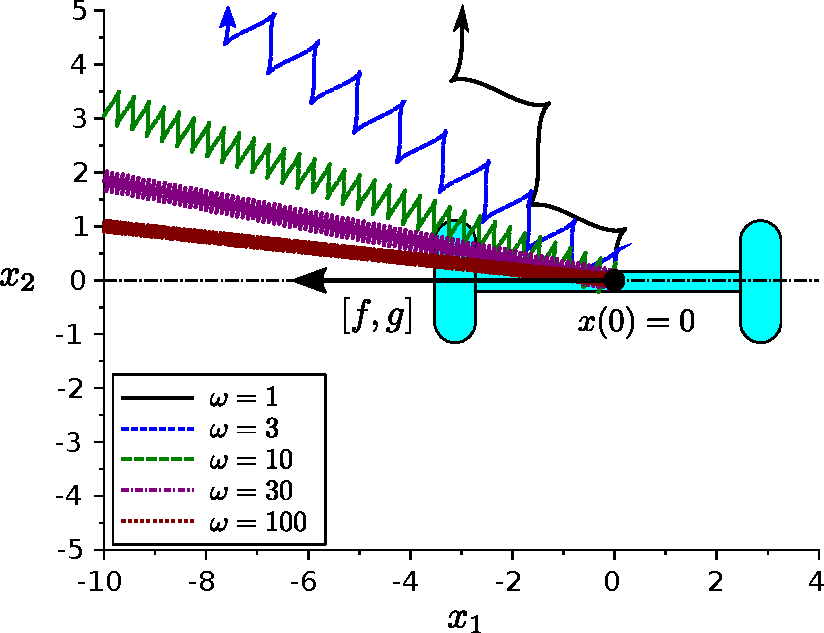
\includegraphics[width=0.75\textwidth]{roboter-averaging}
\par\end{centering}
\caption{Trajektorien des Robotermodells mit harmonischer Erregung~(\ref{eq:harmonisch-hochfreq-Erregung})
in der $(x_{1},x_{2})$-Ebene\label{fig:Trajektorien-Roboter-harmonische-Erregung}}
\end{figure}

Der Übergang von System~(\ref{eq:Umschaltsystem-zwei-VF}) mit den
Vektorfeldern~$f$ und~$g$ unter der Erregung~(\ref{eq:harmonisch-hochfreq-Erregung})
zu dem System~(\ref{eq:Lie-Klammer-harmonisch-Grenzsystem}) mit
der Lie-Klammer~$[f,g]$ lässt sich zur Steuerung bzw. Planung von
Bewegungsabläufen verwenden~\cite{sussmann1991cdc,lafferriere1993,kumar1999},
kommt aber auch in der Extremwertregelung zum Einsatz~\cite{duerr2013}.\nocite{nof1999}
Der Ansatz zur Bewegungsplanung soll für das System~(\ref{eq:Umschaltsystem-zwei-VF})
kurz erläutert werden. Durch passende Wahl der Eingänge~$u_{1}$
und~$u_{2}$ kann sich die Bahn des System~(\ref{eq:Umschaltsystem-zwei-VF})
in Richtung des Vektorfeldes~$f$ (mit $u_{1}=1,u_{2}=0$), des Vektorfeldes~$g$
(mit $u_{1}=0,u_{2}=1$) oder mit~(\ref{eq:harmonisch-hochfreq-Erregung})
in Richtung der Lie-Klammer $[f,g]$ bewegen. Prinzipiell sind auch
entsprechende Linearkombinationen der beteiligten Vektorfelder möglich.
Diese Betrachtung rechtfertigt den Übergang von dem gegebenen System~(\ref{eq:Umschaltsystem-zwei-VF})
zu dem erweiterten System (engl. \emph{Lie bracket extension})
\[
\dot{x}=v_{1}(t)f(x)+v_{2}(t)g(x)+v_{3}(t)[f,g](x)
\]
mit den neuen Eingängen $v_{1},v_{2},v_{3}$ (vgl.~\cite{sussmann1993}).
Die Bewegungsplanung auf Basis dieses Ansatzes wird beispielsweise
in~\cite{duleba1999} für das Model des mobilen Roboters erläutert.
Außerdem lässt sich dieses Mittelungsverfahren auch zur Extremalregelung
nutzen~\cite{duerr2013}.

\section{Distributionen und Kodistributionen\label{sec:Distributionen-und-Kodistributionen}}

Oft wird ein System durch mehrere gleichzeitig wirkende Vektorfelder
beschrieben, z.\,B. bei mehreren Eingängen, so dass sich das resultierende
Vektorfeld aus einer Linearkombination der beteiligten Vektorfelder
ergibt. In solchen Fällen bietet es sich an, von den einzelnen Vektorfeldern
zu dem von ihnen erzeugten geometrischem Objekt überzugehen. Dieser
Übergang führt auf das Konzept der Distribution. Die in diesem Abschnitt
enthaltene Einführung in Distributionen orientiert sich an~\cite[Abschnitt~{1.3}]{isidori3}.

Sei $\mathcal{M}\subseteq\R^{n}$ offen und $f_{1},\ldots,f_{k}:\mathcal{M}\to\R^{n}$
seien (hinreichend glatte) Vektorfelder. Diese Vektorfelder spannen
in jedem Punkt $x\in\mathcal{M}$ einen Untervektorraum des~$\R^{n}$
auf 
\begin{equation}
\spann\left\{ f_{1}(x),\ldots,f_{k}(x)\right\} ,\label{eq:VF-spannen-Dist-auf}
\end{equation}
wobei die beteiligten Vektorfelder nicht zwangsläufig linear unabhängig
sein müssen. Die Zuordnung eines Punktes $x\in\mathcal{M}$ zu einem
Untervektorraum des~$\R^{n}$ nennt man \emph{Distribution}\index{Distribution}:
\[
\mathcal{M}\ni x\mapsto\Delta(x)=\spann\left\{ f_{1}(x),\ldots,f_{k}(x)\right\} \subseteq\R^{n}.
\]
Ein Vektorfeld $f:\mathcal{M}\to\R^{n}$ liegt in der Distribution~$\Delta$,
wenn der Vektor $f(x)$ immer im Unterraum $\Delta(x)$ liegt, d.\,h.
$f\in\Delta$ bedeutet $f(x)\in\Delta(x)$ für alle $x\in\mathcal{M}$.

Wird die Distribution von glatten Vektorfeldern aufgespannt, so spricht
man von einer \emph{glatten Distribution}. Die Dimension einer Distribution~$\Delta$
im Punkt $x\in\mathcal{M}$ ist die Dimension des Unter\-vektor\-raumes
$\Delta(x)$. Eine Distribution~$\Delta$ heißt \emph{regulär}\index{Distribution!reguläre}
(im Punkt $p\in\mathcal{M}$), falls es eine Zahl $r\in\{0,\ldots,n\}$
gibt, so dass 
\[
\dim\,\Delta(x)=r
\]
 für alle~$x$ aus einer Umgebung von~$p$. Eine reguläre Distribution
hat also in der Umgebung des betreffenden Punktes eine konstante Dimension. 

Ist umgekehrt eine glatte Distribution~$\Delta$ gegeben, die im
Punkt $p\in\mathcal{M}$ regulär mit der Dimension~$r$ ist, dann
gibt es eine lokale Basisdarstellung der Distribution durch $r$ glatte
Vektorfelder~\cite[Lemma~{19.1}]{lee2006}. Genauer gesagt: Es gibt
eine Umgebung $\mathcal{U}\subseteq\mathcal{M}$ von~$p$ und $r$
glatte Vektorfelder $f_{1},\ldots,f_{r}:\mathcal{U}\to\R^{n}$ derart,
dass für alle $x\in\mathcal{U}$ gilt:
\begin{enumerate}
\item Die Vektoren $f_{1}(x),\ldots,f_{r}(x)$ sind linear unabhängig für
alle $x\in\mathcal{U}$,
\item $\Delta(x)=\spann\left\{ f_{1}(x),\ldots,f_{r}(x)\right\} $ auf~$\mathcal{U}$.
\end{enumerate}
Damit kann auf~$\mathcal{U}$ jedes Vektorfeld $f\in\Delta$ in der
Form
\begin{equation}
f(x)=\sum_{i=1}^{r}\alpha_{i}(x)f_{i}(x)\label{eq:Basisdarstellung-VF-Distr}
\end{equation}
dargestellt werden, wobei $\alpha_{1},\ldots,\alpha_{r}:\mathcal{U}\to\R$
glatte Skalarfelder sind. Gl.~(\ref{eq:Basisdarstellung-VF-Distr})
lässt sich als lineares Gleichungssystem 
\[
\left(f_{1}(x),\ldots,f_{r}(x)\right)\left(\begin{array}{c}
\alpha_{1}(x)\\
\vdots\\
\alpha_{r}(x)
\end{array}\right)=f(x)
\]
schreiben. Die Annahme $f\in\Delta$ besagt, dass das Vektorfeld~$f$
für alle $x\in\mathcal{U}$ in der linearen Hülle der Vektorfelder
$f_{1},\ldots,f_{r}$ liegt. Damit ist das lineare Gleichungssystem
lösbar.

Die Vektorfelder $f_{1},\ldots,f_{k}$ aus Gl.~(\ref{eq:VF-spannen-Dist-auf})
lassen sich spaltenweise zu einer $n\times k$-Matrix zusammenfassen:
\[
F(x)=\left(f_{1}(x),\ldots,f_{k}(x)\right).
\]
Dann gilt 
\[
\Delta(x)=\im\,F(x),
\]
so dass die Distribution von den Spalten von~$F$ aufgespannt wird.
Die Dimension der Distribution stimmt dann mit dem Rang der Matrix~$F$
überein: 
\[
\dim\,\Delta(x)=\rank\,F(x).
\]

\begin{example}
\label{exa:beispiel-distribution-rotation}Wir betrachten die von
den Vektorfeldern 
\[
f_{1}(x)=\sin x_{3}\frac{\partial}{\partial x_{1}}+\cos x_{3}\frac{\partial}{\partial x_{2}}\quad\mbox{und}\quad f_{2}(x)=-\cos x_{3}\frac{\partial}{\partial x_{1}}+\sin x_{3}\frac{\partial}{\partial x_{2}}
\]
im~$\R^{3}$ aufgespannte Distribution $\Delta=\spann\{f_{1},f_{2}\}$.
Die Vektorfelder~$f_{1}$ und~$f_{2}$ hängen von~$x_{3}$ ab,
die Distribution~$\Delta$ ist aber für ganz~$\R^{3}$ regulär mit
$\dim\,\Delta(x)=2$ und spannt für alle $x\in\R^{3}$ die $(x_{1},x_{2})$-Ebene
auf. Fasst man die Vektorfelder zu 
\[
F(x)=\left(f_{1}(x),f_{2}(x)\right)=\left(\begin{array}{cc}
\sin x_{3} & -\cos x_{3}\\
\cos x_{3} & \phantom{{-}}\sin x_{3}\\
0 & 0
\end{array}\right)
\]
zusammen, so beschreibt diese Matrix eine Rotation in der $(x_{1},x_{2}$)-Ebene
(vgl. Abb.~\ref{fig:beispiel-distribution-rotation}). Daher kann
die Beschreibung der Distribution (über die Auswahl einer Basis) zu
$\Delta=\spann\{\frac{\partial}{\partial x_{1}},\frac{\partial}{\partial x_{2}}\}$
vereinfacht werden. Die Distribution hängt damit nicht von~$x$ ab,
in jedem Punkt $x\in\mathcal{M}$ liefert $\Delta(x)$ den gleichen
Unterraum.
\end{example}
\begin{figure}
\begin{centering}
\resizebox{0.75\textwidth}{!}{\input{beispiel_distr_rotation.pdftex_t}}
\par\end{centering}
\caption{Vektorfelder $f_{1}$ und $f_{2}$ aus Beispiel~\ref{exa:beispiel-distribution-rotation}
für $p=0$ und $q=(0,0,\pi/4)^{T}$\label{fig:beispiel-distribution-rotation}}

\end{figure}

Im Bildbereich ist der Wert $\Delta(x)$ einer Distribution ein Unter\-vektor\-raum,
d.\,h. $\Delta(x)\subseteq\R^{n}$. \emph{Summe} und \emph{Durchschnitt}
von Unter\-vektor\-räumen lassen sich daher punktweise auf Distributionen
übertragen: 
\[
\begin{array}{rclcl}
\left(\Delta_{1}+\Delta_{2}\right)(x) & := & \Delta_{1}(x) & + & \Delta_{2}(x),\\
\left(\Delta_{1}\cap\Delta_{2}\right)(x) & := & \Delta_{1}(x) & \cap & \Delta_{2}(x).
\end{array}
\]
Für glatte Distributionen in der Umgebung eines regulären Punktes
sind auch Durchschnitt und Summe glatte Distributionen. Über die betreffenden
Untervektorräume im Bildbereich lassen sich auch die üblichen Teilmengen-
bzw. Unterraumrelationen für Distributionen definieren, z.\,B. 
\[
\begin{array}{rccl}
\Delta_{1}\subseteq\Delta_{2} & :\Longleftrightarrow & \forall x\in\mathcal{M}: & \Delta_{1}(x)\subseteq\Delta_{2}(x),\\
\Delta_{1}\subset\Delta_{2} & :\Longleftrightarrow & \forall x\in\mathcal{M}: & \Delta_{1}(x)\subset\Delta_{2}(x).
\end{array}
\]

Seien $\omega_{1},\ldots,\omega_{k}:\mathcal{M}\to(\R^{n})^{*}$ Kovektorfelder.
Diese spannen im Dualraum~$(\R^{n})^{*}$ des~$\R^{n}$ eine \emph{Kodistribution}\index{Kodistribution}
auf: 
\[
\Omega=\spann\left\{ \omega_{1},\ldots,\omega_{k}\right\} .
\]
 Dabei wird jedem Punkt~$x$ mit
\[
\mathcal{M}\ni x\mapsto\Omega(x)=\spann\left\{ \omega_{1}(x),\ldots,\omega_{k}(x)\right\} \subseteq(\R^{n})^{*}
\]
ein Untervektorraum des Dualraums zugeordnet. Bei Kodistributionen
sind Dimension, Summe, Durchschnitt usw. analog zu Distributionen
definiert.

\medskip{}

Für eine gegebene Distribution $\Delta$ ist der \emph{Annihilator}\index{Annihilator}
(auch \emph{Annulator}\index{Annulator} genannt)~$\Delta^{\perp}$
durch 
\[
\Delta^{\perp}(x)=\left\{ \omega\in(\R^{n})^{*};\,\left\langle \omega,f\right\rangle =0\mbox{ für alle }f\in\Delta(x)\right\} 
\]
definiert, d.\,h.~$\Delta^{\perp}$ ist eine Kodistribution. Der
Annihilator~$\Omega^{\perp}$\index{Annihilator} einer Kodistribution~$\Omega$
ist die durch 
\[
\Omega^{\perp}(x)=\left\{ f\in\R^{n};\,\left\langle \omega,f\right\rangle =0\mbox{ für alle }\omega\in\Omega(x)\right\} 
\]
definierte Distribution. Mit dem Annihilator wird der von der jeweiligen
Distribution bzw. Kodistribution erzeugte Untervektorraum um sein
orthogonales Komplement im Sinne der natürlichen Paarung ergänzt (vgl.
Abschnitt~\ref{sec:Lineare-Algebra}).

\begin{example}
\label{exa:Annihilator1}Man betrachte die von den Vektorfeldern 
\[
f_{1}(x)=\sin x_{3}\frac{\partial}{\partial x_{1}}+\cos x_{3}\frac{\partial}{\partial x_{2}}\quad\mbox{und}\quad f_{2}(x)=\frac{\partial}{\partial x_{3}}
\]
des mobilen Roboters aufgespannte Distribution $\Delta=\spann\{f_{1},f_{2}\}$.
In \textsc{Maxima} steht für die Berechnung des orthogonalen Komplements\index{orthogonales Komplement}
die Routine \hbox{\texttt{orthogonal\_complement}} zur Verfügung,
wobei die betreffenden Vektoren bzw. Vektorfelder als Spaltenvektoren
zu übergeben sind (vgl. Beispiel~\ref{exa:orthogonales-Komplement}).
Dabei liest man den Annihilator\index{Annihilator} 
\[
\Delta^{\perp}(x)=\spann\{-\cos x_{3}\,\d x_{1}+\sin x_{3}\,\d x_{2}\}
\]
ab, der zwar von Maxima als Spaltenvektor geliefert wird, hier aber
als Zeilenvektor bzw. Kovektorfeld zu verstehen ist. Die vom Programm
getroffene Zusatzannahme $\sin x_{3}\neq0$ ist der internen Implementierung
in \textsc{Maxima} geschuldet und hier nicht weiter von Bedeutung.

\begin{maxima}\noindent
%%%%%%%%%%%%%%%
%%% INPUT:
\begin{minipage}[t]{8ex}
\color{red}\bf
\begin{verbatim}
(%i1) 
\end{verbatim}
\end{minipage}
\begin{minipage}[t]{\textwidth}
\color{blue}
\begin{verbatim}
load("eigen")$
\end{verbatim}
\end{minipage}


\noindent
%%%%%%%%%%%%%%%
%%% INPUT:
\begin{minipage}[t]{8ex}
\color{red}\bf
\begin{verbatim}
(%i2) 
\end{verbatim}
\end{minipage}
\begin{minipage}[t]{\textwidth}
\color{blue}
\begin{verbatim}
f1:columnvector([sin(x3),cos(x3),0]);
\end{verbatim}
\end{minipage}
%%% OUTPUT:
\begin{math}\displaystyle
\parbox{8ex}{\color{labelcolor}(\%o2) }
\begin{pmatrix}\mathrm{sin}\left( x3\right) \cr \mathrm{cos}\left( x3\right) \cr 0\end{pmatrix}
\end{math}
%%%%%%%%%%%%%%%


\noindent
%%%%%%%%%%%%%%%
%%% INPUT:
\begin{minipage}[t]{8ex}
\color{red}\bf
\begin{verbatim}
(%i3) 
\end{verbatim}
\end{minipage}
\begin{minipage}[t]{\textwidth}
\color{blue}
\begin{verbatim}
f2:columnvector([0,0,1]);
\end{verbatim}
\end{minipage}
%%% OUTPUT:
\begin{math}\displaystyle
\parbox{8ex}{\color{labelcolor}(\%o3) }
\begin{pmatrix}0\cr 0\cr 1\end{pmatrix}
\end{math}
%%%%%%%%%%%%%%%


\noindent
%%%%%%%%%%%%%%%
%%% INPUT:
\begin{minipage}[t]{8ex}
\color{red}\bf
\begin{verbatim}
(%i4) 
\end{verbatim}
\end{minipage}
\begin{minipage}[t]{\textwidth}
\color{blue}
\begin{verbatim}
Ann:orthogonal_complement(f1,f2);
\end{verbatim}
\end{minipage}
%%% OUTPUT:
\begin{math}\displaystyle
Proviso: \mathrm{notequal}\left( \mathrm{sin}\left( x3\right) ,0\right)  \;\wedge\; \mathrm{notequal}\left( \mathrm{sin}\left( x3\right) ,0\right) 
\end{math}

\noindent
\begin{math}\displaystyle
\parbox{8ex}{\color{labelcolor}(\%o4) }
\mathrm{span}\left( \begin{pmatrix}−\mathrm{cos}\left( x3\right) \cr \mathrm{sin}\left( x3\right) \cr 0\end{pmatrix}\right) 
\end{math}
%%%%%%%%%%%%%%%

\end{maxima}
\end{example}

Den Annihilator kann man direkt über Matrizen darstellen bzw. berechnen.
Dazu fasst man die Vektorfelder $f_{1},\ldots,f_{k}:\mathcal{M}\to\R^{n}$,
welche die Distribution~$\Delta$ aufspannen, bzw. jene Kovektorfelder
$\omega_{1},\ldots,\omega_{k}:\mathcal{M}\to(\R^{n})^{*}$, die die
Kodistribution~$\Omega$ bilden, zusammen: 
\[
F(x)=\left(f_{1}(x),\ldots,f_{k}(x)\right)\quad\mbox{und}\quad W(x)=\left(\begin{array}{c}
\omega_{1}(x)\\
\vdots\\
\omega_{k}(x)
\end{array}\right).
\]
Der Annihilator~$\Delta^{\perp}$ wird von denjenigen Kovektoren~$\omega$
aufgespannt, welche die Bedingung $\omega\,F(x)=0$ erfüllen. Ähnlich
wird der Annihilator~$\Omega^{\perp}$ von Vektoren~$f$ mit $W(x)\,f=0$
aufgespannt. Das ist der Kern der Matrix~$W$, d.\,h. 
\begin{equation}
\Omega^{\perp}(x)=\ker\,W(x).\label{eq:Ann-Kern-W}
\end{equation}
Den Annihilator der Distribution~$\Delta$ erhält man mittels 
\begin{equation}
\Delta^{\perp}(x)\cong\ker\,F^{T}(x).\label{eq:Ann-Kern-FT}
\end{equation}
Da der Kern einer Matrix in Abschnitt~\ref{sec:Lineare-Algebra}
als lineare Hülle von Spaltenvektoren eingeführt wurde, der Annihilator
einer Distribution aber von Kovektorfeldern aufgespannt wird, wären
die auf der rechten Seite von~(\ref{eq:Ann-Kern-FT}) berechneten
Basisvektorfelder durch Transposition noch in den Dualraum zu übertragen.
Dabei nutzt man die Isomorphie zwischen dem Primalraum~$\R^{n}$
und seinem Dualraum~$(\R^{n})^{*}$ aus. In~(\ref{eq:Ann-Kern-FT})
wird diese Beziehung durch das Symbol ,,$\cong$`` anstelle des
Gleichheitszeichens ausgedrückt.

\begin{example}
\label{exa:Annihilator2}Wir betrachten die von den Vektorfeldern
$f_{1},f_{2}$ aufgespannte Distribution~$\Delta$ aus Beispiel~\ref{exa:Annihilator1}.
Entsprechend Gl.~(\ref{eq:Ann-Kern-FT}) lässt sich der Annihilator\index{Annihilator}
über den Kern der Matrix
\[
F^{T}(x)=\left(\begin{array}{c}
f_{1}^{T}(x)\\
f_{2}^{T}(x)
\end{array}\right)=\left(\begin{array}{ccc}
\sin x_{3} & \cos x_{3} & 0\\
0 & 0 & 1
\end{array}\right)
\]
berechnen. Die Vektorfelder werden als Listen angelegt und zeilenweise
zur Matrix~$F^{T}$ zusammengefügt. Der berechnete Annihilator stimmt
mit dem Ergebnis aus Beispiel~\ref{exa:Annihilator1} überein:

\begin{maxima}\noindent
%%%%%%%%%%%%%%%
%%% INPUT:
\begin{minipage}[t]{8ex}
\color{red}\bf
\begin{verbatim}
(%i1) 
\end{verbatim}
\end{minipage}
\begin{minipage}[t]{\textwidth}
\color{blue}
\begin{verbatim}
f1:[sin(x3),cos(x3),0];
f2:[0,0,1];
\end{verbatim}
\end{minipage}
%%% OUTPUT:
\begin{math}\displaystyle
\parbox{8ex}{\color{labelcolor}(\%o1) }
[\mathrm{sin}\left( x3\right) ,\mathrm{cos}\left( x3\right) ,0]
\end{math}

\begin{math}\displaystyle
\parbox{8ex}{\color{labelcolor}(\%o2) }
[0,0,1]
\end{math}
%%%%%%%%%%%%%%%


\noindent
%%%%%%%%%%%%%%%
%%% INPUT:
\begin{minipage}[t]{8ex}
\color{red}\bf
\begin{verbatim}
(%i3) 
\end{verbatim}
\end{minipage}
\begin{minipage}[t]{\textwidth}
\color{blue}
\begin{verbatim}
FT:matrix(f1,f2);
\end{verbatim}
\end{minipage}
%%% OUTPUT:
\begin{math}\displaystyle
\parbox{8ex}{\color{labelcolor}(\%o3) }
\begin{pmatrix}\mathrm{sin}\left( x3\right)  & \mathrm{cos}\left( x3\right)  & 0\cr 0 & 0 & 1\end{pmatrix}
\end{math}
%%%%%%%%%%%%%%%


\noindent
%%%%%%%%%%%%%%%
%%% INPUT:
\begin{minipage}[t]{8ex}
\color{red}\bf
\begin{verbatim}
(%i4) 
\end{verbatim}
\end{minipage}
\begin{minipage}[t]{\textwidth}
\color{blue}
\begin{verbatim}
Ann:nullspace(FT);
\end{verbatim}
\end{minipage}
%%% OUTPUT:
\begin{math}\displaystyle
Proviso: \mathrm{notequal}\left( \mathrm{sin}\left( x3\right) ,0\right) \;\wedge\; \mathrm{notequal}\left( \mathrm{sin}\left( x3\right) ,0\right) 
\end{math}

\noindent
\begin{math}\displaystyle
\parbox{8ex}{\color{labelcolor}(\%o4) }
\mathrm{span}\left( \begin{pmatrix}−\mathrm{cos}\left( x3\right) \cr \mathrm{sin}\left( x3\right) \cr 0\end{pmatrix}\right) 
\end{math}
%%%%%%%%%%%%%%%
\end{maxima}
\end{example}

\begin{example}
\label{exa:Annihilator3}Bei der in den Beispielen~\ref{exa:Annihilator1}
und~\ref{exa:Annihilator2} betrachteten Berechnung des Annihilators
liegt eine sehr spezielle Situation vor, nämlich eine von zwei (linear
unabhängigen) Vektorfeldern aufgespannte Distribution im Vektorraum~$\R^{3}$.
In diesem Sonderfall lässt sich über das Kreuzprodukt 
\[
f_{1}(x)\times f_{2}(x)=\left(\begin{array}{c}
\phantom{{-}}\cos x_{3}\\
-\sin x_{3}\\
0
\end{array}\right)
\]
eine Basis für den Annihilator angeben. Das Kreuzprodukt\index{Kreuzprodukt}\index{Produkt!Kreuz-}
steht senkrecht auf der von $f_{1}(x)$ und $f_{2}(x)$ aufgespannten
Ebene: 
\begin{eqnarray*}
\Delta^{\perp}(x) & = & \spann\left\{ \left(f_{1}(x)\times f_{2}(x)\right)^{T}\right\} \\
 & = & \spann\left\{ \left(\cos x_{3},-\sin x_{3},0\right)\right\} .
\end{eqnarray*}
Das gegenüber den Beispielen~\ref{exa:Annihilator1} und~\ref{exa:Annihilator2}
abweichende Vorzeichen des den Annihilator aufspannenden Kovektorfeldes
ändert nichts am Annihilator selbst. Zur Berechnung des Kreuzprodukts
steht in dem \textsc{Maxima}-Paket \texttt{vect} die binäre Operation
,,$\sim$`` zur Verfügung, die mit der Funktion \texttt{express}
ausgewertet wird:
\end{example}
\begin{maxima}\noindent
%%%%%%%%%%%%%%%
%%% INPUT:
\begin{minipage}[t]{8ex}
\color{red}\bf
\begin{verbatim}
(%i1) 
\end{verbatim}
\end{minipage}
\begin{minipage}[t]{\textwidth}
\color{blue}
\begin{verbatim}
load("vect")$
\end{verbatim}
\end{minipage}

\smallskip

\noindent
%%%%%%%%%%%%%%%
%%% INPUT:
\begin{minipage}[t]{8ex}
\color{red}\bf
\begin{verbatim}
(%i2) 
\end{verbatim}
\end{minipage}
\begin{minipage}[t]{\textwidth}
\color{blue}
\begin{verbatim}
f1:[sin(x3),cos(x3),0];
f2:[0,0,1];
\end{verbatim}
\end{minipage}
%%% OUTPUT:
\begin{math}\displaystyle
\parbox{8ex}{\color{labelcolor}(\%o2) }
[\mathrm{sin}\left( x3\right) ,\mathrm{cos}\left( x3\right) ,0]
\end{math}

\noindent
\begin{math}\displaystyle
\parbox{8ex}{\color{labelcolor}(\%o3) }
[0,0,1]
\end{math}
%%%%%%%%%%%%%%%


\noindent
%%%%%%%%%%%%%%%
%%% INPUT:
\begin{minipage}[t]{8ex}
\color{red}\bf
\begin{verbatim}
(%i4) 
\end{verbatim}
\end{minipage}
\begin{minipage}[t]{\textwidth}
\color{blue}
\begin{verbatim}
express(f1~f2);
\end{verbatim}
\end{minipage}
%%% OUTPUT:
\begin{math}\displaystyle
\parbox{8ex}{\color{labelcolor}(\%o4) }
[\mathrm{cos}\left( x3\right) ,-\mathrm{sin}\left( x3\right) ,0]
\end{math}
%%%%%%%%%%%%%%%
\end{maxima}

\begin{example}
\label{exa:Annihilator-Kodistribution}Man betrachtet das auf der
Menge $\mathcal{M}=\R^{3}\setminus\{0\}$ definierte Skalarfeld $h(x)=x_{1}^{2}+x_{2}^{2}$
, welches bereits in den Beispielen~\ref{exa:Lie-Skalar1} und~\ref{exa:Lie-Kovektor}
Verwendung fand. Der Gradient $\d h(x)=(2x_{1},2x_{2},0)$ ist ein
Kovektorfeld, welches die eindimensionale Kodistribution $\Omega:=\spann\{\d h\}$
aufspannt. Der Annihilator $\Omega^{\perp}$ ist eine zweidimensionale
Distribution 
\[
\Omega^{\perp}=\spann\left\{ -2x_{2}\frac{\partial}{\partial x_{3}},-2x_{2}\frac{\partial}{\partial x_{1}}+2x_{1}\frac{\partial}{\partial x_{2}}\right\} ,
\]
die man auf Basis von Gl.~(\ref{eq:Ann-Kern-W}) mit \textsc{Maxima}
berechnen kann:

\begin{maxima}\noindent
%%%%%%%%%%%%%%%
%%% INPUT:
\begin{minipage}[t]{8ex}
\color{red}\bf
\begin{verbatim}
(%i1) 
\end{verbatim}
\end{minipage}
\begin{minipage}[t]{\textwidth}
\color{blue}
\begin{verbatim}
h:x1^2+x2^2$
dh:jacobian([h],[x1,x2,x3]);
\end{verbatim}
\end{minipage}
%%% OUTPUT:
\begin{math}\displaystyle
\parbox{8ex}{\color{labelcolor}(\%o2) }
\begin{pmatrix}2\,x1 & 2\,x2 & 0\end{pmatrix}
\end{math}
%%%%%%%%%%%%%%%


\noindent
%%%%%%%%%%%%%%%
%%% INPUT:
\begin{minipage}[t]{8ex}
\color{red}\bf
\begin{verbatim}
(%i3) 
\end{verbatim}
\end{minipage}
\begin{minipage}[t]{\textwidth}
\color{blue}
\begin{verbatim}
D:nullspace(dh);
\end{verbatim}
\end{minipage}
%%% OUTPUT:
\begin{math}\displaystyle
Proviso: \mathrm{notequal}\left( 2\,x1,0\right) 
\end{math}

\noindent
\begin{math}\displaystyle
\parbox{8ex}{\color{labelcolor}(\%o3) }
\mathrm{span}\left( \begin{pmatrix}0\cr 0\cr -2\,x2\end{pmatrix},\begin{pmatrix}-2\,x2\cr 2\,x1\cr 0\end{pmatrix}\right) 
\end{math}
%%%%%%%%%%%%%%%
\end{maxima}
\end{example}
\medskip{}

Im Bildbereich sind Distributionen Untervektorräume. Dadurch lassen
sich gängige Eigenschaften von Unterräumen unmittelbar auf Distributionen
übertragen.
\begin{proposition}
\label{pro:Annihilator}Seien $\Delta$, $\Delta_{1}$ und $\Delta_{2}$
auf $\mathcal{M}\subseteq\R^{n}$ definierte Distributionen. Zwischen
den Distributionen und ihren Annihilatoren gelten folgende Beziehungen:
\begin{subequations}
\begin{gather}
\dim(\Delta)+\dim(\Delta^{\perp})=n\label{eq:dimensionssatz-distr-annihilator}\\
\Delta_{1}\subseteq\Delta_{2}\quad\Longleftrightarrow\quad\Delta_{1}^{\perp}\supseteq\Delta_{2}^{\perp}\label{eq:Annihilator-Subseteq}\\
\Delta_{1}\subset\Delta_{2}\quad\Longleftrightarrow\quad\Delta_{1}^{\perp}\supset\Delta_{2}^{\perp}\label{eq:eq:Annihilator-Subset}\\
\left(\Delta_{1}\cap\Delta_{2}\right)^{\perp}=\Delta_{1}^{\perp}+\Delta_{2}^{\perp}\label{eq:Annihilator-Schnitt}\\
\left(\Delta_{1}+\Delta_{2}\right)^{\perp}=\Delta_{1}^{\perp}\cap\Delta_{2}^{\perp}\label{eq:Annihilator-Summe}
\end{gather}
\end{subequations}
\end{proposition}
Gl.~(\ref{eq:dimensionssatz-distr-annihilator}) ist eine unmittelbare
Folgerung aus der Dimensions\-formel\index{Dimensionsformel}~(\ref{eq:dimensionsformel-ortho-kompl}).
Gln.~(\ref{eq:Annihilator-Subseteq}) bis~(\ref{eq:Annihilator-Summe})
ergeben sich aus den entsprechenden Aussagen für Unter\-vektor\-räume
(siehe Übungsaufgabe~\ref{aufgabe-diff-Annihilator}). \medskip{}

Bei einer glatten Distribution ist es nicht ausgeschlossen, dass es
einen lokalen Abfall der Dimension gibt, d.\,h. die Dimension in
einigen Punkten kleiner ist als in deren Umgebung. An den betreffenden
Punkten des Definitionsbereichs~$\mathcal{M}$ müsste sich nach Gl.~(\ref{eq:dimensionssatz-distr-annihilator})
die Dimension des Annihilators entsprechend erhöhen. In solchen Fällen
wäre der Annihilator nicht mehr glatt. Umgekehrt kann eine nicht glatte
Distribution durchaus einen glatten Annihilator besitzen. Derartige
pathologische Fälle sind allerdings in der Nähe eines regulären Punktes
ausgeschlossen~\cite[Lemma~{1.3.6}]{isidori3}:
\begin{lemma}
\label{lem:Annihilator-in-regulaerem-Punkt}Sei $\Delta$ eine glatte
Distribution, die im Punkt $p\in\mathcal{M}$ regulär ist. Dann ist
der Annihilator~$\Delta^{\perp}$ebenfalls im Punkt~$p$ regulär.
Außerdem gibt es eine offene Umgebung $\mathcal{U}\subseteq\mathcal{M}$
von~$p$, so dass $\Delta^{\perp}$ auf~$\mathcal{U}$ eine glatte
Kodistribution ist.
\end{lemma}

\section{Involutive Distributionen\label{sec:Involutive-Distributionen}}

Jedes glatte Vektorfeld besitzt einen eindeutigen lokalen Fluss. Fasst
man dagegen mehrere Vektorfelder in einer Distribution zusammen, so
kann die Verknüpfung der Flüsse dieser Vektorfelder möglicherweise
in eine (neue) Richtung zeigen, die nicht von den beteiligten Vektorfeldern
selber, sondern von deren Lie-Klammern aufgespannt wird (vgl. Abschnitt~\ref{sec:Lie-Klammern-dynamische-Systeme}).
Dieser Abschnitt befasst sich mit den damit verbundenen Fragestellungen,
z.\,B. unter welchen Bedingungen eine Distribution schon alle möglichen
Richtungen erfasst oder welche Konsequenzen diese Eigenschaft für
den Annihilator hat.

\medskip{}

Alle in diesem Abschnitt betrachteten Felder und Distributionen seien
auf einer offenen Teilmenge $\mathcal{M}\subseteq\R^{n}$ definiert
und hinreichend glatt. Sei $f:\mathcal{M}\to\R^{n}$ ein Vektorfeld.
Eine Distribution $\Delta$ heißt \emph{invariant}\index{Distribution!invariante}
unter dem Vektorfeld~$f$ (kurz \emph{$f$-invariant}), wenn gilt
\begin{equation}
\forall g\in\Delta:\quad[f,g]\in\Delta.\label{eq:invariant}
\end{equation}
Eine Distribution ist involutiv, wenn sie für jedes ihrer Vektorfelder
invariant ist. Genauer: Eine Distribution $\Delta$ heißt \emph{involutiv}\index{Distribution!involutive}\index{involutive Distribution},
wenn gilt 
\begin{equation}
\forall f,g\in\Delta:\quad[f,g]\in\Delta.\label{eq:involutiv}
\end{equation}
Da bei einer involutiven Distribution nach Gl.~(\ref{eq:involutiv})
auch alle Lie-Klammern der beteiligten Vektorfelder in der Distribution
liegen, ist eine involutive Distribution zugleich eine Lie-Algebra\index{Lie-Algebra}\index{Algebra!Lie-}
(vgl. Anmerkung~\ref{rem:Lie-Algebra}).

Im Abschnitt~\ref{sec:Lie-Klammern-dynamische-Systeme} wurde gezeigt,
dass die Verkettung der Flüsse zweier Vektor\-felder auch eine neue
Trajektorie generieren kann. Diese zusätzliche Bewegungsrichtung lässt
sich als Fluss der Lie-Klammern der beteiligten Vektor\-felder darstellen.
Schließt umgekehrt die betreffende Distribution entsprechend Gl.~(\ref{eq:involutiv})
die Lie-Klammern aller beteiligten Vektorfelder mit ein, so kann jede
durch Fluss\-verkettung dieser Vektorfelder erzeugte Lösungsrichtung
auch direkt von einem Vektorfeld der Distribution erzeugt werden.

Gl.~(\ref{eq:involutiv}) wäre (außer im Fall einer Distribution
der Dimension Null) für unendlich viele Vektorfelder zu prüfen, nämlich
für alle Linearkombinationen der Basisvektorfelder. Glücklicherweise
reicht es aus, die Eigenschaft~(\ref{eq:involutiv}) nur für jene
Vektorfelder, welche die Distribution aufspannen, zu verifizieren:
\begin{lemma}
\label{lem:Involutivitaetstest-mit-basis}Sei $\Delta=\spann\left\{ f_{1},\ldots,f_{r}\right\} $
mit glatten Vektorfeldern $f_{1},\ldots,f_{r}:\mathcal{M}\to\R^{n}$.
Die Distribution~$\Delta$ ist genau dann involutiv, wenn 
\begin{equation}
[f_{i},f_{j}]\in\Delta\quad\mbox{für}\quad1\leq i,j\leq r.\label{eq:involutiv-Basisvektorfelder}
\end{equation}
\end{lemma}
\begin{svmultproof2}
\notwendig\ Wenn~(\ref{eq:involutiv}) für alle Vektorfelder der
Distribution gilt, dann muss es auch für die Basisvektorfelder $f_{1},\ldots,f_{r}$
gelten, d.\,h. Bedingung~(\ref{eq:involutiv-Basisvektorfelder})
ist erfüllt.

\hinreichend\ Wegen $f,g\in\Delta$ gibt es Skalarfelder $\alpha_{1},\ldots,\alpha_{r}$
und $\beta_{1},\ldots,\beta_{r}$ mit 
\begin{eqnarray*}
f(x) & = & \sum_{i=1}^{r}\alpha_{i}(x)f_{i}(x)\\
g(x) & = & \sum_{i=1}^{r}\beta_{i}(x)f_{i}(x).
\end{eqnarray*}
Gl.~(\ref{eq:Rechenregel-LK2}) liefert 
\[
\begin{array}{rcl}
[f,g] & = & [\sum\limits _{i=1}^{r}\alpha_{i}f_{i},\sum\limits _{i=1}^{r}\beta_{i}f_{i}]\\
 & = & \sum\limits _{i=1}^{r}\sum\limits _{j=1}^{r}\left(\alpha_{i}\beta_{j}[f_{i},f_{j}]+\alpha_{i}(L_{f_{i}}\beta_{j})f_{j}-\beta_{j}(L_{f_{j}}\alpha_{i})f_{i}\right),
\end{array}
\]
d.\,h. 
\[
[f,g]\in\underbrace{\spann\left\{ f_{1},\ldots,f_{r}\right\} }_{{\displaystyle =\Delta}}+\underbrace{\spann\left\{ [f_{i},f_{j}],\;1\leq i,j\leq r\right\} }_{{\displaystyle \subseteq\Delta\mbox{ wegen }(\ref{eq:involutiv-Basisvektorfelder})}}=\Delta,
\]
also gilt~(\ref{eq:involutiv}).
\end{svmultproof2}

Die Involutivitätsbedingung aus Lemma~\ref{lem:Involutivitaetstest-mit-basis}
lässt sich leicht implementieren (siehe Alg.~\ref{alg:Test-Involutivitaet}).
Der \textsc{Maxima}-Funktion \texttt{Involutivep} wird die zu prüfende
Distribution als eine Liste von Vektorfeldern $f_{1},\ldots,f_{r}$
übergeben und in eine Matrix umgewandelt. Bei Hinzunahme von Lie-Klammern
$[f_{i},f_{j}]$ darf sich im Falle einer involutiven Distribution
der Rang nicht erhöhen. Aufgrund der Schiefsymmetrie der Lie-Klammer
(siehe Prop.~\ref{prop:Eigenschaften-Lie-Klammer}) genügt es, die
Lie-Klammern $[f_{i},f_{j}]$ für $i=1,\ldots,r$ und $j=i+1,\ldots,r$
zu prüfen.

\begin{algorithm}
\noindent
%%%%%%%%%%%%%%%
%%% INPUT:
%\begin{minipage}[t]{8ex}
%\color{red}\bf
%\begin{verbatim}
%(%i11) 
%\end{verbatim}
%\end{minipage}
\begin{minipage}[t]{\textwidth}
\color{blue}
\begin{verbatim}
Involutivep(L,x):=block([F,G,i,j,r],
    r:length(L),
    F:apply('matrix,L),
    F:transpose(F),
    G:copy(F),  
    for i:1 thru r do 
        for j:i+1 thru r do block([f1,f2],
            f1:list_matrix_entries(col(F,i)),
            f2:list_matrix_entries(col(F,j)),
            G:addcol(G,LieBracket(f1,f2,x))
    ),
    is(rank(F)=rank(G))
)$
\end{verbatim}
\end{minipage}


\caption{Test eines Distribution auf Involutivität\label{alg:Test-Involutivitaet}}

\end{algorithm}

\begin{example}
\label{exa:Roboter-Test-Involutivitaet}Die von den Vektorfeldern
\[
f_{1}(x)=\sin x_{3}\frac{\partial}{\partial x_{1}}+\cos x_{3}\frac{\partial}{\partial x_{2}}\quad\mbox{und}\quad f_{2}(x)=\frac{\partial}{\partial x_{3}}
\]
des mobilen Roboters aufgespannte Distribution $\Delta=\spann\{f_{1},f_{2}\}$
ist auf Involutitvität zu untersuchen. Die Lie-Klammer der die Distribution
aufspannenden Vektorfelder~$f_{1}$ und~$f_{2}$ wurde bereits in
Beispiel~\ref{exa:Lie-Vektorfeld-Roboter} berechnet:
\[
[f_{1},f_{2}]=-\cos x_{3}\frac{\partial}{\partial x_{1}}+\sin x_{3}\frac{\partial}{\partial x_{2}}
\]
Wir fassen die drei Vektorfelder zu einer Matrix zusammen: 
\[
F(x)=\left(f_{1}(x),f_{2}(x),[f_{1},f_{2}](x)\right)=\left(\begin{array}{ccc}
\sin x_{3} & 0 & -\cos x_{3}\\
\cos x_{3} & 0 & \phantom{{-}}\sin x_{3}\\
0 & 1 & 0
\end{array}\right).
\]
Wegen $\det F(x)\equiv-1$ sind die beteiligten Vektorfelder linear
unabhängig. Daher lässt sich die Lie-Klammer $[f_{1},f_{2}]$ nicht
als Linearkombination der Vektorfelder $f_{1},f_{2}$ darstellen,
also gilt $[f_{1},f_{2}]\notin\Delta$. Die Distribution~$\Delta$
ist daher nicht involutiv.

Für die Überprüfung mit \textsc{Maxima} definiert man die Vektorfelder~$f_{1},f_{2}$
sowie~$x$ als Listen. Die Distribution $\Delta=\spann\{f_{1},f_{2}\}$,
die als Liste der Vektorfelder~$f_{1}$ und~$f_{2}$ an die in Alg.~\ref{alg:Test-Involutivitaet}
definierte \textsc{Maxima}-Funktion \texttt{Involtuivep} übergeben
wird, ist (wie bereits festegestellt wurde) nicht involutiv. Ergänzt
man die Distribution~$\Delta$ um die Lie-Klammer $[f_{1},f_{2}]$,
so erhält man eine involutive Distribution:

\begin{maxima}\noindent
%%%%%%%%%%%%%%%
%%% INPUT:
\begin{minipage}[t]{8ex}
\color{red}\bf
\begin{verbatim}
(%i5) 
\end{verbatim}
\end{minipage}
\begin{minipage}[t]{\textwidth}\color{blue}
\begin{verbatim}
f1:[sin(x3),cos(x3),0];
f2:[0,0,1];
x:[x1,x2,x3];
\end{verbatim}
\end{minipage}
%%% OUTPUT:
\begin{math}\displaystyle
\parbox{8ex}{\color{labelcolor}(\%o3) }
[\mathrm{sin}\left( x3\right) ,\mathrm{cos}\left( x3\right) ,0]
\end{math}

\noindent
\begin{math}\displaystyle
\parbox{8ex}{\color{labelcolor}(\%o4) }
[0,0,1]
\end{math}

\noindent
\begin{math}\displaystyle
\parbox{8ex}{\color{labelcolor}(\%o5) }
[x1,x2,x3]
\end{math}
%%%%%%%%%%%%%%%

\noindent
%%%%%%%%%%%%%%%
%%% INPUT:
\begin{minipage}[t]{8ex}
\color{red}\bf
\begin{verbatim}
(%i7) 
\end{verbatim}
\end{minipage}
\begin{minipage}[t]{\textwidth}
\color{blue}
\begin{verbatim}
D:[f1,f2];
Involutivep(D,x);
\end{verbatim}
\end{minipage}

%%% OUTPUT:
\noindent
\begin{math}\displaystyle
\parbox{8ex}{\color{labelcolor}(\%o6) }
[[\mathrm{sin}\left( x3\right) ,\mathrm{cos}\left( x3\right) ,0],[0,0,1]]
\end{math}

\noindent
\begin{math}\displaystyle
\parbox{8ex}{\color{labelcolor}(\%o7) }
false
\end{math}
%%%%%%%%%%%%%%%


\noindent
%%%%%%%%%%%%%%%
%%% INPUT:
\begin{minipage}[t]{8ex}
\color{red}\bf
\begin{verbatim}
(%i9) 
\end{verbatim}
\end{minipage}
\begin{minipage}[t]{\textwidth}
\color{blue}
\begin{verbatim}
I:endcons(LieBracket(f1,f2,x),D);
Involutivep(I,x);
\end{verbatim}
\end{minipage}

%%% OUTPUT:
\noindent
\begin{math}\displaystyle
\parbox{8ex}{\color{labelcolor}(\%o8) }
[[\mathrm{sin}\left( x3\right) ,\mathrm{cos}\left( x3\right) ,0],[0,0,1],[-\mathrm{cos}\left( x3\right) ,\mathrm{sin}\left( x3\right) ,0]]
\end{math}

\noindent
\begin{math}\displaystyle
\parbox{8ex}{\color{labelcolor}(\%o9) }
true
\end{math}
%%%%%%%%%%%%%%%
\end{maxima}
\end{example}

Involutive Distributionen können immer von kommutierenden Vektorfeldern
aufgespannt werden:
\begin{lemma}
\label{lem:Basisdarstellung-involutive-Distribution}Die Distribution~$\Delta$
sei involutiv und im Punkt $p\in\mathcal{M}$ regulär mit der Dimension~$r$.
Dann existieren eine Umgebung $\mathcal{U}\subseteq\mathcal{M}$ von~$p$
und Vektorfelder $g_{1},\ldots,g_{r}:\mathcal{U}\to\R^{n}$ derart,
dass auf~$\mathcal{U}$ gilt $\Delta=\spann\left\{ g_{1},\ldots,g_{r}\right\} $
und 
\[
\forall x\in\mathcal{U}:\quad[g_{i},g_{j}]=0\quad\mbox{für}\quad1\leq i,j\leq r.
\]
\end{lemma}

Die Beweisidee entstammt~\cite[S.~131-132]{jakubczyk2001course}.
\begin{svmultproof2}
Sei $r=\dim\Delta(p)$. Dann gibt es $r$ linear unabhängige Vektorfelder
$f_{1},\ldots,f_{r}$, die lokal (d.\,h. auf einer Umgebung~$\mathcal{U}$
von~$p$) die Distribution~$\Delta$ aufspannen. Für die $n\times r$-Matrix
\[
F(x)=\left(f_{1}(x),\ldots,f_{r}(x)\right)
\]
gilt $\Delta(x)=\im\,F(x)$ und $\rank\,F(x)=r$. Folglich gibt es
eine reguläre $r\times r$-Teilmatrix $B(x)$ von $F(x)$. Ohne Einschränkung
setze sich $B(x)$ aus den ersten $r$ Zeilen von $F(x)$ zusammen
(andernfalls Umnumerierung der Koordinaten im Bildbereich). Über die
Rechtsmultiplikation mit~$B^{-1}(x)$
\[
F(x)B^{-1}(x)=\left(\begin{array}{ccc}
 & B(x)\\
\hline * & \cdots & *\\
\vdots & \ddots & \vdots\\
* & \cdots & *
\end{array}\right)B^{-1}(x)=\left(\begin{array}{ccc}
 & I_{r}\\
\hline * & \cdots & *\\
\vdots & \ddots & \vdots\\
* & \cdots & *
\end{array}\right)=:\left(g_{1}(x),\ldots,g_{r}(x)\right)
\]
definiert man die neuen Vektorfelder $g_{1},\ldots,g_{r}$, lässt
aber den aufgespannten Raum unverändert. Andererseits ist~$\Delta$
involutiv, d.\,h. für jedes Paar $(i,j)$ gibt es Skalarfelder $\alpha_{1},\ldots,\alpha_{r}$
mit 
\[
[g_{i},g_{j}](x)=\alpha_{1}(x)g_{1}(x)+\cdots+\alpha_{r}(x)g_{r}(x).
\]
Dieses Gleichungssystem hat die Form 
\[
\left(\begin{array}{c}
0\\
\vdots\\
\vdots\\
0\\
\hline *\\
\vdots\\
*
\end{array}\right)=\alpha_{1}(x)\left(\begin{array}{c}
1\\
0\\
\vdots\\
0\\
\hline *\\
\vdots\\
*
\end{array}\right)+\cdots+\alpha_{r}(x)\left(\begin{array}{c}
0\\
\vdots\\
0\\
1\\
\hline *\\
\vdots\\
*
\end{array}\right).
\]
Da die Vektorfelder $g_{1},\ldots,g_{r}$ in den ersten $r$ Zeilen
konstant sind, enthält die Lie-Klammer $[g_{i},g_{j}]$, die die linke
Seite des Gleichungssystems bildet, in diesen Zeilen immer die Nullfunktion.
Der Vergleich der ersten $r$ Zeilen des Gleichungssystems liefert
$\alpha_{1}=\cdots=\alpha_{r}=0$ auf~$\mathcal{U}$ und damit insgesamt
$[g_{i},g_{j}]=0$.
\end{svmultproof2}

\begin{theorem}
[Simultane Begradigung von Vektorfeldern]\index{Satz!von der simultanen Begradigung von Vektorfeldern}\label{thm:simultane-begradigung-von-VF}Sei
$p\in\mathcal{M}$. Für die Vektor\-felder $f_{1},\ldots,f_{r}:\mathcal{M}\to\R^{n}$
gelte

\begin{enumerate}
\item $f_{1}(x),\ldots,f_{r}(x)$ sind linear unabhängig und
\item $[f_{i},f_{j}](x)=0$, $1\leq i,j\leq r$
\end{enumerate}
für alle $x$ aus einer Umgebung von~$p$. Dann existiert ein lokaler
Diffeomorphismus\index{Diffeomorphismus} $z=T(x)$ mit $T(p)=0$,
so dass gilt 
\[
\left.T_{*}f_{i}(x)\right|_{x=T^{-1}(z)}=\frac{\partial}{\partial z_{i}},\quad1\leq i\leq r
\]
 für alle $z$ aus einer Umgebung von Null.
\end{theorem}
\begin{svmultproof2}
Zu den linear unabhängigen Vektorfeldern $f_{1},\ldots,f_{r}$ gibt
es $n-r$ weitere Vektor\-felder $f_{r+1},\ldots,f_{n}:\mathcal{U}\to\R^{n}$,
so dass $f_{1},\ldots,f_{n}$ in einer Umgebung von~$p$ linear unabhängig
sind. Wir definieren eine Abbildung~$S$ durch die Verkettung der
Flüsse dieser Vektorfelder:\index{Fluss!Verkettung}
\begin{equation}
x=S(z):=\varphi_{z_{1}}^{f_{1}}\circ\cdots\circ\varphi_{z_{n}}^{f_{n}}(p).\label{eq:S-flussverknuepfung}
\end{equation}
Eine Reihentwicklung nach~$z$ liefert 
\[
x=p+f_{1}(p)z_{1}+\cdots+f_{n}(p)z_{n}+\mathcal{O}(\|z\|^{2}).
\]
Wegen der linearen Unabhängigkeit von $f_{1}(p),\ldots,f_{n}(p)$
(Annahme~1) ist die Jacobimatrix 
\[
S^{\prime}(0)=\left(f_{1}(p),\ldots,f_{n}(p)\right)
\]
regulär. Daher ist $S$ ein lokaler Diffeomorphismus, dessen Umkehrabbildung
im Folgenden mit $z=T(x)$ bezeichnet wird. Wegen Annahme~2 und Lemma~\ref{lem:kommutierende-fluesse}
gilt für $i=1,\ldots,r$:
\[
\begin{array}{ccl}
S^{\prime}(z)\frac{\partial}{\partial z_{i}} & = & \frac{\partial}{\partial z_{i}}S(z)\\
 & = & \frac{\partial}{\partial z_{i}}\varphi_{z_{1}}^{f_{1}}\circ\cdots\circ\varphi_{z_{i}}^{f_{i}}\circ\cdots\circ\varphi_{z_{n}}^{f_{n}}(p)\\
 & = & \frac{\partial}{\partial z_{i}}\varphi_{z_{i}}^{f_{i}}\circ\varphi_{z_{1}}^{f_{1}}\circ\cdots\circ\varphi_{z_{i-1}}^{f_{i-1}}\circ\varphi_{z_{i+1}}^{f_{i+1}}\circ\cdots\circ\varphi_{z_{n}}^{f_{n}}(p)\\
 & = & f_{i}\left(\varphi_{z_{i}}^{f_{i}}\circ\varphi_{z_{1}}^{f_{1}}\circ\cdots\circ\varphi_{z_{i-1}}^{f_{i-1}}\circ\varphi_{z_{i+1}}^{f_{i+1}}\circ\cdots\circ\varphi_{z_{n}}^{f_{n}}(p)\right)\\
 & = & f_{i}\left(\varphi_{z_{1}}^{f_{1}}\circ\cdots\circ\varphi_{z_{i}}^{f_{i}}\circ\cdots\circ\varphi_{z_{n}}^{f_{n}}(p)\right)\\
 & = & f_{i}(S(z))\\
 & = & \left.f_{i}(x)\right|_{x=S(z)}.
\end{array}
\]
Dann gilt 
\[
S^{\prime}(z)\frac{\partial}{\partial z_{i}}=\left.f_{i}(x)\right|_{x=S(z)}
\]
bzw. die wegen $S=T^{-1}$ gleichwertige Aussage 
\[
\frac{\partial}{\partial z_{i}}=\left.T^{\prime}(x)f_{i}(x)\right|_{x=T^{-1}(z)}
\]
für $i=1,\ldots,r$.
\end{svmultproof2}

Die im Satz~\ref{thm:simultane-begradigung-von-VF} beschriebene
simultane Begradigung wird für den Fall $n=r=2$ in Abb.~\ref{fig:Simultane-Begradigung-zweier-VF}
illustriert.

\begin{figure}
\begin{centering}
\input{simult_begrad1.pdftex_t}
\par\end{centering}
\caption{Simultane Begragigung zweier Vektorfelder im~$\R^{2}$\label{fig:Simultane-Begradigung-zweier-VF}}
\end{figure}

\begin{corollary}
[Begradigung einer Nichtruhelage]\label{cor:begradigung-einer-Nichtruhelage}Seien
$f:\mathcal{M}\to\R^{n}$ und $p\in\mathcal{M}$ mit $f(p)\neq0$.
Dann gibt es in der Umgebung von~$p$ einen lokalen Diffeomorphismus
$z=T(x)$ mit 
\[
\left.T^{\prime}(x)f(x)\right|_{x=T^{-1}(z)}=\frac{\partial}{\partial z_{1}}.
\]
\end{corollary}
\begin{svmultproof2}
Der Vektor $f(p)\neq0$ ist linear unabhängig. Außerdem gilt $[f,f]=0$
für jedes differenzierbare Vektorfeld~$f$. Damit kann Satz~\ref{thm:simultane-begradigung-von-VF}
mit $r=1$ angewendet werden.
\end{svmultproof2}

In der Umgebung einer Nichtruhelage ist die Differentialgleichung
$\dot{x}=f(x)$ somit topologisch konjugiert zur Differentialgleichung
\[
\dot{z}_{1}=1,\;\dot{z}_{2}=0,\;\ldots,\;\dot{z}_{n}=0,
\]
deren rechte Seite ein Einheitsvektor ist.

\begin{example}
Die Begradigung einer Nichtruhelage wird am Beispiel des folgenden
linearen Vektorfeldes bzw. des Differentialgleichungssystems 
\begin{equation}
\dot{x}=f(x)=\left(\begin{array}{r}
x_{1}\\
-x_{2}
\end{array}\right)\label{eq:beispiel-begrad-nichtruhelage}
\end{equation}
verdeutlicht. Das Phasenportrait ist in Abb.~\ref{fig:beispiel-begrad-nichtruhelage}
(links) zu sehen. Das System~(\ref{eq:beispiel-begrad-nichtruhelage})
hat im Ursprung $x=0$ eine Ruhelage. Die Begradigung soll im Punkt
$p=(1,1)^{T}$ erfolgen, wo $f(p)\neq0$ gilt (Nichtruhelage). Die
Berechnung der Koordinatentransformation erfolgt mit Gl.~(\ref{eq:S-flussverknuepfung})
(vgl. Beweis von Satz~\ref{thm:simultane-begradigung-von-VF}). Dazu
wird das gegebene Vektorfeld $f_{1}:=f$ durch ein weiteres Vektorfeld~$f_{2}$
ergänzt, so dass beide Vektorfelder im Punkt~$p$ linear unabhängig
sind. Zur Ergänzung wählen wir das sehr einfache Vektorfeld $f_{2}(x)=(0,1)^{T}$.
Die Flüsse der beiden Vektorfelder lauten 
\[
\varphi_{t}^{f_{1}}(x)=\left(\begin{array}{c}
\e^{t}x_{1}\\
\e^{-t}x_{2}
\end{array}\right)\quad\text{und}\quad\phi_{t}^{f_{2}}(x)=\left(\begin{array}{c}
x_{1}\\
x_{2}+t
\end{array}\right),
\]
womit man durch die Flussverkettung nach Gl.~(\ref{eq:S-flussverknuepfung})
die Rücktransformation
\[
x=S(z)=\varphi_{z_{1}}^{f_{1}}\circ\varphi_{z_{2}}^{f_{2}}(p)=\varphi_{z_{1}}^{f_{1}}\circ\left(\begin{array}{c}
1\\
1+z_{2}
\end{array}\right)=\left(\begin{array}{c}
\e^{z_{1}}\\
\e^{-z_{1}}(1+z_{2})
\end{array}\right)
\]
erhält. Durch Auflösen dieser Gleichung nach~$z$ ergibt sich die
Hintransformation 
\begin{equation}
z=T(x)=\left(\begin{array}{c}
\ln x_{1}\\
x_{1}x_{2}-1
\end{array}\right)\quad\text{mit}\quad T^{\prime}(x)=\left(\begin{array}{cc}
\frac{1}{x_{1}} & 0\\
x_{2} & x_{1}
\end{array}\right),\label{eq:beispiel-begrad-T}
\end{equation}
mit der das Vektorfeld~$f$ bzw. System~(\ref{eq:beispiel-begrad-nichtruhelage})
um den Punkt~$p$ in die Form 
\begin{eqnarray*}
\dot{z} & = & T_{*}f(S(z))\\
 & = & \left.T^{\prime}(x)f(x)\right|_{x=S(z)}\\
 & = & \left.\left(\begin{array}{cc}
\frac{1}{x_{1}} & 0\\
x_{2} & x_{1}
\end{array}\right)\left(\begin{array}{r}
x_{1}\\
-x_{2}
\end{array}\right)\right|_{x=S(z)}\\
 & = & \left(\begin{array}{c}
1\\
0
\end{array}\right)
\end{eqnarray*}
des ersten Einheitsvektors überführt wird (vgl. Abb.~\ref{fig:beispiel-begrad-nichtruhelage}
(rechts)).
\end{example}
\begin{figure}
\begin{centering}
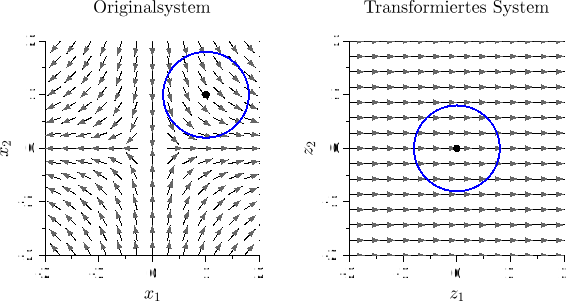
\includegraphics[width=0.95\textwidth]{beispiel_begradigung_nichtruhelage1}
\par\end{centering}
\caption{Phasenportraits von System~(\ref{eq:beispiel-begrad-nichtruhelage})
und dem transformierten System \label{fig:beispiel-begrad-nichtruhelage}}

\end{figure}

Die Vektorfelder $\tfrac{\partial}{\partial z_{1}},\ldots,\tfrac{\partial}{\partial z_{r}}$
aus Satz~\ref{thm:simultane-begradigung-von-VF} können mit den weiteren
Vektor\-feldern $\tfrac{\partial}{\partial z_{r+1}},\ldots,\tfrac{\partial}{\partial z_{n}}$
(als orthogonales Komplement\index{orthogonales Komplement}, siehe
Abschnitt~\ref{sec:Lineare-Algebra}) zu einer Basis des Tangentialraums
ergänzt werden. Diese Tatsache führt zu folgender Erkenntnis:
\begin{corollary}
\label{cor:ergaenzung-einer-involutiven-distribution}Die Distribution~$\Delta$
sei involutiv und im Punkt $p\in\mathcal{M}$ regulär mit $\dim\Delta=r$.
Dann existieren eine Umgebung $\mathcal{U}\subseteq M$ von~$p$
und $n-r$ Vektorfelder $f_{r+1},\ldots,f_{n}:\mathcal{U}\to\R^{n}$,
so dass
\[
\Delta(x)\oplus\spann\left\{ f_{r+1}(x),\ldots,f_{n}(x)\right\} =\R^{n}
\]
für alle $x\in\mathcal{U}$.
\end{corollary}
\begin{svmultproof2}
Auf Basis von Satz~\ref{thm:simultane-begradigung-von-VF} können
die $r$~Vektorfelder, welche die involutive Distribution~$\Delta$
aufspannen, mit einer Transformation~$T$ in die Form $\tfrac{\partial}{\partial z_{1}},\ldots,\tfrac{\partial}{\partial z_{r}}$
überführt werden. Die von den zusätzlichen Vektorfeldern $\tfrac{\partial}{\partial z_{r+1}},\ldots,\tfrac{\partial}{\partial z_{n}}$
aufgespannte Distribution ist involutiv, weil die Vektorfelder konstant
sind. Die Involutivität bleibt wegen Prop.~\ref{pro:Lie-Klammer-und-Push-Forward}
unter Rücktransformation~$S$ erhalten, wobei die Vektor\-felder
$\tfrac{\partial}{\partial z_{j}}$ dann die Form 
\[
f_{j}(x):=\left.S^{\prime}(z)\tfrac{\partial}{\partial z_{j}}\right|_{z=T(x)}
\]
 für $j=r+1,\ldots,n$ annehmen.
\end{svmultproof2}

Nachfolgend geht es um die Frage, welche Auswirkungen die Involutivität
einer Distribution auf den Annihilator hat.
\begin{definition}
\label{def:Integrierbarkeit-Distribution}Eine reguläre Distribution~$\Delta$
mit $\dim\Delta=r$ heißt \emph{integrierbar}\index{Distribution!integrierbare},
wenn es Skalarfelder $\lambda_{1},\ldots,\lambda_{n-r}$ gibt, so
dass 
\begin{equation}
\Delta^{\perp}=\spann\left\{ \d\lambda_{1},\ldots,\d\lambda_{n-r}\right\} .\label{eq:Distr-def-integrierbar}
\end{equation}
Die Besonderheit einer integrierbaren Distribution besteht also demnach
darin, dass der Annihilator nicht von beliebigen Kovektorfeldern aufgespannt
wird, sondern von exakten Differentialen (d.\,h. von Gradienten\index{Gradient}).
\end{definition}
\begin{theorem}
[Satz von Frobenius]\label{thm:Frobenius-lokal}\index{Satz!von Frobenius}Die
Distribution~$\Delta$ sei im Punkt $p\in\mathcal{M}$ regulär.\index{Distribution!reguläre}\index{Distribution!involutive}
In einer geeigneten Umgebung~$\mathcal{U}$ von~$p$ gilt dann:
\[
\Delta\mbox{ ist involutiv}\quad\Longleftrightarrow\quad\Delta\mbox{ ist integrierbar.}
\]
\end{theorem}
\begin{svmultproof2}
Da die Distribution regulär ist, gibt es $r=\dim\Delta$ linear unabhängige
Vektor\-felder $f_{1},\ldots,f_{r}:\mathcal{U}{\to\R}^{n}$ mit $\Delta=\spann\{f_{1},\ldots,f_{r}\}$.

\hinreichend\ Nach Lemma~\ref{lem:Basisdarstellung-involutive-Distribution}
können die Vektorfelder so gewählt werden, dass 
\[
[f_{i},f_{j}]\equiv0\quad\mbox{für}\quad1\leq i,j\leq r.
\]
Nach dem Begradigungssatz~\ref{thm:simultane-begradigung-von-VF}
existiert ein lokaler Diffeomorphismus $z=T(x)$ mit $T=(t_{1},\ldots,t_{n})^{T}$,
so dass
\[
\left.T^{\prime}(x)f_{i}(x)\right|_{x=T^{-1}(z)}=\frac{\partial}{\partial z_{i}}\quad\mbox{für}\quad i=1,\ldots,r.
\]
Dadurch werden die Vektorfelder in Richtung der Einheisvektoren $\tfrac{\partial}{\partial z_{1}},\ldots,\tfrac{\partial}{\partial z_{r}}$
ausgerichtet. Die Kovektoren $\d z_{r+1},\ldots,\d z_{n}$ der dualen
Basis sind dazu orthogonal, d.\,h. 
\[
\left\langle \d z_{j},\frac{\partial}{\partial z_{i}}\right\rangle =0\quad\mbox{für}\quad\begin{array}{ccl}
i & = & 1,\ldots,r,\\
j & = & r+1,\ldots,n.
\end{array}
\]
Dann gilt
\[
\begin{array}{ccl}
0 & = & \left\langle \d z_{j},\frac{\partial}{\partial z_{i}}\right\rangle \\
 & = & \left\langle \d z_{j},T^{\prime}(x)f_{i}(x)\right\rangle \\
 & = & \left\langle \d z_{j}T^{\prime}(x),f_{i}(x)\right\rangle \\
 & = & \left\langle \d t_{j}(x),f_{i}(x)\right\rangle 
\end{array}
\]
für $i=1,\ldots,r$ und $j=r+1,\ldots,n$, wobei $\d t_{j}$ die $j$-te
Zeile der Jacobi\-matrix~$T^{\prime}$ darstellt. Die Kovektorfelder
$\d t_{r+1},\ldots,\d t_{n}$ sind also orthogonal zu den die Distribution
aufspannenden Vektorfeldern $f_{1},\ldots,f_{r}$ und damit Elemente
des Annihilators~$\Delta^{\perp}$. Aufgrund des Begradigungssatzes
ist~$T$ ein Diffeomorphismus, insbesondere ist $T^{\prime}(p)$
regulär. Damit sind die Zeilen $\d t_{r+1},\ldots,\d t_{n}$ in der
Umgebung von~$p$ linear unabhängig. Die Differentiale $\d\lambda_{k}$
mit $\lambda_{k}=t_{r+k}$ für $k=1,\ldots,n-r$ spannen folglich~$\Delta^{\perp}$
auf, d.\,h. es gilt~(\ref{eq:Distr-def-integrierbar}). Damit ist~$\Delta$
integrierbar.

\notwendig\ Die Distribution~$\Delta$ sei integrierbar, d.\,h.
es gibt Skalarfelder $\lambda_{1},\ldots,\lambda_{n-r}$ mit~(\ref{eq:Distr-def-integrierbar}).
Daher gilt 
\[
L_{f_{i}}\lambda_{j}=\left\langle \d\lambda_{j},f_{i}\right\rangle =0\quad\mbox{für}\quad\begin{array}{ccl}
i & = & 1,\ldots,r,\\
j & = & r+1,\ldots,n.
\end{array}
\]
Weitere Lie-Ableitungen entlang~$f_{k}$ sind ebenfalls Null: 
\[
L_{f_{k}}L_{f_{i}}\lambda=\langle\underbrace{\d L_{f_{i}}\lambda_{j}}_{{\displaystyle =0}},f_{k}\rangle=0\quad\mbox{für}\quad1\leq i,k\leq r.
\]
Daher gilt 
\[
L_{[f_{i},f_{k}]}\lambda_{j}=L_{f_{i}}L_{f_{k}}\lambda_{j}-L_{f_{k}}L_{f_{i}}\lambda_{j}=0.
\]
Für $j=1,\ldots,n-r$ erhält man 
\[
\left(\begin{array}{c}
L_{[f_{i},f_{k}]}\lambda_{1}\\
\vdots\\
L_{[f_{i},f_{k}]}\lambda_{n-r}
\end{array}\right)=\left(\begin{array}{c}
\d\lambda_{1}\\
\vdots\\
\d\lambda_{n-r}
\end{array}\right)[f_{i},f_{k}]=0.
\]
Die Kovektorfelder $\d\lambda_{1},\ldots,\d\lambda_{n-r}$ spannen
laut Annahme den Annihilator von~$\Delta$ auf. Die Lie-Klammern
$[f_{i},f_{k}]$ stehen senkrecht auf der Basis von~$\Delta^{\perp}$
und gehören damit zu~$\Delta$, d.\,h. $[f_{i},f_{k}]\in\Delta$.
Also ist~$\Delta$ involutiv.
\end{svmultproof2}

\begin{example}
\label{exa:Frobenius1}Man betrachte die von den Vektorfeldern 
\[
f_{1}(x)=-2x_{2}\frac{\partial}{\partial x_{3}}\quad\text{und}\quad f_{2}(x)=-2x_{2}\frac{\partial}{\partial x_{1}}+2x_{1}\frac{\partial}{\partial x_{2}}
\]
auf der Menge $\mathcal{M}=\left\{ x\in\R^{3};\;x_{1}\neq0\wedge x_{2}\neq0\right\} $
aufgespannte Distribution $\Delta=\spann\{f_{1},f_{2}\}.$ Diese Distribution~$\Delta$
kann man auch in der Form 
\[
\Delta(x)=\im\,F(x)\quad\text{mit}\quad F(x)=\left(f_{1}(x),f_{2}(x)\right)=\left(\begin{array}{cc}
0 & -2x_{2}\\
0 & \phantom{{-}}2x_{1}\\
-2x_{2} & 0
\end{array}\right)
\]
beschreiben, wobei die Matrix $F(x)$ für alle $x\in\mathcal{M}$
den Rang~$2$ aufweist. Folglich ist die Distribution regulär mit
$\dim\Delta=2$. Außerdem ist die Distribution wegen 
\[
[f_{1},f_{2}](x)=4x_{1}\frac{\partial}{\partial x_{3}}=-2\frac{x_{1}}{x_{2}}(-2x_{2})\frac{\partial}{\partial x_{3}}=-2\frac{x_{1}}{x_{2}}f_{1}(x)\in\Delta(x)
\]
involutiv (vgl. Lemma~\ref{lem:Involutivitaetstest-mit-basis}),
so dass die Voraussetzung von Satz~\ref{thm:Frobenius-lokal} erfüllt
sind. Eine mögliche Basis des Annihilators lässt sich mit \textsc{Maxima}
berechnen:

\begin{maxima}\noindent
%%%%%%%%%%%%%%%
%%% INPUT:
\begin{minipage}[t]{8ex}
\color{red}\bf
\begin{verbatim}
(%i1) 
\end{verbatim}
\end{minipage}
\begin{minipage}[t]{\textwidth}
\color{blue}
\begin{verbatim}
load(eigen)$
\end{verbatim}
\end{minipage}

\smallskip

\noindent
%%%%%%%%%%%%%%%
%%% INPUT:
\begin{minipage}[t]{8ex}
\color{red}\bf
\begin{verbatim}
(%i2) 
\end{verbatim}
\end{minipage}
\begin{minipage}[t]{\textwidth}
\color{blue}
\begin{verbatim}
f1:columnvector([0,0,-2*x2])$
f2:columnvector([-2*x2,2*x1,0])$
F:addcol(f1,f2);
\end{verbatim}
\end{minipage}
%%% OUTPUT:
\begin{math}\displaystyle
\parbox{8ex}{\color{labelcolor}(\%o4) }
\begin{pmatrix}0 & -2\,x2\cr 0 & 2\,x1\cr -2\,x2 & 0\end{pmatrix}
\end{math}
%%%%%%%%%%%%%%%


\noindent
%%%%%%%%%%%%%%%
%%% INPUT:
\begin{minipage}[t]{8ex}
\color{red}\bf
\begin{verbatim}
(%i5) 
\end{verbatim}
\end{minipage}
\begin{minipage}[t]{\textwidth}
\color{blue}
\begin{verbatim}
A:nullspace(transpose(F));
\end{verbatim}
\end{minipage}
%%% OUTPUT:
\begin{math}\displaystyle
Proviso: \mathrm{notequal}\left( -2\,x2,0\right) \;\wedge\; \mathrm{notequal}\left( 4\,{x2}^{2},0\right) 
\end{math}

\noindent
\begin{math}\displaystyle
\parbox{8ex}{\color{labelcolor}(\%o5) }
\mathrm{span}\left( \begin{pmatrix}4\,x1\,x2\cr 4\,{x2}^{2}\cr 0\end{pmatrix}\right) 
\end{math}
%%%%%%%%%%%%%%%

\end{maxima}

Das Kovektorfeld $\omega(x)=4x_{1}x_{2}\d x_{1}+4x_{2}^{2}\d x_{2}$
spannt folglich den Annihilator auf: $\Delta^{\perp}=\spann\{\omega\}$.
Aus dem Poincaréschen Lemma (Lemma~\ref{lem:poincare}) folgt wegen
\[
\frac{\partial\omega_{1}}{\partial x_{2}}=4x_{1}\neq\frac{\partial\omega_{2}}{\partial x_{1}}=0
\]
die Aussage, dass $\omega$ nicht exakt ist. Allerdings kann man mit
dem \emph{integrierenden Faktor}\index{integrierender Faktor} $\mu(x)=1/(4x_{2})$
das Kovektorfeld~$\omega$ in das exakte Kovektorfeld 
\[
\D\hbar(x)=\varpi(x):=\mu(x)\cdot\omega(x)=x_{1}\D x_{1}+x_{2}\D x_{2}
\]
mit dem Potential $\hbar(x)=\half x_{1}^{2}+\half x_{2}^{2}$ überführen.
Der Annihilator $\Delta^{\perp}=\spann\{\D\hbar\}$ wird also von
dem Gradienten $\D\hbar$ aufgespannt.
\end{example}

In Analogie zu Korollar~\ref{cor:ergaenzung-einer-involutiven-distribution}
ist auf Basis von Satz~\ref{thm:Frobenius-lokal} folgende Aussage
möglich:
\begin{corollary}
\label{cor:ergaenzung-einer-kodistribution-integrierbar}Gegeben seien
die Skalarfelder $\lambda_{1},\ldots,\lambda_{n-r}:\mathcal{M}\to\R$,
so dass die Kodistribution
\[
\Omega=\spann\left\{ \d\lambda_{1},\ldots,\d\lambda_{n-r}\right\} 
\]
im Punkt $p\in\mathcal{M}$ regulär ist mit $\dim\Omega=n-r$. Dann
existieren eine Umgebung $\mathcal{U}\subseteq\mathcal{M}$ und $r$
weitere Skalarfelder $\lambda_{n-r+1},\ldots,\lambda_{n}:\mathcal{U}\to\R$,
so dass 
\[
\Omega(x)\oplus\spann\left\{ \d\lambda_{n-r+1},\ldots,\d\lambda_{n}\right\} =(\R^{n})^{*}
\]
für alle $x\in\mathcal{U}$ gilt und die Abbildung $\Lambda(x)=(\lambda_{1}(x),\ldots,\lambda_{n}(x))^{T}$
in einer Umgebung von~$p$ ein lokaler Diffeomeorphismus ist.
\end{corollary}
\begin{svmultproof2}
Der Annihilator $\Delta:=\Omega^{\perp}$ ist eine involutive Distribution
(Satz~\ref{thm:Frobenius-lokal}). Die Konstruktion der Skalarfelder
$\lambda_{1},\ldots,\lambda_{n-r}$ erfolgt im Beweis von Satz~\ref{thm:Frobenius-lokal}
über die Koordinatentransformation des Begradigungssatzes (Satz~\ref{thm:simultane-begradigung-von-VF}).
Die Kovektorfelder $\d\lambda_{1},\ldots,\d\lambda_{n-r}$ entsprechen
in den transformierten Koordinaten den Elementen $\d z_{r+1},\ldots,\d z_{n}$.
Mit $\d z_{1},\ldots,\d z_{r}$ erfolgt die Ergänzung zu einer Basis
des Dualraums~$(\R^{n})^{*}$. Die Basisergänzung nutzt die Gradienten
der linearen Abbildungen $z\mapsto z_{j}$ für $j=1,\ldots,r$. Die
Anwendung der Transformation~$T$ liefert die gesuchten Skalarfelder
$\lambda_{n-r+1}=t_{1},\ldots,\lambda_{n}=t_{r}$.
\end{svmultproof2}

Ist eine Distribution nicht involutiv, so kann man sie durch Hinzunahme
weiterer Vektorfelder zu einer involutiven Distribution vervollständigen.
Der \emph{involutiver Abschluss}\index{involutiver Abschluss} $\inv(\Delta)$
einer Distribution $\Delta$ ist die kleinste involutive Distribution,
die $\Delta$ enthält, d.\,h. $\Delta\subseteq\inv(\Delta)$. Den
involutiven Abschluss bildet man, indem man zu einer gegebenen Distribution
$\Delta$ solange Lie-Klammern der beteiligten Vektorfelder hinzufügt
(d.\,h. für alle $f,g\in\Delta$ bildet man $\Delta+\spann\{[f,g]\}$
usw.), bis die resultierende Distribution involutiv ist. Eine einfache
Prototypimplementierung in Maxima ist Alg.~\ref{alg:Involutiver-Abschluss}
zu entnehmen, wobei die Nutzung nachfolgend an einem Beispiel illustriert
wird. Ist die Distribution $\Delta$ selber bereits involutiv, so
gilt $\Delta=\inv(\Delta)$. 

\begin{algorithm}
\noindent
%%%%%%%%%%%%%%%
%%% INPUT:
%\begin{minipage}[t]{8ex}
%\color{red}\bf
%\begin{verbatim}
%(%i12) 
%\end{verbatim}
%\end{minipage}
\begin{minipage}[t]{\textwidth}
\color{blue}
\begin{verbatim}
InvolutiveClosure(L,x):=block([flag,F,G,i,j,r,n],
    F:apply('matrix,L),
    F:transpose(F),
    flag:true,
    while flag do (
        flag:false,
        [n,r]:matrix_size(F),
        for i:1 thru r do 
            for j:i+1 thru r do block([f1,f2],
                f1:list_matrix_entries(col(F,i)),
                f2:list_matrix_entries(col(F,j)),
                G:addcol(F,LieBracket(f1,f2,x)),
                if rank(F)<rank(G) then (
                    F:copy(G),
                    flag:true
                )       
        )
    ),
    makelist(makelist(F[i,j],i,1,n),j,1,r)
)$
\end{verbatim}
\end{minipage}


\caption{Berechnung des involutiven Abschlusses einer Distribution\label{alg:Involutiver-Abschluss}}

\end{algorithm}

\begin{example}
\label{exa:Roboter-involutiver-Abschluss}Die von den Vektorfeldern~$f_{1}$
und~$f_{2}$ des mobilen Roboters aus den Beispielen~\ref{exa:Lie-Vektorfeld-Roboter}
und~\ref{exa:Roboter-Test-Involutivitaet} aufgespannte Distribution
$\Delta=\spann\{f_{1},f_{2}\}$ ist nicht involutiv. Für den involutiven
Abschluss ist mindestens die Lie-Klammer $[f_{1},f_{2}]$ einzubeziehen.
Die Vektorfelder $f_{1}$, $f_{2}$, $[f_{1},f_{2}]$ sind linear
unabhängig und spannen den gesamten Vektorraum auf, d.\,h. 
\begin{equation}
\Delta(x)+\spann\left\{ [f,g](x)\right\} =\spann\left\{ f(x),g(x),[f,g](x)\right\} =\R^{3},\label{eq:Roboter-Dist-involutiver-Abschluss}
\end{equation}
siehe Beispiel~\ref{exa:Roboter-Test-Involutivitaet}. Damit ist~(\ref{eq:Roboter-Dist-involutiver-Abschluss})
involutiv, d.\,h. $\inv(\Delta)=\spann\{f_{1},f_{2},[f_{1},f_{2}]\}$.
Dieses Resultat erhält man auch mit \textsc{Maxima}:

\begin{maxima}\noindent
%%%%%%%%%%%%%%%
%%% INPUT:
\begin{minipage}[t]{8ex}
\color{red}\bf
\begin{verbatim}
(%i6) 
\end{verbatim}
\end{minipage}
\begin{minipage}[t]{\textwidth}
\color{blue}
\begin{verbatim}
f1:[sin(x3),cos(x3),0];
f2:[0,0,1];
x:[x1,x2,x3];
\end{verbatim}
\end{minipage}
%%% OUTPUT:
\begin{math}\displaystyle
\parbox{8ex}{\color{labelcolor}(\%o4) }
[\mathrm{sin}\left( x3\right) ,\mathrm{cos}\left( x3\right) ,0]
\end{math}

\noindent
\begin{math}\displaystyle
\parbox{8ex}{\color{labelcolor}(\%o5) }
[0,0,1]
\end{math}

\noindent
\begin{math}\displaystyle
\parbox{8ex}{\color{labelcolor}(\%o6) }
[x1,x2,x3]
\end{math}
%%%%%%%%%%%%%%%


\noindent
%%%%%%%%%%%%%%%
%%% INPUT:
\begin{minipage}[t]{8ex}
\color{red}\bf
\begin{verbatim}
(%i7) 
\end{verbatim}
\end{minipage}
\begin{minipage}[t]{\textwidth}
\color{blue}
\begin{verbatim}
InvolutiveClosure([f1,f2],x);
\end{verbatim}
\end{minipage}
%%% OUTPUT:
\begin{math}\displaystyle
\parbox{8ex}{\color{labelcolor}(\%o7) }
[[\mathrm{sin}\left( x3\right) ,\mathrm{cos}\left( x3\right) ,0],[0,0,1],[-\mathrm{cos}\left( x3\right) ,\mathrm{sin}\left( x3\right) ,0]]
\end{math}
%%%%%%%%%%%%%%%
\end{maxima}
\end{example}

\section{Differentialformen\label{sec:Differentialformen}}

Dieser Abschnitt gibt eine kurze Einführung in das Gebiet der Differentialformen.
Ähnliche Kurzdarstellungen findet der Leser auch in~\cite{zeidler2013tb4}
und~\cite[Kapitel~1]{taschner2015band3}. Detailliertere Einführungen
sind beispielsweise in \cite[Kapitel~7]{arnold1989}, \cite{kerner2007}
oder \cite[Anhang~B]{knauf2012} zu finden. Für weiterführende Aussagen
sei auf~\cite{agricola2001,jaenich2005,lee2006} sowie~\cite[Kapitel~12]{sastry1999}
verwiesen.

\medskip{}

In Abschnitt~\ref{sec:Felder-und-Ableitungen} wurden Differentialformen
ersten Grades als auf einer offenen Menge $\mathcal{M}\subseteq\R^{n}$
definierte Kovektorfelder in der Form 
\[
\omega(x)=\omega_{1}(x)\d x_{1}+\cdots+\omega_{n}(x)\d x_{n}
\]
mit den Skalarfeldern $\omega_{i}:\mathcal{M}\to\R$ als Komponenten
und den Basiselementen $\d x_{i}$ für die eindimensionale Indexmenge
$i=1,\ldots n$ eingeführt. Unter einer \emph{Differentialform $k$-ten
Grades}\index{Differentialform!$k$-ten Grades} (kurz \emph{$k$-Form})
versteht man einen Ausdruck der Gestalt 
\begin{equation}
\omega(x)=\sum\omega_{i_{1}\cdots i_{k}}(x)\ \d x_{i_{1}}\wedge\ldots\wedge\d x_{i_{k}}\label{eq:Differentialform-Grad-k}
\end{equation}
mit Komponenten $\omega_{i_{1}\cdots i_{k}}:\mathcal{M}\to\R$ und
(zunächst formalen) Elementen
\begin{equation}
\d x_{i_{1}}\wedge\ldots\wedge\d x_{i_{k}},\label{eq:Basis-k-Form}
\end{equation}
die jeweils über $k$ Indizes $i_{1},\ldots,i_{k}$ adressiert werden.
Jedes Element~(\ref{eq:Basis-k-Form}) kann man als spezielle $k$-Form~(\ref{eq:Differentialform-Grad-k})
auffassen, bei der die Komponente zu den Indizes $i_{1},\ldots,i_{k}$
den Wert Eins und alle sonstigen Komponenten den Wert Null annehmen.
Differentialformen sind \emph{alternierend} (\emph{schiefsymmetrisch}
oder \emph{antisymmetrisch}), d.\,h. beim Vertauschen von genau zwei
Indizes~$i_{j}$ und~$i_{\ell}$ in~(\ref{eq:Basis-k-Form}) wechselt
auch das Vorzeichen: 
\begin{gather}
\d x_{i_{1}}\wedge\ldots\wedge\d x_{i_{j}}\wedge\ldots\wedge\d x_{i_{\ell}}\wedge\ldots\wedge\d x_{i_{k}}\nonumber \\
=-\d x_{i_{1}}\wedge\ldots\wedge\d x_{i_{\ell}}\wedge\ldots\wedge\d x_{i_{j}}\wedge\ldots\wedge\d x_{i_{k}}.\label{eq:k-Form-alternierende-Basiselemente}
\end{gather}
Daraus folgt zusätzlich, dass bei zwei übereinstimmenden Indizes der
entsprechende Term verschwindet: 
\begin{equation}
\d x_{i_{1}}\wedge\ldots\wedge\d x_{i_{j}}\wedge\ldots\wedge\d x_{i_{j}}\wedge\ldots\wedge\d x_{i_{k}}=0.\label{eq:k-Form-Null-bei-gleichen-Indizes}
\end{equation}
Wegen~(\ref{eq:k-Form-alternierende-Basiselemente}) und~(\ref{eq:k-Form-Null-bei-gleichen-Indizes})
genügt es, für die Darstellung einer $k$-Form nach Gl.~(\ref{eq:Differentialform-Grad-k})
über die sortierten Indizes 
\begin{equation}
1\leq i_{1}<\cdots<i_{j}<\cdots<i_{k}\leq n\label{eq:k-Form-Numerierung-sortiert}
\end{equation}
zu summieren.

Eine $k$-Form~(\ref{eq:Differentialform-Grad-k}) heißt \emph{differenzierbar},
wenn alle Komponenten $\omega_{i_{1}\cdots i_{k}}:\mathcal{M}\to\R$
differenzierbar sind. In analoger Weise übertragen wir die Begriffe
\emph{hinreichend glatt}, \emph{glatt} und \emph{analytisch} auf Differentialformen
(vgl. Abschnitt~\ref{sec:Vektorfelder-und-Fluesse}). Wir gehen nachfolgend
davon aus, dass die betrachteten Differentialformen hinreichend glatt
sind. Die Menge der auf~$\mathcal{M}$ definierten $k$-Formen bildet
einen Vektorraum\footnote{Die Menge der $k$-Formen bildet einerseits einen reellen Vektorraum,
der aufgrund der funktionswertigen Koeffizienten für $k\in\{0,\ldots,n\}$
unendlichdimensional ist.  Für die nachfolgenden Dimensionsangaben
betrachten wir die $k$-Formen als Vektorraum über den meromorphen
Funktionen. Das bedeutet, dass die Koeffizientenfunktionen mit Ausnahme
von isolierten Singularitäten analytisch sind.}, den wir im Folgenden mit $\Omega^{k}(\mathcal{M})$ bezeichnen.
Dabei fassen wir $\Omega^{0}(\mathcal{M})$ als die Menge der Skalarfelder
und $\Omega^{1}(\mathcal{M})$ als die Menge der Kovektorfelder mit
dem Definitionsbereich~$\mathcal{M}$ auf. Die Elemente~(\ref{eq:Basis-k-Form}),
welche der Ungleichung~(\ref{eq:k-Form-Numerierung-sortiert}) genügen,
sind eine Basis dieses Vektorraums. Für $k\in\{0,\ldots,n\}$ besteht
diese Basis aus ${n \choose k}=\frac{n!}{k!\,(n-k)!}$ Elementen.
Im Fall $k=n$ erhält man genau ein Basiselement $\d x_{1}\wedge\ldots\wedge\d x_{n}$.
Der zugehörige Vektorraum besitzt daher die Dimension ${n \choose n}=1$,
weshalb man die Elemente von $\Omega^{n}(\mathcal{M})$ mitunter auch
als \emph{Pseudoskalare}\index{Pseudoskalar} bezeichnet~\cite{hestenes1999}.
Für $k>n$ stimmen mindestens zwei der bei~(\ref{eq:Basis-k-Form})
auftretenden Indizes $i_{1},\ldots,i_{k}$ überein, so dass dann wegen
Gl.~(\ref{eq:k-Form-Null-bei-gleichen-Indizes}) jede $k$-Form Null
ist, womit der zugehörige Vektorraum die Dimension Null aufweist.
Die direkte Summe aller $k$-Formen für $k=0,\ldots,n$ bildet die
\emph{äußere Algebra}\index{außere Algebra@äußere Algebra}\index{Algebra!außere@äußere}
oder \emph{Graßmann-Algebra}\index{Graßmann-Algebra}\index{Algebra!Graßmann-}
$\Omega(\mathcal{M}):=\Omega^{0}(\mathcal{M})\oplus\cdots\oplus\Omega^{n}(\mathcal{M})$,
welche die Dimension $\sum_{k=0}^{n}{n \choose k}=2^{n}$ besitzt.
\begin{example}
Für $\mathcal{M}=\R^{3}$ sind $k$-Formen nur für $k=0,\ldots,3$
relevant. Diese haben folgende Form:
\begin{align*}
0\text{-Formen:}\qquad & \omega(x)\\
1\text{-Formen:}\qquad & \omega_{1}(x)\,\d x_{1}+\omega_{2}(x)\,\d x_{2}+\omega_{3}(x)\,\d x_{3}\\
2\text{-Formen:}\qquad & \omega_{12}(x)\,\d x_{1}\wedge\d x_{2}+\omega_{13}(x)\,\d x_{1}\wedge\d x_{3}+\omega_{23}(x)\,\d x_{2}\wedge\d x_{3}\\
3\text{-Formen:}\qquad & \omega_{123}(x)\,\d x_{1}\wedge\d x_{2}\wedge\d x_{3}
\end{align*}
\end{example}
\medskip{}

Nachfolgend werden die wichtigsten Operationen für das Rechnen mit
Differentialformen eingeführt. Die angegebenen Berechnungen können
im Computer-Algebra-System \textsc{Maxima} mit der \texttt{cartan}-Toolbox
von F.~B. Estabrook and H.~D. Wahlquist durchgeführt werden. Alternativ
kann man die deutlich umfangreicheren Tensor-Toolboxen (\texttt{itensor},
\texttt{ctensor}, \texttt{atensor}) von Viktor T. Toth einsetzen~\cite{toth2005}.

Die Addition ist nur zwischen Differentialformen gleichen Grades zugelassen.
Für zwei Differentialformen $\omega,\eta\in\Omega^{k}(\mathcal{M})$
mit
\begin{eqnarray}
\omega(x) & = & \sum_{i_{1}<\cdots<i_{k}}\omega_{i_{1}\cdots i_{k}}(x)\ \d x_{i_{1}}\wedge\ldots\wedge\d x_{i_{k}}\label{eq:k-form-omega}\\
\eta(x) & = & \sum_{i_{1}<\cdots<i_{k}}\eta_{i_{1}\cdots i_{k}}(x)\ \d x_{i_{1}}\wedge\ldots\wedge\d x_{i_{k}}\label{eq:k-form-eta}
\end{eqnarray}
vom Grad~$k$ ist die Summe komponentenweise durch
\begin{equation}
(\omega+\eta)(x)=\sum_{i_{1}<\cdots<i_{k}}\left(\omega_{i_{1}\cdots i_{k}}(x)+\eta_{i_{1}\cdots i_{k}}(x)\right)\ \d x_{i_{1}}\wedge\ldots\wedge\d x_{i_{k}}\label{eq:k-form-summe}
\end{equation}
definiert. Für die Multiplikation steht das \emph{Keilprodukt}\index{Keilprodukt}\index{Produkt!Keil-}
(\emph{Dachprodukt}\index{Dachprodukt}\index{Produkt!Dach-}, \emph{äußere
Produkt}\index{außeres Produkt@äußeres Produkt}\index{Produkt!außeres@äußeres},
engl. \emph{wegde product}) zur Verfügung, welches zwischen zwei Differentialformen
beliebigen Grades möglich ist. Das Produkt einer $k$-Form~(\ref{eq:k-form-omega})
mit einer $\ell$-Form
\[
\eta(x)=\sum_{j_{1}<\cdots<j_{\ell}}\eta_{j_{1}\cdots j_{\ell}}(x)\ \d x_{j_{1}}\wedge\ldots\wedge\d x_{j_{\ell}}
\]
ist eine $(k+\ell)$-Form, die sich komponentenweise durch
\begin{equation}
(\omega\wedge\eta)(x)=\!\!\!\sum\limits _{{i_{1}<\cdots<i_{k}\atop j_{1}<\cdots<j_{\ell}}}\omega_{i_{1}\cdots i_{k}}(x)\cdot\eta_{j_{1}\cdots j_{\ell}}(x)\,\d x_{i_{1}}\wedge\ldots\wedge\d x_{i_{k}}\wedge\d x_{j_{1}}\wedge\ldots\wedge\d x_{j_{\ell}}\label{eq:k-l-form-produkt}
\end{equation}
ergibt. Durch Anwendung von~(\ref{eq:k-Form-alternierende-Basiselemente})
und~(\ref{eq:k-Form-Null-bei-gleichen-Indizes}) überführt man das
Produkt~(\ref{eq:k-l-form-produkt}) in die Form mit sortierten Indizes.
Das Produkt einer $k$-Form mit einer $0$-Form $h\in\Omega^{0}(\mathcal{M})$
(also mit einem Skalarfeld $h:\mathcal{M}\to\R$) entspricht der skalaren
Multiplikation, so dass das Skalarfeld in alle Komponenten hineingezogen
wird:
\begin{equation}
(h\wedge\omega)(x)=\sum_{i_{1}<\cdots<i_{k}}h(x)\cdot\omega_{i_{1}\cdots i_{k}}(x)\ \d x_{i_{1}}\wedge\ldots\wedge\d x_{i_{k}}.\label{eq:produkt-mit-nullform}
\end{equation}

\begin{example}
\label{exa:Formen-Kleinprodukt}Auf $\mathcal{M}=\R^{3}$ betrachte
man die drei $1$-Formen 
\begin{eqnarray*}
\omega & = & \omega_{1}\,\d x_{1}+\omega_{2}\,\d x_{2}+\omega_{3}\,\d x_{3}\\
\eta & = & \eta_{1}\,\d x_{1}+\eta_{2}\,\d x_{2}+\eta_{3}\,\d x_{3}\\
\sigma & = & \sigma_{1}\,\d x_{1}+\sigma_{2}\,\d x_{2}+\sigma_{3}\,\d x_{3}.
\end{eqnarray*}
Das äußere Produkt der $1$-Formen~$\omega$ und~$\eta$ ist die
$2$-Form 
\begin{eqnarray}
\omega\wedge\eta & = & \phantom{+}\omega_{1}\eta_{1}\,\cancel{\d x_{1}\wedge\d x_{1}}+\omega_{1}\eta_{2}\,\d x_{1}\wedge\d x_{2}+\omega_{1}\eta_{3}\,\d x_{1}\wedge\d x_{3}\nonumber \\
 &  & +\omega_{2}\eta_{1}\,\d x_{2}\wedge\d x_{1}+\omega_{2}\eta_{2}\,\cancel{\d x_{2}\wedge\d x_{2}}+\omega_{2}\eta_{3}\,\d x_{2}\wedge\d x_{3}\nonumber \\
 &  & +\omega_{3}\eta_{1}\,\d x_{3}\wedge\d x_{1}+\omega_{3}\eta_{2}\,\d x_{3}\wedge\d x_{2}+\omega_{3}\eta_{3}\,\cancel{\d x_{3}\wedge\d x_{3}}\nonumber \\
 & = & \phantom{+}\left(\omega_{1}\eta_{2}-\omega_{2}\eta_{1}\right)\d x_{1}\wedge\d x_{2}+\left(\omega_{1}\eta_{3}-\omega_{3}\eta_{1}\right)\d x_{1}\wedge\d x_{3}\nonumber \\
 &  & +\left(\omega_{2}\eta_{3}-\omega_{3}\eta_{2}\right)\d x_{2}\wedge\d x_{3}.\label{eq:bsp-produkt-2-1-Formen}
\end{eqnarray}
Multipliziert man dieses Ergebnis zusätzlich von rechts mit der dritten
$1$-Form~$\sigma$, so erhält man die $3$-Form
\begin{eqnarray}
\omega\wedge\eta\wedge\sigma & = & \left(\omega_{1}\eta_{2}\sigma_{3}-\omega_{1}\eta_{3}\sigma_{2}+\omega_{2}\eta_{3}\sigma_{1}-\omega_{2}\eta_{1}\sigma_{3}\right.\nonumber \\
 &  & \left.+\,\omega_{3}\eta_{1}\sigma_{2}-\omega_{3}\eta_{2}\sigma_{1}\right)\d x_{1}\wedge\d x_{2}\wedge\d x_{3}.\label{eq:bsp-produkt-3-1-Formen}
\end{eqnarray}
Diese Resultate lassen sich mit der \texttt{cartan}-Toolbox von \textsc{Maxima}
verifizieren. Mit \verb|init_cartan| wird die Basis des Kotangentialraums
angelegt. Für das Keilprodukt steht der Operator ,,$\sim$`` zur
Verfügung.

\begin{maxima}\noindent
%%%%%%%%%%%%%%%
%%% INPUT:
\begin{minipage}[t]{8ex}\color{red}\bf
\begin{verbatim}
(%i2) 
\end{verbatim}
\end{minipage}
\begin{minipage}[t]{\textwidth}\color{blue}
\begin{verbatim}
load(basic)$
if get('cartan,'version)=false then load(cartan)$
\end{verbatim}
\end{minipage}

\smallskip

\noindent
%%%%%%%%%%%%%%%
%%% INPUT:
\begin{minipage}[t]{8ex}\color{red}\bf
\begin{verbatim}
(%i3) 
\end{verbatim}
\end{minipage}
\begin{minipage}[t]{\textwidth}\color{blue}
\begin{verbatim}
init_cartan([x1,x2,x3]);
\end{verbatim}
\end{minipage}
%%% OUTPUT:
\begin{math}\displaystyle
\parbox{8ex}{\color{labelcolor}(\%o3) }
[dx1,dx2,dx3]
\end{math}
%%%%%%%%%%%%%%%


\noindent
%%%%%%%%%%%%%%%
%%% INPUT:
\begin{minipage}[t]{8ex}\color{red}\bf
\begin{verbatim}
(%i6) 
\end{verbatim}
\end{minipage}
\begin{minipage}[t]{\textwidth}\color{blue}
\begin{verbatim}
ω:ω1*dx1+ω2*dx2+ω3*dx3;
η:η1*dx1+η2*dx2+η3*dx3;
σ:σ1*dx1+σ2*dx2+σ3*dx3;
\end{verbatim}
\end{minipage}
%%% OUTPUT:
\begin{math}\displaystyle
\parbox{8ex}{\color{labelcolor}(\%o4) }
dx3\,\omega3+dx2\,\omega2+dx1\,\omega1
\end{math}

\noindent
\begin{math}\displaystyle
\parbox{8ex}{\color{labelcolor}(\%o5) }
dx3\,\eta3+dx2\,\eta2+dx1\,\eta1
\end{math}

\noindent
\begin{math}\displaystyle
\parbox{8ex}{\color{labelcolor}(\%o6) }
dx3\,\sigma3+dx2\,\sigma2+dx1\,\sigma1
\end{math}
%%%%%%%%%%%%%%%


\noindent
%%%%%%%%%%%%%%%
%%% INPUT:
\begin{minipage}[t]{8ex}
\color{red}\bf
\begin{verbatim}
(%i7) 
\end{verbatim}
\end{minipage}
\begin{minipage}[t]{\textwidth}
\color{blue}
\begin{verbatim}
facsum(ω ~ η,dx1,dx2,dx3);
\end{verbatim}
\end{minipage}
%%% OUTPUT:
\begin{math}\displaystyle
\parbox{8ex}{\color{labelcolor}(\%o7) }
-dx2dx3( \eta2\omega3-\eta3\omega2) -dx1dx3( \eta1\omega3-\eta3\omega1) -dx1dx2( \eta1\omega2-\eta2\omega1) 
\end{math}
%%%%%%%%%%%%%%%


\noindent
%%%%%%%%%%%%%%%
%%% INPUT:
\begin{minipage}[t]{8ex}
\color{red}\bf
\begin{verbatim}
(%i8) 
\end{verbatim}
\end{minipage}
\begin{minipage}[t]{\textwidth}
\color{blue}
\begin{verbatim}
factor(ω ~ η ~ σ);
\end{verbatim}
\end{minipage}
%%% OUTPUT:
\begin{math}\displaystyle
\parbox{8ex}{\color{labelcolor}(\%o8) }
dx1dx2dx3( \eta1\sigma2\omega3-\eta2\sigma1\omega3-\eta1\sigma3\omega2+\eta3\sigma1\omega2+\eta2\sigma3\omega1-\eta3\sigma2\omega1) 
\end{math}
%%%%%%%%%%%%%%%
\end{maxima}
\end{example}

Das Keilprodukt unterliegt folgenden Rechenregeln:
\begin{proposition}
\label{prop:Keilprodukt}Gegeben seien die Differentialformen $\omega,\omega_{1},\omega_{2}\in\Omega^{k}(\mathcal{M})$,
$\eta,\eta_{1},\eta_{2}\in\Omega^{\ell}(\mathcal{M})$ und $\sigma\in\Omega^{m}(\mathcal{M})$.
Dann gilt:\begin{subequations}
\begin{eqnarray}
\left(\omega_{1}+\omega_{2}\right)\wedge\eta & = & \omega_{1}\wedge\eta+\omega_{2}\wedge\eta\label{eq:keil-regel1}\\
\omega\wedge\left(\eta_{1}+\eta_{2}\right) & = & \omega\wedge\eta_{1}+\omega\wedge\eta_{2}\label{eq:keil-regel2}\\
\left(\omega\wedge\eta\right)\wedge\sigma & = & \omega\wedge\left(\eta\wedge\sigma\right)\label{eq:keil-assoziativ}\\
\omega\wedge\eta & = & (-1)^{k\ell}\eta\wedge\omega\label{eq:keil-antikommutativ}\\
\omega & = & 1\wedge\omega=\omega\wedge1\label{eq:keil-neutrales-element}
\end{eqnarray}
\end{subequations}
\end{proposition}
Diese Rechenregeln lassen sich unmittelbar auf Basis der komponentenweisen
Definitionen~(\ref{eq:k-form-summe}) und~(\ref{eq:k-l-form-produkt})
beweisen. Mit den Gln.~(\ref{eq:keil-regel1}) und~(\ref{eq:keil-regel2})
ist das Produkt bilinear. Diese zwei Regeln kann man als Distributivgesetze
auffassen. Nach Gl.~(\ref{eq:keil-assoziativ}) ist das Keilprodukt
assoziativ, so dass bei reinen Multiplikationen die Klammern entfallen
können und man $\omega\wedge\eta\wedge\sigma$ schreibt (siehe Gl.~(\ref{eq:bsp-produkt-3-1-Formen})
in Beispiel~\ref{exa:Formen-Kleinprodukt}). Zusätzlich ist das Keilprodukt
nach Gl.~(\ref{eq:keil-antikommutativ}) antikommutativ oder graduiert
kommutativ. Die Zahl~$1$, die zugleich ein spezielles (nämlich konstantes)
Skalarfeld und damit eine $0$-Form ist, bildet entsprechend Gl.~(\ref{eq:keil-neutrales-element})
das neutrale Element (siehe auch Gl.~(\ref{eq:produkt-mit-nullform})).

Ein häufig anzutreffender Spezialfall ist die Produktbildung mehrerer
$1$-Formen. Man betrachte $k$ Kovektorfelder $\omega_{1},\ldots,\omega_{k}\in\Omega^{1}(\mathcal{M})$
der Form $\omega_{j}=\omega_{j1}\d x_{1}+\cdots+\omega_{jn}\d x_{n}$
für $j=1,\ldots,k$. Das Produkt dieser $1$-Formen ist eine $k$-Form,
die sich mit 
\begin{equation}
\omega_{1}\wedge\ldots\wedge\omega_{k}=\sum_{i_{1}<\cdots<i_{k}}\det\left(\begin{array}{ccc}
\omega_{1i_{1}} & \cdots & \omega_{1i_{k}}\\
\vdots & \ddots & \vdots\\
\omega_{ki_{1}} & \cdots & \omega_{ki_{k}}
\end{array}\right)\d x_{i_{1}}\wedge\ldots\wedge\d x_{i_{k}}\label{eq:produkt-k-Einformen}
\end{equation}
berechnen lässt. Mit Gl.~(\ref{eq:produkt-k-Einformen}) kann man
ausgehend von der Basis $\left\{ \d x_{1},\ldots,\d x_{n}\right\} $
des Kotangential\-raums die Basen~(\ref{eq:Basis-k-Form}) der $k$-Formen
für $k=2,\ldots,n$ generieren, wodurch dann auch das Keilprodukt
in der Basis\-darstellung~(\ref{eq:Basis-k-Form}) gerechtfertigt
wird. Für den Spezialfall einer $n$-Form vereinfacht sich Gl.~(\ref{eq:produkt-k-Einformen})
zu
\begin{equation}
\omega_{1}\wedge\ldots\wedge\omega_{n}=\det\left(\begin{array}{ccc}
\omega_{11} & \cdots & \omega_{1n}\\
\vdots & \ddots & \vdots\\
\omega_{n1} & \cdots & \omega_{nn}
\end{array}\right)\d x_{1}\wedge\ldots\wedge\d x_{n}.\label{eq:produkt-n-Einformen}
\end{equation}

\begin{example}
\label{exa:Produkt-1-Formen}Man betrachte die auf $\mathcal{M}=\R^{3}$
definierten $1$-Formen $\omega,\eta,\sigma$ aus Beispiel~\ref{exa:Formen-Kleinprodukt}.
Die Komponenten des Produkts $\omega\wedge\eta$ lassen sich nach
Gl.~(\ref{eq:produkt-k-Einformen}) in Übereinstimmung mit Gl.~(\ref{eq:bsp-produkt-2-1-Formen})
ermitteln:
\[
\begin{array}{llcl}
\d x_{1}\wedge\d x_{2}:\quad & \det\left(\begin{array}{cc}
\omega_{1} & \omega_{2}\\
\eta_{1} & \eta_{2}
\end{array}\right) & = & \omega_{1}\eta_{2}-\omega_{2}\eta_{1},\\
\d x_{1}\wedge\d x_{3}: & \det\left(\begin{array}{cc}
\omega_{1} & \omega_{3}\\
\eta_{1} & \eta_{3}
\end{array}\right) & = & \omega_{1}\eta_{3}-\omega_{3}\eta_{1},\\
\d x_{2}\wedge\d x_{3}: & \det\left(\begin{array}{cc}
\omega_{2} & \omega_{3}\\
\eta_{2} & \eta_{3}
\end{array}\right) & = & \omega_{2}\eta_{3}-\omega_{3}\eta_{2}.
\end{array}
\]
Die Komponente des Produkts $\omega\wedge\eta\wedge\sigma$ zur Basis
$\d x_{1}\wedge\d x_{2}\wedge\d x_{3}$ ergibt sich nach Gl.~(\ref{eq:produkt-n-Einformen})
aus der Determinante
\[
\det\left(\begin{array}{ccc}
\omega_{1} & \omega_{2} & \omega_{3}\\
\eta_{1} & \eta_{2} & \eta_{3}\\
\sigma_{1} & \sigma_{2} & \sigma_{3}
\end{array}\right)=\omega_{1}\eta_{2}\sigma_{3}+\omega_{2}\eta_{3}\sigma_{1}+\omega_{3}\eta_{1}\sigma_{2}-\omega_{1}\eta_{3}\sigma_{2}-\omega_{2}\eta_{1}\sigma_{3}-\omega_{3}\eta_{2}\sigma_{1}.
\]
Dieses Ergebnis stimmt mit Gl.~(\ref{eq:bsp-produkt-3-1-Formen})
aus Beispiel~\ref{exa:Formen-Kleinprodukt} überein.
\end{example}

Aus der Darstellung~(\ref{eq:produkt-k-Einformen}) ergibt sich unmittelbar
folgende Aussage~\cite[Theorem~{12.16}]{sastry1999}:
\begin{proposition}
\label{prop:Lineare-Unabh-Kovektoren-Keil}Die Kovektorfelder $\omega_{1},\ldots,\omega_{k}\in\Omega^{1}(\mathcal{M})$
sind in einem Punkt $p\in\mathcal{M}$ genau dann linear unabhängig,
wenn 
\begin{equation}
\left(\omega_{1}\wedge\ldots\wedge\omega_{k}\right)(p)\neq0.\label{eq:Lineare-Unabh-Kovektoren-Keil}
\end{equation}
\end{proposition}
\begin{svmultproof2}
Die Kovektoren $\omega_{1}(p),\ldots,\omega_{k}(p)\in(\R^{n})^{*}$
sind genau dann linear unabhängig, wenn die Matrix 
\[
W=\left(\begin{array}{c}
\omega_{1}(p)\\
\vdots\\
\omega_{k}(p)
\end{array}\right)=\left(\begin{array}{ccc}
\omega_{11}(p) & \cdots & \omega_{1n}(p)\\
\vdots & \ddots & \vdots\\
\omega_{k1}(p) & \cdots & \omega_{kn}(p)
\end{array}\right)\in\R^{k\times n}
\]
den Rank~$k$, also vollen Zeilenrang, besitzt. Das ist wiederum
genau dann der Fall, wenn es eine $k\times k$-Teilmatrix gibt, deren
Determinante nicht Null ist. Gibt es eine solche Teilmatrix mit Rang~$k$,
dann ist mindestens ein Term der $k$-Form~(\ref{eq:produkt-k-Einformen})
nicht Null. Ist dagegen die Determinante aller $k\times k$-Teilmatrizen
Null, dann ist auch die $k$-Form~(\ref{eq:produkt-k-Einformen})
Null.
\end{svmultproof2}

\medskip{}

Auf der Algebra $\Omega(\mathcal{M})$ ist die \emph{äußere Ableitung}\index{außere Ableitung@äußere Ableitung}\index{Ableitung!außere@äußere}
bzw. das \emph{äußere Differential}\index{außeres Differential@äußeres Differential}\index{Differential!außeres@äußeres}
\[
\d:\Omega^{k}(\mathcal{M})\to\Omega^{k+1}(\mathcal{M})
\]
definiert, welche eine $k$-Form in eine $(k+1)$-Form überführt.
Für eine $0$-Form $h\in\Omega^{0}(\mathcal{M})$ bzw. ein Skalarfeld
$h:\mathcal{M}\to\R$ ist die äußere Ableitung der Gradient (vgl.
Abschnitt~\ref{sec:Felder-und-Ableitungen}): 
\begin{equation}
\d h(x)=\sum_{i=1}^{n}\frac{\partial h(x)}{\partial x_{i}}\,\d x_{i}.\label{eq:formen-ableitung-0-form}
\end{equation}
Für eine $k$-Form $\omega\in\Omega^{k}(\mathcal{M})$ nach Gl.~(\ref{eq:k-form-omega})
ergibt sich die äußere Ableitung komponentenweise aus 
\begin{eqnarray}
\d\omega & = & \sum_{i_{1}<\cdots<i_{k}}\d\omega_{i_{1}\cdots i_{k}}(x)\wedge\d x_{i_{1}}\wedge\ldots\wedge\d x_{i_{k}}\nonumber \\
 & = & \sum_{i_{1}<\cdots<i_{k}}\;\sum_{i=1}^{n}\frac{\partial\omega_{i_{1}\cdots i_{k}}(x)}{\partial x_{i}}\,\d x_{i}\wedge\d x_{i_{1}}\wedge\ldots\wedge\d x_{i_{k}}.\label{eq:formen-def-ableitung}
\end{eqnarray}

\begin{example}
\label{exa:Formen-Ableitung}Auf $\mathcal{M}=\R^{3}$ sei die $1$-Form
\begin{equation}
\omega(x)=\omega_{1}(x)\,\d x_{1}+\omega_{2}(x)\,\d x_{2}+\omega_{3}(x)\,\d x_{3}\label{eq:beispiel-ableitung-omega}
\end{equation}
gegeben. Als äußere Ableitung erhält man die $2$-Form
\begin{eqnarray}
\d\omega(x) & = & \phantom{+}\left(\frac{\partial\omega_{1}(x)}{\partial x_{1}}\d x_{1}+\frac{\partial\omega_{1}(x)}{\partial x_{2}}\d x_{2}+\frac{\partial\omega_{1}(x)}{\partial x_{3}}\d x_{3}\right)\wedge\d x_{1}\nonumber \\
 &  & +\left(\frac{\partial\omega_{2}(x)}{\partial x_{1}}\d x_{1}+\frac{\partial\omega_{2}(x)}{\partial x_{2}}\d x_{2}+\frac{\partial\omega_{3}(x)}{\partial x_{3}}\d x_{3}\right)\wedge\d x_{2}\nonumber \\
 &  & +\left(\frac{\partial\omega_{3}(x)}{\partial x_{1}}\d x_{1}+\frac{\partial\omega_{3}(x)}{\partial x_{2}}\d x_{2}+\frac{\partial\omega_{3}(x)}{\partial x_{3}}\d x_{3}\right)\wedge\d x_{3}\nonumber \\
 & = & \phantom{+}\left(\frac{\partial\omega_{2}(x)}{\partial x_{1}}-\frac{\partial\omega_{1}(x)}{\partial x_{2}}\right)\d x_{1}\wedge\d x_{2}+\left(\frac{\partial\omega_{3}(x)}{\partial x_{1}}-\frac{\partial\omega_{1}(x)}{\partial x_{3}}\right)\d x_{1}\wedge\d x_{3}\nonumber \\
 &  & +\left(\frac{\partial\omega_{3}(x)}{\partial x_{2}}-\frac{\partial\omega_{2}(x)}{\partial x_{3}}\right)\d x_{2}\wedge\d x_{3},\label{eq:beispiel-ableitung-domega}
\end{eqnarray}
wobei die auftretenden Terme entsprechend Gln.~(\ref{eq:k-Form-alternierende-Basiselemente})
und~(\ref{eq:k-Form-Null-bei-gleichen-Indizes}) vereinfacht wurden.
Die Ableitung der $2$-Form 
\[
\eta(x)=\eta_{12}(x)\,\d x_{1}\wedge\d x_{2}+\eta_{13}\,\d x_{1}\wedge\d x_{3}+\eta_{23}\,\d x_{2}\wedge\d x_{3}
\]
ist die $3$-Form 
\[
\d\eta(x)=\left(\frac{\partial\eta_{23}(x)}{\partial x_{1}}-\frac{\partial\eta_{13}(x)}{\partial x_{2}}+\frac{\partial\eta_{12}(x)}{\partial x_{3}}\right)\,\d x_{1}\wedge\d x_{2}\wedge\d x_{3}.
\]
Diese Ergebnisse lassen sich mit \textsc{Maxima} reproduzieren:

\begin{maxima}\noindent
%%%%%%%%%%%%%%%
%%% INPUT:
\begin{minipage}[t]{8ex}
\color{red}\bf
\begin{verbatim}
(%i2) 
\end{verbatim}
\end{minipage}
\begin{minipage}[t]{\textwidth}
\color{blue}
\begin{verbatim}
load(basic)$
if get('cartan,'version)=false then load(cartan)$
\end{verbatim}
\end{minipage}

\smallskip

\noindent
%%%%%%%%%%%%%%%
%%% INPUT:
\begin{minipage}[t]{8ex}
\color{red}\bf
\begin{verbatim}
(%i4) 
\end{verbatim}
\end{minipage}
\begin{minipage}[t]{\textwidth}
\color{blue}
\begin{verbatim}
x:[x1,x2,x3];
dx:init_cartan(x);
\end{verbatim}
\end{minipage}
%%% OUTPUT:
\begin{math}\displaystyle
\parbox{8ex}{\color{labelcolor}(\%o3) }
[x1,x2,x3]
\end{math}

\noindent
\begin{math}\displaystyle
\parbox{8ex}{\color{labelcolor}(\%o4) }
[dx1,dx2,dx3]
\end{math}
%%%%%%%%%%%%%%%


\noindent
%%%%%%%%%%%%%%%
%%% INPUT:
\begin{minipage}[t]{8ex}
\color{red}\bf
\begin{verbatim}
(%i7) 
\end{verbatim}
\end{minipage}
\begin{minipage}[t]{\textwidth}
\color{blue}
\begin{verbatim}
ω:[ω1,ω2,ω3];
depends(ω,x);
ω:ω . dx;
\end{verbatim}
\end{minipage}
%%% OUTPUT:
\begin{math}\displaystyle
\parbox{8ex}{\color{labelcolor}(\%o5) }
[\omega1,\omega2,\omega3]
\end{math}

\noindent
\begin{math}\displaystyle
\parbox{8ex}{\color{labelcolor}(\%o6) }
[\mathrm{\omega1}\left( x1,x2,x3\right) ,\mathrm{\omega2}\left( x1,x2,x3\right) ,\mathrm{\omega3}\left( x1,x2,x3\right) ]
\end{math}

\noindent
\begin{math}\displaystyle
\parbox{8ex}{\color{labelcolor}(\%o7) }
dx3\,\omega3+dx2\,\omega2+dx1\,\omega1
\end{math}
%%%%%%%%%%%%%%%


\noindent
%%%%%%%%%%%%%%%
%%% INPUT:
\begin{minipage}[t]{8ex}
\color{red}\bf
\begin{verbatim}
(%i9) 
\end{verbatim}
\end{minipage}
\begin{minipage}[t]{\textwidth}
\color{blue}
\begin{verbatim}
dω:ext_diff(ω)$
facsum(%,dx1,dx2,dx3);
\end{verbatim}
\end{minipage}
%%% OUTPUT:
\begin{math}\displaystyle
\parbox{8ex}{\color{labelcolor}(\%o9) }
dx2\,dx3\,\left( \frac{d}{d\,x2}\,\omega3-\frac{d}{d\,x3}\,\omega2\right) +dx1\,dx3\,\left( \frac{d}{d\,x1}\,\omega3-\frac{d}{d\,x3}\,\omega1\right) +
\end{math}

\noindent
\begin{math}\displaystyle
\phantom{\parbox{8ex}{\color{labelcolor}(\%o9) }}
dx1\,dx2\,\left( \frac{d}{d\,x1}\,\omega2-\frac{d}{d\,x2}\,\omega1\right) 
\end{math}
%%%%%%%%%%%%%%%


\noindent
%%%%%%%%%%%%%%%
%%% INPUT:
\begin{minipage}[t]{8ex}
\color{red}\bf
\begin{verbatim}
(%i11) 
\end{verbatim}
\end{minipage}
\begin{minipage}[t]{\textwidth}
\color{blue}
\begin{verbatim}
depends([η12,η13,η23],x);
η:η12*dx1~dx2+η13*dx1~dx3+η23*dx2~dx3;
\end{verbatim}
\end{minipage}
%%% OUTPUT:
\begin{math}\displaystyle
\parbox{8ex}{\color{labelcolor}(\%o10) }
[\mathrm{\eta12}\left( x1,x2,x3\right) ,\mathrm{\eta13}\left( x1,x2,x3\right) ,\mathrm{\eta23}\left( x1,x2,x3\right) ]
\end{math}

\noindent
\begin{math}\displaystyle
\parbox{8ex}{\color{labelcolor}(\%o11) }
dx2\,dx3\,\eta23+dx1\,dx3\,\eta13+dx1\,dx2\,\eta12
\end{math}
%%%%%%%%%%%%%%%


\noindent
%%%%%%%%%%%%%%%
%%% INPUT:
\begin{minipage}[t]{8ex}
\color{red}\bf
\begin{verbatim}
(%i13) 
\end{verbatim}
\end{minipage}
\begin{minipage}[t]{\textwidth}
\color{blue}
\begin{verbatim}
dη:ext_diff(η)$
factor(%);
\end{verbatim}
\end{minipage}
%%% OUTPUT:
\begin{math}\displaystyle
\parbox{8ex}{\color{labelcolor}(\%o13) }
dx1\,dx2\,dx3\,\left( \frac{d}{d\,x1}\,\eta23-\frac{d}{d\,x2}\,\eta13+\frac{d}{d\,x3}\,\eta12\right) 
\end{math}
%%%%%%%%%%%%%%%
\end{maxima}
\end{example}

Für die äußere Ableitung gelten folgende Rechenregeln:
\begin{proposition}
Gegeben seien die Differentialformen $\omega,\eta\in\Omega^{k}(\mathcal{M})$
und $\sigma\in\Omega^{\ell}(\mathcal{M})$. Dann gilt:\begin{subequations}
\begin{eqnarray}
\d\left(\omega+\eta\right) & = & \d\omega+\d\eta\label{eq:form-ableitung-regel1}\\
\d\left(\omega\wedge\sigma\right) & = & \left(\d\omega\right)\wedge\sigma+(-1)^{k}\omega\wedge\left(\d\sigma\right)\label{eq:form-ableitung-regel2}\\
\d\,\d\,\omega & = & 0.\label{eq:form-ableitung-regel3}
\end{eqnarray}
\end{subequations}
\end{proposition}
Gln.~(\ref{eq:form-ableitung-regel1}) und~(\ref{eq:form-ableitung-regel2})
lassen sich unmittelbar auf Basis von~(\ref{eq:formen-def-ableitung})
beweisen. Gl.~(\ref{eq:form-ableitung-regel3}) beruht auf dem Satz/Lemma
von Schwarz\index{Lemma!von Schwarz}\index{Satz!von Schwarz} (Lemma~\ref{lem:Schwarz})
und wird oft in Operatornotation mit $\d\circ\d=0$ angegeben.

\begin{remark}
Der Ableitungsoperator~$\d$ rechtfertigt nachträglich die Notation
$\{\d x_{1},\ldots,\d x_{n}\}$ der Basiselemente des Kotangentialraums
bzw. des Raumes $\Omega^{1}(\mathcal{M})$ der $1$-Formen. Dazu betrachte
man die $0$-Form $h(x)=x_{i}$ für $i=1,\ldots,n$. Die äußere Ableitung
ergibt sich nach Gl.~(\ref{eq:formen-ableitung-0-form}) zu $\d h(x)=\d x_{i}$,
womit man die o.\,g. Basiselemente erhält (vgl. auch Anmerkung~\ref{rem:tangentialraum}).
\end{remark}
\medskip{}

Eine $k$-Form $\omega\in\Omega^{k}(\mathcal{M})$ heißt \emph{geschlossen}\index{Differentialform!geschlossene},
wenn $\d\omega=0$. Gibt es zu einer $k$-Form~$\omega$ eine $(k-1)$-Form
$\eta\in\Omega^{k-1}(\mathcal{M})$ mit $\d\eta=\omega$, dann heißt
die Differentialform~$\omega$ \emph{exakt}\index{Differentialform!exakte}.
Die Differentialform~$\eta$ kann man gewissermaßen als Stammfunktion
der Differentialform~$\omega$ auffassen. Jede exakte Differentialform~$\omega$
ist wegen Gl.~(\ref{eq:form-ableitung-regel3}) und $\d\omega=\d\d\eta=0$
auch geschlossen. Der Umkehrschluss ist Gegenstand des Poincaréschen
Lemmas. Die in Abschnitt~\ref{sec:Felder-und-Ableitungen} angegebene
Fassung dieses Lemmas für Differentialformen ersten Grades (vgl. Lemma~\ref{lem:poincare})
lässt sich folgendermaßen auf $k$-Formen verallgemeinern:
\begin{lemma}
[{Poincar\'{e}sches Lemma}]\label{lem:poincare-formen}\index{Lemma!von Poincaré}Sei
$\mathcal{M}\subseteq\R^{n}$ offen und $\mathcal{U}\subseteq\mathcal{M}$
eine offene Kugel mit Zentrum $p\in\mathcal{M}$. Eine geschlossene
$k$-Form $\omega\in\Omega^{k}(\mathcal{U})$ auf~$\mathcal{U}$
mit $k=1,\ldots,n$ ist auch exakt.
\end{lemma}
Der Beweis ist beispielsweise in~\cite{agricola2001,kerner2007}
angegeben.
\begin{example}
Man betrachte die $1$-Form~$\omega$ nach Gl.~(\ref{eq:beispiel-ableitung-omega})
aus Beispiel~\ref{exa:Formen-Ableitung}. Die äußere Ableitung $\d\omega$
verschwindet nach Gl.~(\ref{eq:beispiel-ableitung-domega}) genau
dann, wenn 
\[
\left(\frac{\partial\omega_{2}(x)}{\partial x_{1}}-\frac{\partial\omega_{1}(x)}{\partial x_{2}}\right)=\left(\frac{\partial\omega_{3}(x)}{\partial x_{1}}-\frac{\partial\omega_{1}(x)}{\partial x_{3}}\right)=\left(\frac{\partial\omega_{3}(x)}{\partial x_{2}}-\frac{\partial\omega_{2}(x)}{\partial x_{3}}\right)=0.
\]
Das sind genau die Bedingungen~(\ref{eq:lemma-poincare}) des Poincaréschen
Lemmas aus Abschnitt~\ref{sec:Felder-und-Ableitungen}.

Für eine geschlossene $k$-Form~$\omega$ sichert das Poincarésche
Lemma (lokal) die Existenz einer $(k-1)$-Form~$\eta$ mit $\d\eta=\omega$,
trifft aber keine Aussage hinsichtlich der Eindeutigkeit der Stammfunktion~$\eta$.
Seien $\eta_{1},\eta_{2}\in\Omega^{k-1}(\mathcal{U})$ zwei $(k-1)$-Formen
mit $\d\eta_{1}=\d\eta_{2}=\omega$. Die Differenz $\eta_{2}-\eta_{1}$
ist wiederum eine $(k-1)$-Form, die wegen $\d(\eta_{2}-\eta_{1})=\d\eta_{2}-\d\eta_{1}=0-0=0$
geschlossen und folglich auch exakt ist. Daher gibt es eine $(k-2)$-Form
$\sigma\in\Omega^{k-2}(\mathcal{U})$ mit $\d\sigma=\eta_{2}-\eta_{1}$
bzw. $\eta_{2}=\eta_{1}+\d\sigma$. Die beiden Stammfunktionen~$\eta_{1}$
und~$\eta_{2}$ können sich also um die äußere Ableitung einer $(k-2)$-Form
unterscheiden. Eine solche Zuordnung $\eta_{1}\mapsto\eta_{1}+\d\sigma$
nennt man \emph{Eichtransformation}\index{Eichtransformation}.

\medskip{}
\end{example}

Nach Definition~\ref{def:Integrierbarkeit-Distribution} nennen wir
eine Distrubution integrierbar, wenn ihr Annihilator von Gradienten
aufgespannt werden kann. Der Satz von Frobenius (Satz~\ref{thm:Frobenius-lokal})
charakterisiert diese Distributionen als involutive Distributionen,
wobei die Involutivität über die Lie-Klammern der die Distribution
aufspannenden Vektorfelder überprüft werden kann. Mit Hilfe von Differentialformen
ist folgende gleichwertige Charakterisierung möglich \cite{agricola2001,conte2007}:

\begin{theorem}
[Satz von Frobenius für Formen]\label{satz:frobenius-formen}\index{Satz!von Frobenius}Die
glatte Distribution~$\Delta$ sei im Punkt $p\in\mathcal{M}$ der
offenen Teilmenge $\mathcal{M}\subseteq\R^{n}$ regulär mit $\dim(\Delta)=k$.
Ferner seien die $1$-Formen $\omega_{1},\dots,\omega_{n-k}\in\Omega^{1}(\mathcal{M})$
eine Basis des Annihilators~$\Delta^{\perp}$, d.\,h. $\Delta^{\perp}=\spann\{\omega_{1},\dots,\omega_{n-k}\}$.
Die Distribution ist in einer geeigenten Umgebung $\mathcal{U}\subseteq\mathcal{M}$
von~$p$ genau dann integrierbar, wenn gilt 
\[
\d\omega_{j}\wedge\omega_{1}\wedge\dots\wedge\omega_{n-k}=0\quad\text{für}\quad j=1,\ldots,n-k.
\]
\end{theorem}
Im Spezialfall $k=n-1$ ist der Annihilator der Distrubution~$\Delta$
eindimenional, wird also von einer einzigen $1$-Form $\omega\in\Omega^{1}(\mathcal{M})$
aufgespannt. Dann geht es um die Existenz eines \index{integrierender Faktor}integrierenden
Faktors $\mu\in\Omega^{0}(\mathcal{M})$ (siehe Beispiel~\ref{exa:Frobenius1}
in Abschnitt~\ref{sec:Involutive-Distributionen}), so dass die resultierende
$1$-Form $(\mu\omega)\in\Omega^{1}(\mathcal{M})$ geschlosssen und
damit exakt ist.
\begin{corollary}
\label{cor:frobenius-integrierender-faktor}Sei $\mathcal{M}\subseteq\R^{n}$
offen, $p\in\mathcal{M}$ und $\omega\in\Omega^{1}(\mathcal{M})$
eine auf $\mathcal{M}$ nirgends verschwindende $1$-Form. Auf einer
geeigneten Umgebung $\mathcal{U\subseteq\mathcal{M}}$ von $p$ gibt
es genau dann einen integrierenden Faktor, wenn 
\begin{equation}
\d\omega\wedge\omega=0.\label{eq:bedingung-integrierender-faktor}
\end{equation}
\end{corollary}
\begin{svmultproof2}
Angenommen, es gibt einen integrierenden Faktor~$\mu$, d.\,h. 
\begin{eqnarray*}
0 & = & \d(\mu\omega)\\
 & = & \d(\mu\wedge\omega)\\
 & = & \d\mu\wedge\omega+(-1)^{0}\mu\wedge\d\omega.
\end{eqnarray*}
Multipliziert man beide Seiten von rechts im Sinne des Keilprodukts
mit~$\omega$, so erhält man 
\[
0=\d\mu\wedge\underbrace{\omega\wedge\omega}_{{\displaystyle =0}}+\mu\wedge\d\omega\wedge\omega.
\]
Der Term $\omega\wedge\omega$ verschwindet wegen Proposition~\ref{prop:Lineare-Unabh-Kovektoren-Keil}.
Da der integrierende Faktor~$\mu$ ein nirgends verschwindendes Skalarfeld
ist, folgt aus $0=\mu\wedge\d\omega\wedge\omega=\mu\cdot\d\omega\wedge\omega$
unmittelbar $0=\d\omega\wedge\omega$. Der Umkehrschluss ergibt sich
direkt aus Satz~\ref{satz:frobenius-formen}.
\end{svmultproof2}

\begin{example}
\label{exa:Fobenius2}Die auf $\mathcal{M}=\R^{3}$ definierte $1$-Form
\[
\omega(x)=4x_{1}x_{2}\d x_{1}+4x_{2}^{2}\d x_{2}
\]
 ist nicht exakt, da die äußere Ableitung 
\[
\D\omega(x)=-4x_{1}\D x_{1}\wedge\D x_{2}
\]
nicht identisch Null ist. Wegen $\d\omega\wedge\omega\equiv0$ gibt
es jedoch einen integrierenden Faktor (vgl. Beispiel~\ref{exa:Frobenius1}).
Die oben angegebenen lassen Ergebnisse sich leicht mit \textsc{Maxima}
verifizieren:
\end{example}
\begin{maxima}\noindent
%%%%%%%%%%%%%%%
%%% INPUT:
\begin{minipage}[t]{8ex}
\color{red}\bf
\begin{verbatim}
(%i1) 
\end{verbatim}
\end{minipage}
\begin{minipage}[t]{\textwidth}
\color{blue}
\begin{verbatim}
if get('cartan,'version)=false then load(cartan)$
\end{verbatim}
\end{minipage}

\smallskip

\noindent
%%%%%%%%%%%%%%%
%%% INPUT:
\begin{minipage}[t]{8ex}
\color{red}\bf
\begin{verbatim}
(%i2) 
\end{verbatim}
\end{minipage}
\begin{minipage}[t]{\textwidth}
\color{blue}
\begin{verbatim}
init_cartan([x1,x2,x3]);
\end{verbatim}
\end{minipage}
%%% OUTPUT:
\begin{math}\displaystyle
\parbox{8ex}{\color{labelcolor}(\%o2) }
[dx1,dx2,dx3]
\end{math}
%%%%%%%%%%%%%%%


\noindent
%%%%%%%%%%%%%%%
%%% INPUT:
\begin{minipage}[t]{8ex}
\color{red}\bf
\begin{verbatim}
(%i3) 
\end{verbatim}
\end{minipage}
\begin{minipage}[t]{\textwidth}
\color{blue}
\begin{verbatim}
ω:4*x1*x2*dx1+4*(x2^2)*dx2;
\end{verbatim}
\end{minipage}
%%% OUTPUT:
\begin{math}\displaystyle
\parbox{8ex}{\color{labelcolor}(\%o3) }
4\,{x2}^{2}\,dx2+4\,x1\,x2\,dx1
\end{math}
%%%%%%%%%%%%%%%


\noindent
%%%%%%%%%%%%%%%
%%% INPUT:
\begin{minipage}[t]{8ex}
\color{red}\bf
\begin{verbatim}
(%i4) 
\end{verbatim}

\end{minipage}
\begin{minipage}[t]{\textwidth}
\color{blue}
\begin{verbatim}
dω:ext_diff(ω);
\end{verbatim}
\end{minipage}
%%% OUTPUT:
\begin{math}\displaystyle
\parbox{8ex}{\color{labelcolor}(\%o4) }
-4\,x1\,dx1\,dx2
\end{math}
%%%%%%%%%%%%%%%


\noindent
%%%%%%%%%%%%%%%
%%% INPUT:
\begin{minipage}[t]{8ex}
\color{red}\bf
\begin{verbatim}
(%i5) 
\end{verbatim}
\end{minipage}
\begin{minipage}[t]{\textwidth}
\color{blue}
\begin{verbatim}
dω~ω;
\end{verbatim}
\end{minipage}
%%% OUTPUT:
\begin{math}\displaystyle
\parbox{8ex}{\color{labelcolor}(\%o5) }
0
\end{math}
%%%%%%%%%%%%%%%
\end{maxima}

Für $n=2$ ist die Bedingung~(\ref{eq:bedingung-integrierender-faktor})
von Korollar~\ref{cor:frobenius-integrierender-faktor} stets erfüllt,
d.\,h. im Zweidimensionalen gibt es immer einen integrierenden Faktor:
\begin{corollary}
\label{cor:frobenius-integrierender-faktor-n-2}Sei $\mathcal{M}\subseteq\R^{2}$
offen, $p\in\mathcal{M}$ und $\omega\in\Omega^{1}(\mathcal{M})$
eine auf $\mathcal{M}$ nirgends verschwindende $1$-Form. Auf einer
geeigneten Umgebung $\mathcal{U\subseteq\mathcal{M}}$ von $p$ gibt
es dann stets einen integrierenden Faktor.
\end{corollary}
\begin{svmultproof2}
Mit $\omega\in\Omega^{1}(\mathcal{M})$ gilt $\D\omega\in\Omega^{2}(\mathcal{M})$,
so dass $\d\omega\wedge\omega\in\Omega^{3}(\mathcal{M})$. Der Vektorraum
der $3$-Formen enthält für $n=2$ jedoch nur den Nullvektor, so dass
die Bedingung~(\ref{eq:bedingung-integrierender-faktor}) immer erfüllt
ist.
\end{svmultproof2}


\section*{Übungsaufgaben\addcontentsline{toc}{section}{Übungsaufgaben}}

\begin{aufgabe}\label{aufgabe-diff-roboter-skalar}Zu den Vektorfeldern
\begin{equation}
f(x)=\sin x_{3}\frac{\partial}{\partial x_{1}}+\cos x_{3}\frac{\partial}{\partial x_{2}}\quad\mbox{und}\quad g(x)=\frac{\partial}{\partial x_{3}}\label{eq:aufgabe-diff-roboter-f-g}
\end{equation}
des mobilen Roboters bestimme man für das Skalarfeld $h(x)=x_{1}$
(Projektion auf $x_{1}$-Achse) die Lie-Ableitungen $L_{f}h$, $L_{f}^{2}h$,
$L_{g}h$, $L_{f}L_{g}h$ und $L_{g}L_{f}h$!\end{aufgabe}

\begin{aufgabe}\label{aufgabe-diff-Annihilator}Beweisen Sie die
Aussagen (\ref{eq:Annihilator-Subseteq})-(\ref{eq:Annihilator-Summe})
von Proposition~\ref{pro:Annihilator}.\end{aufgabe}

\begin{aufgabe}\label{aufgabe-diff-dim-span}Man betrachte die Distribution
$\Delta$, die von den Vektorfeldern $f_{1},f_{2}:\R^{3}\to\R^{3}$
aufgespannt wird: 
\[
\Delta=\spann\left\{ f_{1},f_{2}\right\} ,\quad f_{1}(x)=\frac{\partial}{\partial x_{1}}+\frac{\partial}{\partial x_{2}},\quad f_{2}(x)=-x_{1}^{2}\frac{\partial}{\partial x_{1}}+\frac{\partial}{\partial x_{2}}.
\]

\begin{enumerate}
\item Bestimmen Sie die Dimension dieser Distribution. Ist die Distribution
regulär?
\item Gegeben sei ein weiteres Vektorfeld 
\[
f(x)=\frac{\partial}{\partial x_{1}}+x_{2}\frac{\partial}{\partial x_{2}}.
\]
Gilt $f\in\Delta$? Falls ja, stellen Sie $f$ in Abhängigkeit der
die Distribution aufspannenden Vektorfelder dar.
\item Bestimmen Sie den Annihilator~$\Delta^{\perp}$ der Distribution~$\Delta$!
\end{enumerate}
\end{aufgabe}

\begin{aufgabe}\label{aufgabe-diff-Kodistributionen}Gegeben seien
die auf $M=\R^{3}$ definierten eindimensionalen Kodistributionen
\[
\begin{array}{lcl}
\Omega_{1}(x) & = & span\left\{ \d x_{1}+\mathrm{e}^{x_{2}}\d x_{2}\right\} ,\\
\Omega_{2}(x) & = & span\left\{ \d x_{1}-\mathrm{e}^{x_{2}}\d x_{2}\right\} .
\end{array}
\]
Geben Sie die Kodistributionen $\Omega_{1}\cap\Omega_{2}$ und $\Omega:=\Omega_{1}+\Omega_{2}$
an! Bestimmen Sie zusätzlich den Annihilator $\Omega^{\perp}(x)$!

\end{aufgabe}

\begin{aufgabe}\label{aufgabe-diff-involutiver-abschluss}Auf $\mathcal{M}=\R^{5}$
betrachte man das lineare Vektorfeld~$f_{1}$ und das konstante Vektorfeld~$f_{2}$:
\[
f_{1}(x)=x_{2}\frac{\partial}{\partial x_{1}}+x_{3}\frac{\partial}{\partial x_{2}}+x_{4}\frac{\partial}{\partial x_{3}},\quad f_{2}(x)=\frac{\partial}{\partial x_{4}}.
\]
Geben Sie den involutiven Abschluss $\inv(\Delta)$ der von den Vektorfeldern~$f_{1}$und~$f_{2}$
aufgespannten Distribution $\Delta=\spann\{f_{1},f_{2}\}$ an!

\end{aufgabe}

\begin{aufgabe}Im Zusammenhang mit dem Robotermodell trat die Differentialform
\[
\omega(x)=-\cos x_{3}\d x_{1}+\sin x_{3}\d x_{2}
\]
in Erscheinung (vgl. Beispiele~\ref{exa:Annihilator1}, \ref{exa:Annihilator2}
und~\ref{exa:Annihilator3}). Ist diese Differentialform ggf. mit
integrierendem Faktor) geschlossen bzw. exakt?

\end{aufgabe}

\section*{Lösungen\addcontentsline{toc}{section}{Lösungen}}

\begin{loesung}Für die Lie-Ableitungen von~$h$ entlang~$f$ erhält
man 
\[
L_{f}h(x)=\D h(x)\cdot f(x)=\left(1,0,0\right)\cdot\left(\begin{array}{c}
\sin x_{3}\\
\cos x_{3}\\
0
\end{array}\right)=\sin x_{3}
\]
und 
\[
L_{f}^{2}h(x)=\D L_{f}h(x)\cdot f(x)=\left(0,0,\cos x_{3}\right)\cdot\left(\begin{array}{c}
\sin x_{3}\\
\cos x_{3}\\
0
\end{array}\right)=0.
\]
Aus 
\[
L_{g}h(x)=\D h(x)\cdot g(x)=\left(1,0,0\right)\cdot\left(\begin{array}{c}
0\\
0\\
1
\end{array}\right)=0
\]
folgt unmittelbar $\D L_{g}h(x)=(0,0,0)$ und somit $L_{f}L_{g}h(x)=\D L_{g}h(x)\cdot f(x)=0$.
Aus $L_{f}h$ bestimmt man die andere gemischte Lie-Ableitung: 
\[
L_{g}L_{f}h(x)=\D L_{f}h(x)\cdot g(x)=(0,0,\cos x_{3})\cdot\left(\begin{array}{c}
0\\
0\\
1
\end{array}\right)=\cos x_{3}.
\]
\end{loesung}

\begin{loesung}Wir zeigen den Beweis von Gl.~(\ref{eq:Annihilator-Summe}),
d.\,h. $(\Delta_{1}+\Delta_{2})^{\perp}=\Delta_{1}^{\perp}\cap\Delta_{2}^{\perp}$.
Gln.~(\ref{eq:Annihilator-Subseteq})-(\ref{eq:Annihilator-Schnitt})
lassen sich in ähnlicher Weise verifizieren.

\hinreichend\ Sei $\omega\in(\Delta_{1}+\Delta_{2})^{\perp}$, d.\,h.
für alle $f=f_{1}+f_{2}$ mit $f_{1}\in\Delta_{1}$ und $f_{2}\in\Delta_{2}$
gilt $\left\langle \omega,f\right\rangle =\left\langle \omega,f_{1}+f_{2}\right\rangle =0$.
Da der Nullvektor in jedem Vektorraum vorhanden sein muss, folgt für
$f_{1}=0$ sofort $\left\langle \omega,f_{2}\right\rangle =0$ bzw.
$\omega\in\Delta_{2}^{\perp}$ und für $f_{2}=0$ in gleicher Weise
$\left\langle \omega,f_{1}\right\rangle =0$ bzw. $\omega\in\Delta_{1}^{\perp}$.
Mit $\omega\in\Delta_{1}^{\perp}$ und $\omega\in\Delta_{2}^{\perp}$
gilt $\omega\in\Delta_{1}^{\perp}\cap\Delta_{2}^{\perp}$.

\notwendig\ Sei $\omega\in\Delta_{1}^{\perp}\cap\Delta_{2}^{\perp}$,
also $\omega\in\Delta_{1}^{\perp}$ und $\omega\in\Delta_{2}^{\perp}$.
Für $f_{1}\in\Delta_{1}$ und $f_{2}\in\Delta_{2}$ gilt somit $\left\langle \omega,f_{1}\right\rangle =\text{0}$
und $\left\langle \omega,f_{2}\right\rangle =\text{0}$. Ein beliebiges
Vektorfeld $f\in\Delta_{1}+\Delta_{2}$ kann zerlegt werden in $f=f_{1}+f_{2}$
mit $f_{1}\in\Delta_{1}$ und $f_{2}\in\Delta_{2}$. Dann gilt 
\[
\left\langle \omega,f\right\rangle =\left\langle \omega,f_{1}+f_{2}\right\rangle =\left\langle \omega,f_{1}\right\rangle +\left\langle \omega,f_{2}\right\rangle =0+0=0,
\]
also $\omega\in(\Delta_{1}+\Delta_{2})^{\perp}$.

\end{loesung}

\begin{loesung}Die Distribution kann folgendermaßen dargestellt werden:
\begin{equation}
\Delta(x)=\spann\left\{ f_{1}(x),f_{2}(x)\right\} =\im\left(\begin{array}{cc}
1 & -x_{1}^{2}\\
1 & 1\\
0 & 0
\end{array}\right)\label{eq:ex-diff-geo-im}
\end{equation}

\begin{enumerate}
\item Die $2\times2$-Teilmatrix ist wegen 
\[
\det\left(\begin{array}{cc}
1 & -x_{1}^{2}\\
1 & 1
\end{array}\right)=1+x_{1}^{2}>0
\]
regulär. Damit gilt $\dim\Delta(x)=2$ für alle $x\in\R^{3}$, so
dass die Distribution auch regulär ist.
\item Wir fassen die Vektorfelder spaltenweise zu einer Matrix 
\[
F(x)=\left(f_{1}(x),f_{2}(x),f(x)\right)=\left(\begin{array}{ccc}
1 & -x_{1}^{2} & 1\\
1 & 1 & x_{2}\\
0 & 0 & 0
\end{array}\right)
\]
zusammen. Aus $\rank\,F(x)=2$ folgt, dass das Vektorfeld~$f$ in
der linearen Hülle der Vektorfelder $f_{1},f_{2}$ liegt, d.\,h.
$f\in\Delta$. Zur Bestimmung der Koeffizienten $\alpha_{1},\alpha_{2}:\R^{3}\to\R$
(Skalarfelder), die das Vektorfeldes~$f$ bezüglich der die Distribution
aufspannenden Vektorfelder $f_{1},f_{2}$ beschreiben, ist das lineare
Gleichungssystem 
\[
f(x)=\alpha_{1}(x)f_{1}(x)+\alpha_{2}(x)f_{2}(x)
\]
zu lösen. Man erhält $\alpha_{1}(x)=\frac{x_{1}^{2}x_{2}+1}{1+x_{1}^{2}}$
und $\alpha_{2}(x)=\frac{x_{2}+1}{1+x_{1}^{2}}$.
\item Die Nullzeile in der in Gl.~(\ref{eq:ex-diff-geo-im}) angegebenen
Matrix impliziert $\Delta^{\perp}(x)=\spann\left\{ \left(0,0,1\right)\right\} =\spann\left\{ \D x_{3}\right\} $.
\end{enumerate}
\end{loesung}

\begin{loesung}Die die Kodistributionen $\Omega_{1}$ und $\Omega_{2}$
aufspannenden Kovektorfelder sind linear unabhängig. Die dabei aufgespannten
Teilräume haben somit nur den Null(ko)vektor gemeinsam, d.\,h. $\Omega_{1}\cap\Omega_{2}=\spann\left\{ 0\right\} $.
Da in der Beschreibung von $\Omega_{1}$ und $\Omega_{2}$ nur die
ersten zwei Elemente der kanonischen Basis auftreten, kann die Summe
zu $\Omega=\Omega_{1}+\Omega_{2}=\spann\left\{ \d x_{1},\d x_{2}\right\} $
vereinfacht werden. Annihilator $\Omega^{\perp}=\spann\{\frac{\partial}{\partial x_{3}}\}$
ist eine Distribution, die von dem dritten Basiselement des Primal\-raums
$\R^{3}$ aufgespannt wird.\end{loesung}

\begin{loesung}

Die von den Vektorfeldern~$f_{1}$ und~$f_{2}$ aufgespannte Distribution
$\Delta=\spann\{f_{1},f_{2}\}$ ist nicht involutiv. Mit der Lie-Klammer
$f_{3}:=[f_{1},f_{2}]=-\frac{\partial}{\partial x_{3}}$ aufgespannte
Distribution $\spann\{f_{1},f_{2},f_{3}\}$ ist ebenfalls noch nicht
involutiv. Erst durch Hinzunahme von $f_{4}:=[f_{1},f_{3}]=\frac{\partial}{\partial x_{4}}$
erhält man eine $4$-dimensionale involutive Distribution, d.\,h.
$\inv(\Delta)=\spann\{f_{1},f_{2},f_{3},f_{4}\}$:

\begin{maxima}\noindent
%%%%%%%%%%%%%%%
%%% INPUT:
\begin{minipage}[t]{8ex}
\color{red}\bf
\begin{verbatim}
(%i6) 
\end{verbatim}
\end{minipage}
\begin{minipage}[t]{\textwidth}
\color{blue}
\begin{verbatim}
f1:[x2,x3,x4,0,0];
f2:[0,0,0,1,0];
x:[x1,x2,x3,x4,x5];
\end{verbatim}
\end{minipage}
%%% OUTPUT:
\begin{math}\displaystyle
\parbox{8ex}{\color{labelcolor}(\%o4) }
[x2,x3,x4,0,0]
\end{math}

\noindent
\begin{math}\displaystyle
\parbox{8ex}{\color{labelcolor}(\%o5) }
[0,0,0,1,0]
\end{math}

\noindent
\begin{math}\displaystyle
\parbox{8ex}{\color{labelcolor}(\%o6) }
[x1,x2,x3,x4,x5]
\end{math}
%%%%%%%%%%%%%%%


\noindent
%%%%%%%%%%%%%%%
%%% INPUT:
\begin{minipage}[t]{8ex}
\color{red}\bf
\begin{verbatim}
(%i7) 
\end{verbatim}
\end{minipage}
\begin{minipage}[t]{\textwidth}
\color{blue}
\begin{verbatim}
InvolutiveClosure([f1,f2],x);
\end{verbatim}
\end{minipage}
%%% OUTPUT:
\begin{math}\displaystyle
\parbox{8ex}{\color{labelcolor}(\%o7) }
[[x2,x3,x4,0,0],[0,0,0,1,0],[0,0,-1,0,0],[0,1,0,0,0]]
\end{math}
%%%%%%%%%%%%%%%


\noindent
%%%%%%%%%%%%%%%
%%% INPUT:
\begin{minipage}[t]{8ex}
\color{red}\bf
\begin{verbatim}
(%i8) 
\end{verbatim}
\end{minipage}
\begin{minipage}[t]{\textwidth}
\color{blue}
\begin{verbatim}
Involutivep(%,x);
\end{verbatim}
\end{minipage}
%%% OUTPUT:
\begin{math}\displaystyle
\parbox{8ex}{\color{labelcolor}(\%o8) }
true
\end{math}
%%%%%%%%%%%%%%%
\end{maxima}

\end{loesung}

\begin{loesung}Zunächst überprüfen wir, ob die Differentialform~$\omega$
selber geschlossen ist. Dazu bildet man die äußere Ableitung:
\begin{eqnarray*}
\d\omega(x) & = & -\frac{\partial\cos x_{3}}{\partial x_{3}}\d x_{3}\wedge\d x_{1}+\frac{\partial\sin x_{3}}{\partial x_{3}}\d x_{3}\wedge\d x_{2}\\
 & = & \sin x_{3}\d x_{3}\wedge\d x_{1}+\cos x_{3}\d x_{3}\wedge\d x_{2}\\
 & = & -\sin x_{3}\d x_{1}\wedge\d x_{3}-\cos x_{3}\d x_{2}\wedge\d x_{3}.
\end{eqnarray*}
Wegen $\d\omega\neq0$ ist die Differentialform~$\omega$ nicht geschlossen
und damit nicht exakt. Die Existenz eines integrierenden Faktors prüfen
wir auf Basis von Korollar~\ref{cor:frobenius-integrierender-faktor}.
Wegen 
\begin{eqnarray*}
\d\omega\wedge\omega & = & \left(-\sin x_{3}\d x_{1}\wedge\d x_{3}-\cos x_{3}\d x_{2}\wedge\d x_{3}\right)\wedge\left(-\cos x_{3}\d x_{1}+\sin x_{3}\d x_{2}\right)\\
 & = & -\sin x_{3}\d x_{1}\wedge\d x_{3}\wedge\sin x_{3}\d x_{2}-\cos x_{3}\d x_{2}\wedge\d x_{3}\wedge(-\cos x_{3}\d x_{1})\\
 & = & -\sin^{2}x_{3}\d x_{1}\wedge\d x_{3}\wedge\d x_{2}+\cos^{2}x_{3}\d x_{2}\wedge\d x_{3}\wedge\d x_{1}\\
 & = & \sin^{2}x_{3}\d x_{1}\wedge\d x_{2}\wedge\d x_{3}+\cos^{2}x_{3}\d x_{1}\wedge\d x_{2}\wedge\d x_{3}\\
 & = & \d x_{1}\wedge\d x_{2}\wedge\d x_{3}\neq0
\end{eqnarray*}
existiert auch kein integrierender Faktor.

\end{loesung}

\bibliographystyle{babalpha}
\bibliography{dynamic}

